\documentclass{report}
\usepackage{amsmath}
\usepackage{amssymb}
\usepackage{amsfonts}
\usepackage[T1]{fontenc}
\usepackage{bm}
\usepackage{array}
\usepackage{graphicx}
\usepackage[utf8]{inputenc}
\usepackage{amsmath}
\newcommand{\argmin}{\arg\!\min} 
\newcommand{\argmax}{\arg\!\max} 
\usepackage[makeroom]{cancel}
\usepackage{hyperref}
\usepackage{tikz}
\usetikzlibrary{shapes.geometric, arrows}
\tikzstyle{rec} = [rectangle,  minimum width=2cm, minimum height=1cm, text centered, draw=black]
\tikzstyle{arrow} = [thick,->,>=stealth]
\tikzstyle{arrow_red} = [thick,->,>=stealth, color=red]
\tikzstyle{mcs} = [circle, draw=black] 
\tikzstyle{mcsb} = [circle, draw=black, fill=black!10] 




\title{Reinforcement learning notes}
\date{\today}
\author{Marko Guberina}

\begin{document}
\pagenumbering{gobble}
\maketitle
\newpage \pagenumbering{arabic}

\tableofcontents

\chapter{Plan}
\subsubsection{Old plan, look at update}
Let's stdenomart by reading Sutton's book to get the basic theory down.
I'll definitely skip some stuff I've passed so far to make it easier to get the ball rolling.
This will be supplemented by Deep Mind's lectures.
Once the basic theory is introduced, we'll start going through key papers one by one,
starting with deep q-learning by DeepMind and continuing until the freshest stuff.

\subsubsection{Update}
Yeah, that did not pan out that way. Turns our Sergey Levine's Berkley course is much more on
the money for what I need right now --- going straight to function approximation with neural networks 
and straight to policy gradients after introducing the definitions.
There are also very nice homeworks to go along with that and it seems like the way to go for now.
After all, I want to get up to speed with implementations immediately. Once that's covered,
I'll go back to Sutton's book and learn the proper theory. 
It seems like those deeper theoretical insigths have are more like a sauce then the meat.
Of course, they are crucial if one wants to prove things, but proving things in RL is a research frontier,
and not a backbone for practical usage (at least not for the deep reinforcement learning where the focus seems
to be intergrating other ML successes in fields like computer vision).

So, to sum up, right now I want to understand the algorithms so that I can understand their code
so that I can play with their code.
The focus of the ``playing with the code'' part is to get the algorithms to work on pixels
and sticking an autoencoder in the right place.
Because that requires an understanding of how the current deep reinforcement learning algorithms work,
that's step 1.
Implementing a few algorithms for practise (and then reading good implementations) is step 2.
Only then in step 3 do I get to implement what I'm tasked with.

\section{TODOs}
\begin{enumerate}
		\item go through berkley lectures again, see whether you understand everything and CORRECT THE MISTAKES
		\item replace enum algorithms with something nicer (some box or something) or alternatively write the algorithms as pseudocode (probably better).
				for the second case you can check out \href{https://www.overleaf.com/learn/latex/Algorithms}{overleaf algorithms page}
		\item create index with nice links around the pdf, use \href{https://www.overleaf.com/learn/latex/Hyperlinks}{overleaf hyperlinks page} to get there
		\item (optional for now) clean language
		\item (optional) read papers Sergey recommended at the end of lectures and put notes on those here (there's plenty, start with most relevant ones)
		\item (optional) go back to skipped lectures and watch them and make notes
\end{enumerate}

\subsubsection{Purpose}
These notes serve multiple purposes:
firstly, of course, is gaining the necessary theoretical knowledge to even describe what's going on.
Secondly, it will enable generating hypothesis about new possible algorithms.
Finally, they will serve as a reference - a reinforcement learning handbook if you will.


\chapter{Immitation learning}
skip lel, pls do it if you go for the classes' homeworks tho

\chapter{Formal setting}
\section{Markov chain}
\begin{figure}[htpb]
\begin{center}
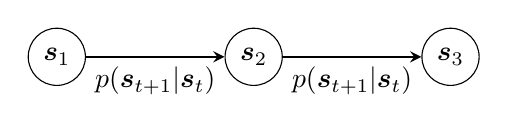
\begin{tikzpicture}[scale=1, transform shape, node distance=1.5cm]
		\node (s1) [mcs] {$\bm{s}_{1} $};
		\node (s2) [mcs, right of=s1, xshift=1cm] { $ \bm{s}_{2}  $};
		\draw [arrow] (s1) -- node [below, midway] {$ p(\bm{s}_{t+1}|\bm{s}_{t}) $} (s2);
		\node (s3) [mcs, right of=s2, xshift=1cm] { $ \bm{s}_{3}  $};
		\draw [arrow] (s2) -- node [below, midway] {$ p(\bm{s}_{t+1}|\bm{s}_{t}) $} (s3);
\end{tikzpicture}
\end{center}
\end{figure}
\begin{itemize}
\item $\mathcal{M} = \{\mathcal{S}, \mathcal{T}\}$
\item $\mathcal{S}$ - state space, $s \in \mathcal{S}$ (discrete or continuous)
\item $\mathcal{T}$ - transition operator --- for  $p(s_{t+1} | s_t)$ let 
		$\mu_{t,i} = p(s_t =i), \mathcal{T}_{i,j} = p(s_{t+1} = i  | s_t = j)$. 
		Then $\overrightarrow{\mu}_t$ is a vector of probabilities and 
		$\overrightarrow{\mu}_{t+1} = \mathcal{T} \overrightarrow{\mu}_t$
\item we have the markov property ofc
\end{itemize}
If we add actions and rewards:
\section{Markov decision process}
\begin{figure}[htpb]
\begin{center}
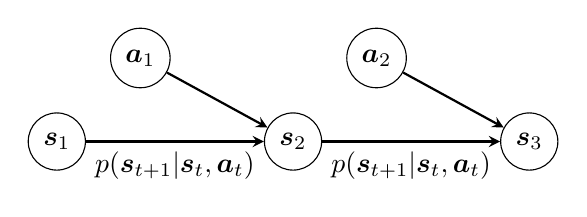
\begin{tikzpicture}[scale=1, transform shape, node distance=1.5cm]
		\node (s1) [mcs] {$\bm{s}_{1} $};
		\node (a1) [mcs, above right of=s1] { $ \bm{a}_{1}  $};
		\node (s2) [mcs, right of=s1, xshift=1.5cm] { $ \bm{s}_{2}  $};
		\draw [arrow] (a1) -- (s2);
		\draw [arrow] (s1) -- node [below, midway] {$ p(\bm{s}_{t+1}|\bm{s}_{t}, \bm{a}_{t}) $} (s2);
		\node (s3) [mcs, right of=s2, xshift=1.5cm] { $ \bm{s}_{3}  $};
		\node (a2) [mcs, above right of=s2] { $ \bm{a}_{2}  $};
		\draw [arrow] (s2) -- node [below, midway] {$ p(\bm{s}_{t+1}|\bm{s}_{t}, \bm{a}_{t}) $} (s3);
		\draw [arrow] (a2) -- (s3);
\end{tikzpicture}
\end{center}
\end{figure}
\begin{itemize}
		\item $\mathcal{M} = \{\mathcal{S}, \mathcal{A}, \mathcal{T}, r\}$
\item $\mathcal{S}$ - state space, $s \in \mathcal{S}$ (discrete or continuous)
\item $\mathcal{A}$ - action space, $a \in \mathcal{A}$ (discrete or continuous)
\item $\mathcal{T}$ - transition operator is now a tensor ---
		let $\mu_{t,j} = p(s_t = j), \xi_{t,k} = p(a_t = k), \mathcal{T}_{i,j,k} = p(s_{t+1} = i | s_t =j, a_t =k) $
		and we get $\mu_{t+1,i} = \sum_{j,k}^{} \mathcal{T}_{i,j,k} \mu_{t,j} \xi_{t,k}$
\item so the tensor version of the operator is still linear
\item $r$ - reward function ($r(s_t, a_t)$), $r : \mathcal{S} \times \mathcal{A} \to \mathbb{R}$
\end{itemize}
And if we don't have access to full states, but only partial observations of states:

\section{Partially observed Markov decision process}
\begin{figure}[htpb]
\begin{center}
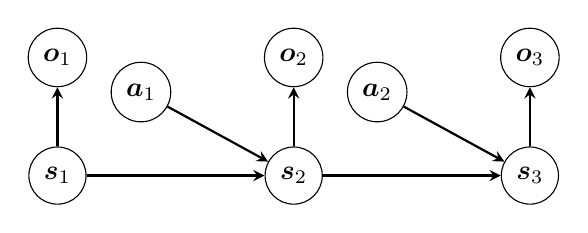
\begin{tikzpicture}[scale=1, transform shape, node distance=1.5cm]
		\node (s1) [mcs] {$\bm{s}_{1} $};
		\node (a1) [mcs, above right of=s1] { $ \bm{a}_{1}  $};
		\node (o1) [mcs, above of=s1] { $ \bm{o}_{1}  $};
		\draw [arrow] (s1) -- (o1);
		\node (s2) [mcs, right of=s1, xshift=1.5cm] { $ \bm{s}_{2}  $};
		\node (o2) [mcs, above of=s2] { $ \bm{o}_{2}  $};
		\draw [arrow] (s2) -- (o2);
		\draw [arrow] (a1) -- (s2);
		\draw [arrow] (s1) --  (s2);
		\node (s3) [mcs, right of=s2, xshift=1.5cm] { $ \bm{s}_{3}  $};
		\node (o3) [mcs, above of=s3] { $ \bm{o}_{3}  $};
		\draw [arrow] (s3) -- (o3);
		\node (a2) [mcs, above right of=s2] { $ \bm{a}_{2}  $};
		\draw [arrow] (s2) -- (s3);
		\draw [arrow] (a2) -- (s3);
\end{tikzpicture}
\end{center}
\end{figure}
\begin{itemize}
		\item $\mathcal{M} = \{\mathcal{S}, \mathcal{A}, \mathcal{O}, \mathcal{T}, \mathcal{E}, r\}$
\item $\mathcal{S}$ - state space, $s \in \mathcal{S}$ (discrete or continuous)
\item $\mathcal{A}$ - action space, $a \in \mathcal{A}$ (discrete or continuous)
\item $\mathcal{P}$ - observation space, $o \in \mathcal{O}$ (discrete or continuous)
\item $\mathcal{T}$ - transition operator (like before)
\item $\mathcal{E}$ - emission probability $p(o_t|s_t)$
\item $r$ - reward function ($r(s_t, a_t)$), $r : \mathcal{S} \times \mathcal{A} \to \mathbb{R}$
\end{itemize}

\subsection{The goal of reinforcement learning}
Let's deal with the finite horizon case for now.
\begin{equation}
\underbrace{p_\theta(\bm{s}_1, \bm{a}_1, \dots, \bm{s}_T, \bm{a}_T)}_{p_\theta(\tau)} = p(\bm{s}_1) \prod^{T}_{t=1} 
\underbrace{\pi_{\theta} (\bm{a}_t | \bm{s}_t) p (\bm{s}_{t+1} | \bm{s}_t, \bm{a}_t)}_{\text{Markov chain on} (\bm{s}, \bm{a})}
\end{equation}
A bit more explicitely:
\begin{equation}
p((\bm{s}_{t+1}, \bm{a}_{t+1}) | (\bm{s}_t, \bm{a}_t)) = 
p((\bm{s}_{t+1}| (\bm{s}_t, \bm{a}_t)) \pi_\theta (\bm{a}_{t+1} | \bm{s}_{t+1})
\end{equation}

This will allow us to define the objective a bit more conveniently.
We'll use marginalisation ( $p_\theta (\bm{s}_t, \bm{a}_t)$ is the state-action marginal) (will be useful for infinite horizon case):
\begin{align}
		\theta^\star &= \argmax_{\theta} E_{\tau \sim p_\theta(\tau)} \left[ \sum_{t}^{} r(\bm{s}_t, \bm{a}_t) \right] \\
	 &= \argmax_{\theta} \sum_{t}^{T} E_{(\bm{s}_t, \bm{a}_t) \sim p_\theta(\bm{s}_t, \bm{a}_t)} \left[  r(\bm{s}_t, \bm{a}_t) \right]
\end{align}

OK, let's do the infinite horizon case ($T = \infty $) with a stationary distribution.
One way is to do it with a discount rate $\gamma \in (0,1)$.
Does $p(\bm{s}_t, \bm{a}_t)$ convege to a stationary distribution?
It does under the ergodicity (if you can get from any state to any other state) and if the chain is aperiodic.
In symbols stationarity is $\mu = \mathcal{T}\mu$ which you get from $(\mathcal{T} - \bm{I})\mu = 0$.
Here $\mu$ is the eingenvector of $\mathcal{T}$ with eigenvalue 1 (which always exists under some regularity conditions).
\subsubsection{Note} In RL we care about \textit{expectations}.
Because of this our goals are smooth and differentiable and we get do gradient descent on them.

\section{Value functions}
Let's start with the expectation which we are trying to maximize w.r.t. $\theta$.
We'll write it out recursively (by using the chain rule of probability), obtaining nested expectations:
\begin{align}
		E_{\tau \sim p_\theta(\tau)} & \left[ \sum_{t}^{} r(\bm{s}_t, \bm{a}_t) \right] \\
		E_{\tau \sim p_\theta(\bm{s}_1)} & \left[ E_{\bm{a}_1 \sim \pi(\bm{a}_1|\bm{s}_1)}
		\left[ r(\bm{s}_1, \bm{a}_1) + E_{\bm{s}_2  \sim p(\bm{s}_2 | \bm{s}_1, \bm{a}_1)} 
\left [				E_{\bm{a}_2 \sim \pi(\bm{a}_2|\bm{s}_2)}
				\left[ r(\bm{s}_2, \bm{a}_2) + \dots | \bm{s}_2 \right] | \bm{s}_1, \bm{a}_1
\right] | \bm{s}_1  \right] \right ]
\end{align}

Enter the Q-functions:
\begin{equation}
		Q(\bm{s}_1, \bm{a}_1) = 
r(\bm{s}_1, \bm{a}_1) + E_{\bm{s}_2  \sim p(\bm{s}_2 | \bm{s}_1, \bm{a}_1)} 
\left [				E_{\bm{a}_2 \sim \pi(\bm{a}_2|\bm{s}_2)}
				\left[ r(\bm{s}_2, \bm{a}_2) + \dots | \bm{s}_2 \right] | \bm{s}_1, \bm{a}_1
\right]
\end{equation}
If we knew $Q(\bm{s}_1, \bm{a}_1)$, it would be easy to modify $\pi_\theta (\bm{s}_1, \bm{a}_1)$:
\begin{equation}
	E_{\tau \sim p_\theta(\tau)} \left[  \sum_{t=1}^{T} r(\bm{s}_t, \bm{a}_t) \right] 	
	= E_{\bm{s}_1 \sim p_\theta(\bm{s}_1)}
	\left[  E_{\bm{a}_1 \sim \pi(\bm{a}_1|\bm{s}_1)} \left[ Q(\bm{s}_1, \bm{a}_1) |\bm{s}_1 \right]   \right] 
\end{equation}
For example we could just do $\pi(\bm{s}_1, \bm{a}_1) = 1$ 
if $\bm{a}_1 = \argmax_{\bm{a}_1} Q(\bm{s}_1, \bm{a}_1)$.

\subsubsection{Definition: Q-function}
\begin{equation}
		Q^\pi (\bm{s}_t, \bm{a}_t) = \sum_{t'=t}^{T} E_{\pi_\theta}
		\left[ r(\bm{s}_{t'}, \bm{a}_{t'} )| \bm{s}_t, \bm{a}_t \right] 
\end{equation}
thus denoting the total reward from taking $\bm{a}_t$ in $\bm{s}_t$.

\subsubsection{Definition: value function}
\begin{equation}
		V^\pi (\bm{s}_t) = \sum_{t'=t}^{T} E_{\pi_\theta}
		\left[ r(\bm{s}_{t'}, \bm{a}_{t'} | \bm{s}_t) \right] 
\end{equation}
thus denoting the total (average/expected) reward from $\bm{s}_t$.

The connection between the 2 is the following:
\begin{equation}
		V^\pi (\bm{s}_t) = E_{\bm{a}_t \sim \pi(\bm{s}_t, \bm{a}_t)}
		\left[ Q^\pi(\bm{s}_t, \bm{a}_t) \right] 
\end{equation}
And we can also write the RL objective as:
\begin{equation}
		E_{\bm{s}_1 \sim p(\bm{s}_1)}
		\left[ V^\pi (\bm{s}_1) \right] 
\end{equation}

How can we use Q-functions and value functions?
One idea is the following: if we have $\pi$ and we know $Q^\pi(\bm{s}, \bm{a})$,
then we can improve $\pi$:
\begin{itemize}
		\item set $\pi'(\bm{a}|\bm{s}) = 1$ is $\bm{a} = \argmax_{\bm{a}} Q^\pi(\bm{s}, \bm{a})$
		\item this policy is at least as good as $\pi$ and is probabily better (easily provable)
		\item it does not matter what $\pi$ is, this is always true
\end{itemize}

Another idea is to compute the gradient to increase the probability of good actions $\bm{a}$:
if $ Q^\pi(\bm{s}, \bm{a}) > V^\pi(\bm{s})$ then $\bm{a}$ is \textit{better than average} (recall definition of $V^\pi(\bm{s})$ under $\pi(\bm{a}|\bm{s}) $  ).
We can then modify $\pi(\bm{a}|\bm{s})$ to increase the probabily of $\bm{a}$ if $ Q^\pi(\bm{s}, \bm{a}) > V^\pi(\bm{s})$


\chapter{Policy gradients}
\subsubsection{The idea} We are going to directly formalize the concept of trial-and-error learning.


 A trajectory distribution in MDP setting is:
 \begin{equation}
 		\underbrace{p_\theta(\bm{s}_1, \bm{a}_1, \dots, \bm{s}_T, \bm{a}_T)}_{p_\theta(\tau)} = p(\bm{s}_1) \prod^{T}_{t=1} \pi_{\theta} (\bm{a}_t | \bm{s}_t) p (\bm{s}_{t+1} | \bm{s}_t, \bm{a}_t)
 \end{equation}
The right side is the chain rule of probabilities

The objective of reinforcement learning is:
\begin{equation}
		\theta^\star = \argmax_\theta E_{\tau \sim p_\theta (\tau)} \left [ \sum_t r(\bm{s}_t, \bm{a}_t) \right ]
\end{equation}

We can push out the sum via the linearity of expectation.
This can then be expanded with a marginal for the infinite horizon.
Infinite case (can be achieved with value functions):
\begin{equation}		
		\theta^\star = \argmax_\theta E_{(\bm{s}, \bm{a}) \sim p_\theta (\bm{s}, \bm{a})} \left [r(\bm{s}, \bm{a}) \right]
\end{equation}

Finite horizon case:
\begin{equation}		
		\theta^\star = \argmax_\theta \sum^{T}_{t=1}  E_{(\bm{s}_t, \bm{a}_t) \sim p_\theta (\bm{s}_t, \bm{a}_t)} \left [ r(\bm{s}_t, \bm{a}_t) \right]
\end{equation}


Let's talk about evaluating the reinforcement learning objective.
First let's introduce a notational shorthand:

\begin{equation}
		\theta^\star = \argmax_\theta \underbrace{E_{\tau \sim p_\theta (\tau)} \left [ \sum_t r(\bm{s}_t, \bm{a}_t) \right ]}_{J(\theta)}
\end{equation}

We estimate $J(\theta)$ by making rollouts from the policy (below $i$ is the sample index and $i,t$ is the $t^{th}$ timestep
in the $i^{th}$ sample):
\begin{equation}
		J(\theta) = E_{\tau \sim p_\theta(\tau)} \left [ \sum_t r(\bm{s}_t, \bm{a}_t) \right ] \approx 
		\frac{1}{N} \sum_i \sum_t r(\bm{s}_{i,t}, \bm{a}_{i,t})
\end{equation}

Let's directly differentiate the policy.
But first some more notational shorthands:
\begin{equation}
		J(\theta) = E_{\tau \sim p_\theta(\tau)} \underbrace{[r(\tau)]}_{\sum^{T}_{t=1} r(\bm{s}_t, \bm{a}_t)} = 
		\int_{{}}^{} {p_\theta(\tau)r(\tau)} \: d{\tau} {}
\end{equation}

Now we start working on the derivative:
\begin{equation}
		\nabla_\theta J(\theta) = \int_{{}}^{{}} {\nabla_\theta p_\theta (\tau) r(\tau)} \: d{\tau} {}
\end{equation}

We'll need to use a convenient identity because we don't know $p_\theta(\tau)$ (nor its gradient):
\begin{equation}
	p_\theta(\tau) \nabla_\theta \log p_\theta(\tau) =
	p_\theta (\tau) \frac{\nabla_\theta p_\theta(\tau)}{p_\theta(\tau)} =
	\nabla_\theta p_\theta(\tau)
\end{equation}
So now:
\begin{equation}
		\nabla_\theta J(\theta) = \int_{{}}^{{}} {\nabla_\theta p_\theta (\tau) r(\tau)} \: d{\tau} {}
		=
		\int_{{}}^{{}} {p_\theta(\tau) \nabla_\theta \log  p_\theta(\tau) r(\tau) } \: d{\tau} =
		E_{\tau \sim p_\theta(\tau)} [\nabla_\theta \log p_\theta(\tau)r(\tau)]
\end{equation}
THERE ARE MISTAKES BELOW, PLEASE COME BACK AND CORRECT THEM!!!!!!!!

We can evaluate expectations with samples so we're on a good track.
We can log $p_\theta(\tau)$ on both sides of the equation and get a summation instead of a product.
Let's see what we get from that:
\begin{equation}
		\nabla_\theta \log p_\theta(\tau)r(\tau) =
\nabla_\theta \left [\cancel{\log p(\bm{s}_1)} + \sum^{T}_{t=1} \log \pi_\theta (\bm{a}_t | \bm{s}_t) + \cancel{\log p(\bm{s}_{t+1} | \bm{s}_t, \bm{a}_t)} \right ]
\end{equation}
And now what's left is:
\begin{equation}
		\nabla_\theta J(\theta) = E_{\tau \sim p_\theta(\tau)} 
		\left [ \left ( \sum_{t=1}^{T} \nabla_\theta \log \pi_\theta (\bm{a}_t | \bm{s}_t ) \right )
		\left ( \sum_{t=1}^{T} r(\bm{s}_t, \bm{a}_t) \right ) \right ]
\end{equation}

To evaluate the policy gradient we can sample:
\begin{equation}
		\nabla_\theta J(\theta) \approx \frac{1}{N}  \sum_{i=1}^{N} 
		\left ( \sum_{t=1}^{T} \nabla_\theta \log \pi_\theta (\bm{a}_{i,t} | \bm{s}_{i,t} ) \right )
		\left ( \sum_{t=1}^{T} r(\bm{s}_{i,t}, \bm{a}_{i,t}) \right )
\end{equation}
Once we have the gradient we can do a step of gradient ascent and we good to go!
This is the REINFORCE algorithm:
\begin{enumerate}
		\item sample $\{\tau^i\}$ from $\pi_\theta(\bm{a}_t | \bm{s}_t)$(run policy)
		\item $\nabla_\theta J(\theta) \approx   \sum_{i=1}^{} 
		\left ( \sum_{t=1}^{T} \nabla_\theta \log \pi_\theta (\bm{a}_{i,t} | \bm{s}_{i,t} ) \right )
		\left ( \sum_{t=1}^{T} r(\bm{s}_{i,t}, \bm{a}_{i,t}) \right )$
\item $\theta \leftarrow \theta + \alpha \nabla_\theta J(\theta) $
\end{enumerate}


If you implement this as-is, it won't work (well).
Let's discuss the algorithm a bit more.
But first, even simpler:
\begin{align}
		\nabla_\theta J(\theta) &\approx \frac{1}{N}  \sum_{i=1}^{T} 
		\left ( \sum_{t=1}^{T} \nabla_\theta \log \pi_\theta (\bm{a}_{i,t} | \bm{s}_{i,t} ) \right )
		\left ( \sum_{t=1}^{T} r(\bm{s}_{i,t}, \bm{a}_{i,t}) \right ) \\
		&\approx \frac{1}{N} \sum_{i=1}^{N} \nabla_\theta \log \pi_\theta (\tau_i)r(\tau_i)
\end{align}
Maximum likelihood:
\begin{equation}
		\nabla_\theta J_{ML}(\theta) \approx \frac{1}{N} \sum_{i=1}^{N} \nabla_\theta \log \pi_\theta (\tau_i) 
\end{equation}

In practise, we have finite samples. We also get really high variance with rewards.
Thus we need some strategy to lower the variance.

\section{Reducing variance}
\subsubsection{Causality} policy at time $t'$ cannot affect reward at time $t$ when $t<t'$.
Our algorithm thus not use this fact. Let's make it use it.
First let's rewrite the policy gradient (just used distributive property):
\begin{equation}
		\nabla_\theta J(\theta) \approx 
		\frac{1}{N} \sum_{i=1}^{N} \sum_{t=1}^{T} \nabla_\theta \log \pi_\theta (\bm{a}_{i,t}| \bm{s}_{i,t})
		\left ( \sum_{t'=1}^{T} r (\bm{s}_{i,t}, \bm{a}_{i,t}) \right )
\end{equation}

Let's change the log-probability of the action at every time step,
based on whether than action led to better actions in future, present and past.
But the past rewards will have to average out to 0 because they don't matter for future rewards.
So just sum from $t'$ to $T$ and make this unbiased:
\begin{equation}
		\label{eq:reward_to_go}
		\nabla_\theta J(\theta) \approx 
		\frac{1}{N} \sum_{i=1}^{N} \sum_{t=1}^{T} \nabla_\theta \log \pi_\theta (\bm{a}_{i,t}| \bm{s}_{i,t})
		\underbrace{\left ( \sum_{t'=t}^{T} r (\bm{s}_{i,t}, \bm{a}_{i,t}) \right )}_{\text{"reward to go"}}
\end{equation}

"Reward to go" refers to the same estimate as the Q-function!
So we can write:
\begin{equation}
		\nabla_\theta J(\theta) \approx 
		\frac{1}{N} \sum_{i=1}^{N} \sum_{t=1}^{T} \nabla_\theta \log \pi_\theta (\bm{a}_{i,t}| \bm{s}_{i,t})
		\hat{Q}_{i,t} 
\end{equation}
This will be further discussed later.

\subsection{Baselines}
If the good actions yield positive rewards and the bad actions yield negative rewards,
the policy gradient will decrease the probability of bad actions and increase the probability 
of good actions.
But what if all the rewards are positive?
Then all actions' probabilities will be increased, only by different amounts.
And that's not really what we want --- we want to increase only the probability of good actions,
and decrease the probability of bad actions.
How do we do that if the rewards are all positive?
The below is what we'd like:
\begin{align}
		\nabla_\theta J(\theta) &\approx 
		\frac{1}{N} \sum_{i=1}^{N}
		\nabla_\theta \log p_\theta (\tau) [ r(\tau) - b] \\
		b &= \frac{1}{N} \sum_{i=1}^{N} r(\tau)
\end{align}
Here $b$ is the average reward and thus we'd increase the probability of
actions which are better than average.
But are we allowed to do that?
Well, one can show that substracting a number will not change the gradient in expectation,
but it will change its variance (so the estimator will be unbiased for any b).

\begin{align}
E \left [ \nabla_\theta \log p_\theta (\tau) b \right ] &=
\int{p_\theta \nabla_\theta \log p_\theta (\tau) b}  \: d{\tau}  \\
 & =
\int{ \nabla_\theta p_\theta (\tau) b } d{\tau}  \\
 &= 
b \nabla_\theta \int { p_\theta (\tau) b } d{\tau} = b \nabla_\theta 1 = 0
\end{align}

For a finite number of samples, it won't be 0 so it will alter the variance!
Also, this is not a perfect baseline (it's good tho) . 
We will derive the perfect baseline for the knowledge gains, even though it's rarely used in practise.

\begin{align}
		\text{Var} [x] &= E[x^2] - E[x]^2 \\
		\nabla_\theta J(\theta) &= E_{\tau \sim p_\theta(\tau)} 
		\left [ \nabla_\theta \log p_\theta(\tau) (r(\tau) - b))^2 \right ]
		- E_{\tau \sim p_\theta(\tau)} 
		\underbrace{\left [ \nabla_\theta \log p_\theta(\tau) r(\tau) - b) \right ]^2}_
		{\text{is just} E_{\tau \sim p_\theta(\tau)} \left [ \nabla_\theta \log p_\theta(\tau) r(\tau) \right ]}  \\
		\frac{d \text{Var}}{db} &= \frac{d}{db} E[g(\tau)^2(r(\tau) - b)^2]
		= \frac{d}{db} (\cancel{E[g(\tau)^2r(\tau)^2]} - 2E[g(\tau)^2r(\tau)b ] + b^2 E[g(\tau)^2]) \\
								&= -2E[g(\tau)^2r(\tau)b ] + b^2 E[g(\tau)^2]) = 0\\
b &= \frac{E[g(\tau)^2r(\tau)b ]}{E[g(\tau)^2])} 
\end{align}
So this is the optimal $b$ (the baseline which minimizes the variance).
You'll have a different baseline for every parameter as
this is just the expected reward, by weigthed by gradient magnitudes.

\section{Off-policy gradients}
Let's first discuss why policy gradients are an on-policy method (the classic one in fact).
\begin{equation}
		\nabla_\theta J(\theta) = \underbrace{E_{\tau \sim p_\theta(\tau)}}_{\text{this is the trouble!}} [\nabla_\theta p_\theta(\tau)r(\tau)]
\end{equation}
We need samples according to $\theta$ and hence we can't retain data from other policies, or even 
the previous versions of our own policy (we can't skip step 1 in the REINFORCE algorithm).
Neural networks require small gradients ('cos they are nonlinear).
So if generating samples is expensive, this will be bad (on the other hand,
if they're not, this will be nice).

What if we don't have samples from $p_\theta(\tau)$, but we have let's say
$\bar{p}(\tau)$.
Well, we can use importance sampling.
\subsubsection{Importance sampling}
\begin{align}
		E_{x \sim p(x)} [f(x)]  
		&= \int_{{}}^{{}} {p(x)f(x)} \: d{x} \\
		&= \int_{{}}^{{}} {\frac{q(x)}{q(x)}  p(x)f(x)} \: d{x} \\
		&= \int_{{}}^{{}} { q(x) \frac{p(x)}{q(x)}  f(x)} \: d{x} \\
		&= E_{x \sim p(x)} \left [ \frac{p(x)}{q(x)} f(x) \right ]
\end{align}
This is all exact (in expectation).

The importance-sampled version of the RL objective is then:
\begin{equation}
		J(\theta) = E_{\tau \sim \bar{p}(\tau)} \left [ \frac{p_\theta(\tau)}{\bar{p}(\tau)} r(\tau) \right ]
\end{equation}
Let's write out the trajectory probability distribution and see what we get:
\begin{align}
		p_\theta(\tau) &= p(\bm{s}_1) \prod_{t=1}^{T} \pi_\theta(\bm{a}_t | \bm{s}_t) p(\bm{s}_{t+1}|\bm{s}_t, \bm{a}_t) \\
		\frac{p_\theta(\tau)}{\bar{p}(\tau)} &=
		\frac{\cancel{p(\bm{s}_1)} \prod_{t=1}^{T} \pi_\theta(\bm{a}_t | \bm{s}_t) \cancel{p(\bm{s}_{t+1}|\bm{s}_t, \bm{a}_t)} }
		{\cancel{p(\bm{s}_1)} \prod_{t=1}^{T} \bar{\pi}_\theta(\bm{a}_t | \bm{s}_t) \cancel{p(\bm{s}_{t+1}|\bm{s}_t, \bm{a}_t)} } \\
	&= \frac{ \prod_{t=1}^{T} \pi_\theta(\bm{a}_t | \bm{s}_t)  }
		{ \prod_{t=1}^{T} \bar{\pi}_\theta(\bm{a}_t | \bm{s}_t)  }
\end{align}

Now we will derive the policy gradient with importance sampling.
Let's do a quick recap of where we're at:
\begin{align}
		\theta^\star  &= \argmax_\theta J(\theta) \\
		J(\theta) &= E_{\tau \sim p_\theta(\tau)} \left[ r(\tau) \right] 
\end{align}

and we want:
\begin{align}
		J(\theta') &= E_{\tau \sim p_\theta(\tau)} \left[ \frac{p_{\theta'}(\tau)}{p_\theta} r(\tau)  \right] \\
		\nabla_{\theta'}	J(\theta') &= E_{\tau \sim p_\theta(\tau)} \left[ \frac{\nabla_{\theta'} p_{\theta'}(\tau)}{p_\theta} r(\tau)  \right] \\
	   &= E_{\tau \sim p_\theta(\tau)} \left[  \frac{p_{\theta'}(\tau)}{p_\theta(\tau)} \nabla_{\theta'} \log p_{\theta'}(\tau)r(\tau) \right] 
\end{align}
If you estimate locally, at $\theta = \theta'$: 
\begin{equation}
\nabla_\theta J(\theta)  = E_{\tau \sim p_\theta(\tau)} \left[ \nabla_\theta \log p_\theta(\tau)r(\tau) \right] 
\end{equation}
thus getting the same gradient.
But if they're not the same:

\begin{align}
		\nabla_{\theta} J(\theta') &= E_{\tau \sim p_\theta(\tau)} \left[ \frac{p_{\theta'}(\tau)}{p_\theta} 
				\nabla_{\theta'} (\tau)
		r(\tau)  \right] \text{  when } \theta \neq \theta' \\
	=& E_{\tau \sim p_\theta(\tau)}
	\left[ 
			\left( \prod_{t=1}^{T} \frac{\pi_{\theta'} (\bm{a}_t | \bm{s}_t)}{\pi_\theta(\bm{a}_t | \bm{s}_t)}   \right) 
			\left( \sum_{t=1}^{T} \nabla_{\theta'} \log \pi_{\theta'}(\bm{a}_t | \bm{s}_t) \right) 
			\left( \sum_{t=1}^{T} r(\bm{s}_t, \bm{a}_t) \right) 
	\right] \\
	=& E_{\tau \sim p_\theta(\tau)}
	\left[ 
			\sum_{t=1}^{T} \nabla_{\theta'} \log \pi_{\theta'}(\bm{a}_t | \bm{s}_t)
			\left( \prod_{t'=1}^{t} \frac{\pi_{\theta'} (\bm{a}_{t'} | \bm{s}_{t'})}{\pi_\theta(\bm{a}_{t'} | \bm{s}_{t'})}   \right) 
			\left( \sum_{t=1}^{T} r(\bm{s}_{t'}, \bm{a}_{t'}) 
					\left( \prod_{t''=t}^{t'} \frac{\pi_{\theta'}(\bm{a}_{t''}|\bm{s}_{t''})}{\pi_{\theta}(\bm{a}_{t''}|\bm{s}_{t''})}  \right) 
			\right) 
	\right] 
\end{align}
where for the last equality we used the fact that future actions don't affect the current weight.

If we ignore $\prod_{t''=t}^{t'} \frac{\pi_{\theta'}(\bm{a}_{t''}|\bm{s}_{t''})}{\pi_{\theta}(\bm{a}_{t''}|\bm{s}_{t''})} $,
we get a policy iteration algorithm (will be covered later).
Then we won't have gradient, but we'll still improve our policy.

The problem lies in $\prod_{t'=1}^{t} \frac{\pi_{\theta'} (\bm{a}_{t'} | \bm{s}_{t'})}{\pi_\theta(\bm{a}_{t'} | \bm{s}_{t'})}$.
The reason is that it is exponential in $T$.
Let's say that the importance weights are all less than 1 (totally plausible).
Then their product will go to 0 exponentially fast and that's bad for numerical reasons.
So let's write the objective a bit differently.
The on-policy policy gradient is:
\begin{equation}
		\nabla_\theta J(\theta) \approx
		\frac{1}{N} \sum_{i=1}^{N} \sum_{t=1}^{T} \nabla_\theta \log \pi_\theta(\bm{a}_{i,t}|\bm{s}_{i,t} \hat{Q}_{i,t} )
\end{equation}
where $(\bm{s}_{t,i}, \bm{a}_{t,i}) \sim \pi_\theta(\bm{s}_{t,i}, \bm{a}_{t,i})$
The a different Off-policy policy gradient would be:
\begin{equation}
		\nabla_{\theta'} J(\theta') \approx
		\frac{1}{N} \sum_{i=1}^{N} \sum_{t=1}^{T} 
		\frac{\pi_{\theta'}(\bm{s}_{i,t}, \bm{a}_{i,t})}{\pi_{\theta}(\bm{s}_{i,t}, \bm{a}_{i,t})} 
		\nabla_{\theta'} \log \pi_{\theta'} (\bm{s}_{i,t}, \bm{a}_{i,t}) 
		\hat{Q}_{i,t} 
\end{equation}
Not useful 'cos you can't calculate probabilities of the marginals.
But we can split it via chain rule and ignore the state marginals:
\begin{equation}
		\nabla_{\theta'} J(\theta') \approx
		\frac{1}{N} \sum_{i=1}^{N} \sum_{t=1}^{T}
		\cancel{\frac{\pi_{\theta'}(\bm{s}_{i,t})}{\pi_{\theta}(\bm{s}_{i,t})}  }
		\frac{\pi_{\theta'}( \bm{a}_{i,t} | \bm{s}_{i,t})}{\pi_{\theta}( \bm{a}_{i,t} | \bm{s}_{i,t})} 
		\nabla_{\theta'} \log \pi_{\theta'} (\bm{s}_{i,t}, \bm{a}_{i,t}) 
		\hat{Q}_{i,t} 
\end{equation}
This does not in general give the correct policy gradient, but its reasonable
in the sense that it gives bounded error is $\pi_{\theta'}$ is no too different form $\pi_\theta$.
But that will be discussed later.

\subsection{Policy gradient with automatic differentiation}
We don't want to calculate the grad for every state-action pair 'cos neural nets have a lot of 
parameters.
Typically we want to use the backpropagation algorithm.
Thus we need to set our computational graph so that its gradient is the policy gradient.
So we'll implement a ``pseudo-loss'' as a weighet maximum likelihood:
\begin{equation}
		\tilde{J}(\theta) \approx \frac{1}{N} \sum_{i=1}^{N} \sum_{t=1}^{T} \log \pi_\theta(\bm{a}_{i,t} | \bm{s}_{i,t}) \hat{Q}_{i,t}
\end{equation}
This equation means nothing, but it will give us the gradient that we want (lol).

\subsection{Policy gradients in practice}
\begin{itemize}
		\item gradient has high variance, so use very large batch sizes (in the thousands)
		\item tweaking learning rates is very hard (ADAM can be OK-ish), we'll do specific stuff on this later.
\end{itemize}

\section{Advanced policy gradients}
(There will be more on this later (even more advanced policy gradients (lol)).
We have the following problem: some parameters change probabilities a lot more than others!
We'd like to increase the changes made by parameters that make small changes, and decrease
the effect of the parameters which make the larger changes.
To see why this is necessary, imagine a vector field which does not point directly to the goal because
a certain direction is too dominant.
This problem is also similar to that of poor-performing gradient descent --- the one which goes zig-zag instead of going
straight to the goal. In short, we're dealing with a common problem in optimization.

The idea is to rescale the gradient so that that doesn't happen.
So instead of doing
\begin{equation}
		\theta' \leftarrow \argmax_{\theta'} (\theta' - \theta)^T \nabla_{\theta}J(\theta) \text{ s.t. } ||\theta' - \theta||^2 \leq \epsilon
\end{equation}
we can do
\begin{equation}
		\theta' \leftarrow \argmax_{\theta'} (\theta' - \theta)^T \nabla_{\theta}J(\theta) \text{ s.t. } D(\pi_{\theta'}, \pi_\theta) \leq \epsilon
\end{equation}
where $D(\pi_{\theta'}, \pi_\theta)$ is the parametrization-independent divergence measure.
usually the KL-divergence:
\begin{equation}
		D_{KL} (\pi_{\theta'}||\pi_\theta) = E_{\pi_{\theta'}} \left[ \log \pi_\theta - \log \pi_{\theta'} \right]  
		\approx (\theta' - \theta)^T \bm{F} (\theta' - \theta)
\end{equation}
where $\bm{F}$ is the Fisher-information matrix which can be estimated with samples:
\begin{equation}
		\bm{F} = E_{\pi_{\theta}} \left[ \nabla_{\theta} \log \pi_\theta(\bm{a}|\bm{s}) \nabla_{\theta} \log \pi_\theta(\bm{a}|\bm{s})^T \right] 
\end{equation}

So for the natural gradient pick $\alpha$.
For trust region policy optimization pick $\epsilon$.
Then solve for optimal $\alpha$ while solving $\bm{F}^{-1} \nabla_\theta J(\theta)$.
Here conjugate gradient works well.


\chapter{Actor-critic algorithms}

\begin{equation}
		\nabla_\theta J(\theta) \approx 
		\frac{1}{N} \sum_{i=1}^{N} \sum_{t=1}^{T} \nabla_\theta \log \pi_\theta (\bm{a}_{i,t}| \bm{s}_{i,t})
		\underbrace{\underbrace{\left ( \sum_{t'=t}^{T} r (\bm{s}_{i,t}, \bm{a}_{i,t}) \right )}_{\text{"reward to go"}}}_{\hat{Q}_{i,t}}
\end{equation}

$\hat{Q}_{i,t}$ estimates the expected reward if we take $\bm{a}_{i,t}$ in state $\bm{s}_{i,t}$.
Can we get a better estimate? This is just a single-run Monte-Carlo estimate.
Could we get the full expectation?
In math, can we replace $\hat{Q}_{i,t} \approx  \sum_{t'=t}^{T} r (\bm{s}_{i,t}, \bm{a}_{i,t}) $ with 
$\hat{Q}_{i,t} \approx  \sum_{t'=t}^{T} E_{\pi_\theta} \left[ r(\bm{s}_{t'}, \bm{a}_{t'}) |\bm{s}_{t}, \bm{a}_{t}  \right]   $?

Having the correct full expectation (the correct Q-function), we'd have much lower variance policy gradient.
We can also apply a baseline to this:
\begin{align}
		Q(\bm{s}_{t}, \bm{a}_{t}) &= \sum_{t'=t}^{T} E_{\pi_\theta} \left[ r(\bm{s}_{t'}, \bm{a}_{t'}) |\bm{s}_{t}, \bm{a}_{t}  \right] \text{ true \textit{expected} reward-to-go} \\
		\nabla_\theta J(\theta) &\approx \frac{1}{N} \sum_{i=1}^{N} \sum_{t=1}^{T} \nabla_\theta \log \pi_\theta (\bm{a}_{i,t}| \bm{s}_{i,t})
( Q(\bm{s}_{i,t}, \bm{a}_{i,t}) - b) \\
		b_t &= \frac{1}{N} \sum_{i}^{} Q(\bm{s}_{i,t}, \bm{a}_{i,t})
\end{align}
If we make the baseline depend on the action, that will lead to bias.
But it can depend on the state.
So we can use
\begin{equation}
		V(\bm{s}_t) = E_{\bm{a}_t \sim \pi_\theta (\bm{s}_{t}, \bm{a}_{t})} [Q(\bm{s}_{t}, \bm{a}_{t})]
\end{equation}
Then we can substract the value function from the Q-value and we get an estimate of how much
an action is better than the average.
This difference is so important that we call it the \textbf{advantage function}.
So,
\begin{align}
Q^\pi (\bm{s}_{t}, \bm{a}_{t}) & = \sum_{t'=t}^{T} E_{\pi_\theta} \left[ r(\bm{s}_{t'}, \bm{a}_{t'})|\bm{s}_t, \bm{a}_t \right] \text{ total reward from } \bm{a}_t \text{ in } \bm{s}_t\\
V^\pi (\bm{s}_t) &= E_{\bm{a}_t \sim \pi_\theta(\bm{a}_t|\bm{s}_t)} \left[ Q^\pi (\bm{s}_{t}, \bm{a}_{t}) \right]  \text{ total reward from } \bm{s}_t\\
A^\pi (\bm{s}_{t}, \bm{a}_{t}) &= Q^\pi (\bm{s}_{t}, \bm{a}_{t}) - V^\pi (\bm{s}_t)\text{ how much better } \bm{a}_t \text{ is } \\
\nabla_\theta J(\theta) & \approx \frac{1}{N} \sum_{i=1}^{N} \sum_{t=1}^{T} \nabla_{\theta} \log \pi_\theta(\bm{s}_{i,t}, \bm{a}_{i,t}) A^\pi(\bm{s}_{i,t}, \bm{a}_{i,t})
\end{align}
The better the estimate of the advantage, the lower the variance will be.
However, since it is only approximate, it will introduce a bias. But we're OK with this tradeoff.
To repeat, the below is the unbiased, but high variance single-sample estimate.

\begin{equation}
\nabla_\theta J(\theta)  \approx \frac{1}{N} \sum_{i=1}^{N} \sum_{t=1}^{T} \nabla_{\theta} \log \pi_\theta(\bm{s}_{i,t}, \bm{a}_{i,t}) 
\left( \sum_{t'=1}^{T} r(\bm{s}_{i,t'}, \bm{a}_{i,t'}) -b \right) 
\end{equation}

But should we fit $Q^\pi, V^\pi$ or $A^\pi$?
One option:
\begin{align}
Q^\pi (\bm{s}_{t}, \bm{a}_{t})  &= r(\bm{s}_{t'}, \bm{a}_{t'}) + \underbrace{\sum_{t'=t+1}^{T} E_{\pi_\theta} \left[ r(\bm{s}_{t'}, \bm{a}_{t'})|\bm{s}_t, \bm{a}_t \right]}_{V^\pi(\bm{s}_{t+1})} \\
Q^\pi (\bm{s}_{t}, \bm{a}_{t})  &= r(\bm{s}_{t}, \bm{a}_{t}) + E_{\bm{s}_{t+1} \sim p(\bm{s}_{t+1}|\bm{s}_t, \bm{a}_t)} \left[ V^\pi (\bm{s}_{t+1}) \right] 
\end{align}

Another option:
\begin{align}
		Q^{\pi} (\bm{s}_{t}, \bm{a}_{t})  &\approx r(\bm{s}_{t}, \bm{a}_{t}) + V^\pi (\bm{s}_{t+1}) \\
		A^\pi (\bm{s}_{t}, \bm{a}_{t})  &\approx r(\bm{s}_{t}, \bm{a}_{t}) + V^\pi (\bm{s}_{t+1})  - V^\pi(\bm{s}_t)
\end{align}
We like the second option because we need to learn $V^\pi(\bm{s})$ because it depends only on the state.
Since there are less states than state-actions, it should be easier to learn.
There are methods which go for option 1, but we'll dicuss those later.

OK, how do we learn $V^\pi(\bm{s})$ (it will be a neural net ofc).
We need to evaluate the policy.

\section{Policy evaluation}
\begin{align}
		V^\pi(\bm{s}_t) &= \sum_{t'=t}^{T} E_{\pi_\theta} \left[ r(\bm{s}_{t}, \bm{a}_{t})\bm{s}_t \right] \\
		J(\theta) &= E_{\bm{s}_1 \sim p(\bm{s}_1} \left[ V^\pi (\bm{s}_1) \right] 
\end{align}

How can we perform policy evaluation? 
Use Monte Carlo policy evaluation (this is what policy gradient does), i.e.
\begin{align}
		V^\pi (\bm{s}_t) &\approx \sum_{t'=t}^{T} r(\bm{s}_{t'}, \bm{a}_{t'})\\
V^\pi (\bm{s}_t) &\approx \frac{1}{N} \sum_{i=1}^{N} \sum_{t'=t}^{T} r(\bm{s}_{t'}, \bm{a}_{t'})
\end{align}
Unfortunatelly, we can't do the second thing in general (as you'd need to reset the simulator and obtain 
another trajectory from that state (and in general we can only reset to the inital state)).
Fortunatelly, if we use a neural network to fit the value function, the network will generalize between similar states ---
similar states will have similar values. This is especially cool when we're working in continuous settings.
So $V^\pi (\bm{s}_t) \approx \sum_{t'=t}^{T} r(\bm{s}_{t'}, \bm{a}_{t'})$ will still be pretty good.

Thus we do the following: we run the policy and get the training data:
\begin{equation}
		\left\{ \left( \bm{s}_{i,t}, \underbrace{\sum_{t'=t}^{T} r(\bm{s}_{i,t}, \bm{a}_{i,t})}_{y_{i,t}} \right)  \right\} 
\end{equation}
We then do supervised regresion:
\begin{equation}
		\mathcal{L}(\phi) = \frac{1}{2} \sum_{i}^{} ||\hat{V}^\pi_\phi (\bm{s}_i) - y_i||^2
\end{equation}

But can we do even better (here we substitute the reward-to-go from the $\bm{s}_{t+1}$ with the appropriate value function):
\begin{equation}
		\text{ideal target } y_{i,t} = \sum_{t'=t}^{T} E_{\pi_\theta} \left[ r(\bm{s}_{t'}, \bm{a}_{t'})|\bm{s}_{i,t}\right] + V^\pi(\bm{s}_{i,t+1})  
		\approx r(\bm{s}_{i,t}, \bm{a}_{i,t}) + \hat{V}^\pi_\phi(\bm{s}_{i,t+1}) 
\end{equation}

Thus we get a bootstrapped estimate.
Our training data becomes:
\begin{equation}
		\left\{ \left( \bm{s}_{i,t}, \underbrace{r(\bm{s}_{i,t}, \bm{a}_{i,t}) + \hat{V}^\pi_\phi(\bm{s}_{i,t+1}) }_{y_{i,t}} \right)  \right\} 
\end{equation}
We then again do supervised regresion:
\begin{equation}
		\mathcal{L}(\phi) = \frac{1}{2} \sum_{i}^{} ||\hat{V}^\pi_\phi (\bm{s}_i) - y_i||^2
\end{equation}
So again we have lower variance and higher bias (because $\hat{V}^\pi_\phi$ can (will) be incorrect).

The value functions are very intuitive. For example, in board games,
it tells you how likely you are to win in a given board state.
Also, in this particular example it is very easy to restart from a given board state 
and get better estimates for the value function in that state.

\section{From evaluation to actor-critic}
Basic example actor-critic algorithm:
\begin{enumerate}
		\item sample $\left\{ \bm{s}_i, \bm{a}_i \right\}$  from  $\pi_\theta (\bm{a}|\bm{s})$ (run policy)
		\item fit $ \hat{V}^\pi_\theta(\bm{s})$ to sampled reward sums
		\item evaluate $\hat{A}^\pi (\bm{s}_{i}, \bm{a}_{i}) = r(\bm{s}_{i}, \bm{a}_{i}) + \hat{V}^\pi_\theta(\bm{s}_i') - \hat{V}^\pi_\theta(\bm{s}_i) $
		\item $\nabla_\theta J(\theta) \approx \sum_{i}^{} \nabla_{\theta} \log \pi_\theta (\bm{a}_i|\bm{s}_i) \hat{A}^\pi (\bm{s}_{i}, \bm{a}_{i})$
		\item $\theta \leftarrow \theta + \alpha \nabla_\theta J(\theta)$
\end{enumerate}

\section{Aside: discount factors}
In infinite-episode length the value-function can get infinitely large.
So we'll discount the reward from states with $\gamma, \gamma \in [0,1]$,
\begin{equation}
		y_{i,t} \approx r(\bm{s}_{i,t}, \bm{a}_{i,t}) + \gamma \hat{V}^\pi_\theta(\bm{s}_{i, t+1})
\end{equation}
Can we do the same for (Monte Carlo) policy gradients?:
\begin{align}
\text{option 1: } & \nabla_\theta J(\theta) \approx \frac{1}{N} \sum_{i=1}^{N} \sum_{t=1}^{T} \nabla_{\theta} \log \pi_\theta(\bm{s}_{i,t}, \bm{a}_{i,t})
\left( \sum_{t'=t}^{T} \gamma^{t'-t} r(\bm{s}_{i,t'}, \bm{a}_{i,t'}) \right) \\ 
\text{option 2: } & \nabla_\theta J(\theta) \approx \frac{1}{N} \sum_{i=1}^{N}  \left( \sum_{t=1}^{T} \nabla_{\theta} \log \pi_\theta(\bm{s}_{i,t}, \bm{a}_{i,t}) \right)
\left( \sum_{t=1}^{T} \gamma^{t-1} r(\bm{s}_{i,t'}, \bm{a}_{i,t'}) \right) \\
				  &
\nabla_\theta J(\theta) \approx \frac{1}{N} \sum_{i=1}^{N}   \sum_{t=1}^{T} \nabla_{\theta} \log \pi_\theta(\bm{s}_{i,t}, \bm{a}_{i,t}) 
\left( \sum_{t'=t}^{T} \gamma^{t-1} r(\bm{s}_{i,t'}, \bm{a}_{i,t'}) \right)\\
				  &
				  \nabla_\theta J(\theta) \approx \frac{1}{N} \sum_{i=1}^{N}   \sum_{t=1}^{T} \gamma^{t-1} \nabla_{\theta} \log \pi_\theta(\bm{s}_{i,t}, \bm{a}_{i,t}) 
\left( \sum_{t'=t}^{T} \gamma^{t'-t} r(\bm{s}_{i,t'}, \bm{a}_{i,t'}) \right)
\end{align}
So the second option also discounts the importance of a decision in later steps (i.e. it discounts future gradients as well),
which makes it more correct if we want to do discounts.
But do we want the later steps to matter less?
In practise we use option 1 more often  because we don't really want the discounted problem,
we just want to use the discount to get finite values for our value functions.
That also makes our variance smaller.
We actually want the average reward, but that's impractical and that's why we use the discount factor.

%if we had a critic we'd get:
%\begin{equation}
%		\nabla_\theta J(\theta) \approx \frac{1}{N} \sum_{i=1}^{N} \sum_{t=1}^{T} \nabla_{\theta} \log \pi_\theta(\bm{s}_{i,t}, \bm{a}_{i,t})
%		\left( r(\bm{s}_{i,t}, \bm{a}_{i,t}) + \gamma \hat{V}^\pi_\theta(\bm{s}_{i,t+1}) - \hat{V}^\pi_\theta(\bm{s}_{i,t}) \right) 
%\end{equation}

Let's now create an online actor-critic algorithm:
\begin{enumerate}
		\item take action $\bm{a} \sim \pi_\theta(\bm{a}|\bm{s})$, get $(\bm{s}, \bm{a},\bm{s'},r)$
		\item update $\hat{V}^\pi_\theta$ using target $r + \gamma \hat{V}^\pi_\theta(\bm{s'})$
		\item evaluate $\hat{A}^\pi(\bm{s}_{}, \bm{a}_{})  = r(\bm{s}_{}, \bm{a}_{}) + \gamma \hat{V}^\pi_\theta(\bm{s'}) - \hat{V}^\pi_\theta(\bm{s})$
		\item $\nabla_\theta J(\theta) \approx \nabla_{\theta} \log \pi_\theta(\bm{a}|\bm{s})\hat{A}^\pi(\bm{s}_{}, \bm{a}_{})$
		\item $\theta \leftarrow \theta  + \alpha \nabla_\theta J(\theta)$
\end{enumerate}

\section{Actor-critic design choises}

We can do a two network design: one for the value function $\bm{s} \to \hat{V}^\pi_\theta(\bm{s})$ and one for the policy 
$\bm{s} \to \pi_\theta(\bm{a}|\bm{s})$.
The good thing about this is simple and stable. The bad thing is that it has no shared features between the actor and the critic.
Alternatively, you can go for the shared network desing (have a single network for both).
It will probably need more hyperparameter tuning, but it is in principle more efficient.

\section{Online actor-critic in practise}
In practice (due to the properties of neural networks) we want to update with batches and not do a single sample gradient.
One way to get a batch is to use multiple works, i.e. do the synchronized parallel actor-critic.
This way you'll get n\_workers-sized batches.
The alternative is to do the asynchronous parallel actor-critic.
In general you'll get samples from different actors with approach (there is some lag in different threads).
This makes it mathematically incorrect, but in practise this leads to overall performance benefits (because the actors are not that different,
because the lag is not so large (all workers are running the same program after all (if they don't hang up that is lol))).

Cool. But it could be even better to use an off-policy actor-critic.
However, to do so we need to modify the algorithm.
We'd do this:
\begin{enumerate}
		\item take action $\bm{a} \sim \pi_\theta(\bm{a}|\bm{s})$, get $(\bm{s}, \bm{a},\bm{s'},r)$, store in $\mathcal{R}$ (replay buffer)
		\item sample a batch $\left\{  (\bm{s}_i, \bm{a}_i,\bm{s'}_i,r_i) \right\} $ from buffer $\mathcal{R}$
		\item update $\hat{V}^\pi_\theta$ using target $y_i = r_i + \gamma \hat{V}^\pi_\theta(\bm{s'}_i)$
		\item evaluate $\hat{A}^\pi(\bm{s}_{i}, \bm{a}_{i})  = r(\bm{s}_{i}, \bm{a}_{i}) + \gamma \hat{V}^\pi_\theta(\bm{s}_i') - \hat{V}^\pi_\theta(\bm{s}_i)$
		\item $\nabla_\theta J(\theta) \approx  \frac{1}{N} \sum_{i}^{}  \nabla_{\theta} \log \pi_\theta(\bm{a}_i|\bm{s}_i)\hat{A}^\pi(\bm{s}_{i}, \bm{a}_{i})$
		\item $\theta \leftarrow \theta  + \alpha \nabla_\theta J(\theta)$
\end{enumerate}
where  $\mathcal{L}(\phi) = \frac{1}{N} \sum_{i}^{} || \hat{V}^\pi_\theta(\bm{s}_i) - y_i||^2 $.

Unfortunatelly, this algorithm is broken!
Firstly, $y_i = r_i + \gamma \hat{V}^\pi_\theta(\bm{s'}_i)$ will not give you the target value 
of the current actor, but a past actor: $\bm{a}_i$ did not come from $\pi_\theta$
and therefore $\bm{s}_i'$ didn't either.
Likewise, the policy gradient $\nabla_{\theta} \log \pi_\theta(\bm{a}_i|\bm{s}_i)$ is also wrong for the same reason.
To solve this, we could use importance sampling (or something else (soon...)).
Let's first fix the value function.
Well, the value function tells us the expected reward if we start in state $\bm{s}_t$ and the follow the policy $\pi$ onward,
the Q-function tells you the expected reward if you start in state $\bm{s}_t$ and take action $\bm{a}_t$ and then 
follow the policy $\pi$.
Notice that in the Q-function it doesn't matter if $\bm{a}_t$ was taken from policy $\pi$.
Thus it is valid for any action, it's just that in all subsequent steps $\pi$ needs to be followed.
So to solve the problem, we'll learn $Q^\pi(\bm{s}_{t}, \bm{a}_{t})$ instead of $V^\pi(\bm{s}_t)$.
We do this by updating $\hat{Q}^\pi_\phi $ using the targets
$y_i = r_i + \gamma \hat{V}^\pi_\theta(\bm{s}') \forall \bm{s}_i, \bm{a}_i$.
We still need $\hat{V}$ for the target values however.
But we can use:
\begin{equation}
		V^\pi(\bm{s}_t) = \sum_{t'=t}^{T} E_{\pi\theta} \left[ r(\bm{s}_{t'}, \bm{a}_{t'})|\bm{s}_t \right] = E_{\bm{a} \sim \pi(\bm{a}_t | \bm{s}_t)} \left[ Q(\bm{s}_{t}, \bm{a}_{t}) \right] 
\end{equation}

Now we can update $\hat{Q}^\pi_\phi$ using
\begin{align}
		y_i &= r_i + \gamma \hat{V}^\pi_\theta(\bm{s}')\forall \bm{s}_i, \bm{a}_i \\
			&= r_i + \gamma \hat{Q}^\pi_\phi(\bm{s}_{i}', \underbrace{\underbrace{\bm{a}_{i}'}_{  \text{not from replay buffer }\mathcal{R}}}_{\bm{a}_i' \sim \pi_\theta(\bm{a}_i'|\bm{s}_i')})
\end{align}
This works because you don't need to interact with the simulator to ask which action your current network would have taken 
if it found itself in this (old) state (even though it never got there itself).

Now we'll deal with the policy gradient and we'll do the same trick, but for $\bm{a}_i$ instead of $\bm{a}_i'$
Thus we'll sample $\bm{a}_i^\pi \sim \pi_\theta(\bm{a}|\bm{s}_i)$ and get the following gradient:
\begin{equation}
		\nabla_\theta J(\theta) \approx \frac{1}{N} \sum_{i}^{} \nabla_{\theta}\log \pi_\theta(\bm{a}_i^\pi|\bm{s}_i) \hat{A}^\pi (\bm{s}_{i}, \bm{a}_{i}^\pi)
\end{equation}
where $\bm{a}_i^\pi$ is not from the replay buffer $\mathcal{B}$.
But in practice we don't actually use advantages:
\begin{equation}
		\nabla_\theta J(\theta) \approx \frac{1}{N} \sum_{i}^{} \nabla_{\theta}\log \pi_\theta(\bm{a}_i^\pi|\bm{s}_i) \hat{Q}^\pi (\bm{s}_{i}, \bm{a}_{i}^\pi)
\end{equation}
This will lead to higher variance, but we don't really care because we don't need to interact the simulator
and we can thus lower the variance by generating more samples (just run the network a few more times, no need for more state).

There are still problems with the current version of our off-policy actor-critic algorithm.
Namely, $\bm{s}_i$ didn't come from $p_\theta(\bm{s})$. Unfortunatelly, we
can't do anything about this.
Fortunatelly, we'll get an optimal policy on a broader distribution. Yes, it will be more work 
due to the higher variance, but the final result will be better.
So in total we're left with:
\begin{enumerate}
		\item take action $\bm{a} \sim \pi_\theta(\bm{a}|\bm{s})$, get $(\bm{s}, \bm{a},\bm{s'},r)$, store in $\mathcal{R}$ (replay buffer)
		\item sample a batch $\left\{  (\bm{s}_i, \bm{a}_i,\bm{s'}_i,r_i) \right\} $ from buffer $\mathcal{R}$
		\item update $\hat{Q}^\pi_\theta$ using target $y_i = r_i + \gamma \hat{Q}^\pi_\theta(\bm{s}_i', \bm{a}_i') \forall \bm{s}_i, \bm{a}_i$
		\item $\nabla_\theta J(\theta) \approx  \frac{1}{N} \sum_{i}^{}  \nabla_{\theta} \log \pi_\theta(\bm{a}^\pi_i|\bm{s}_i)\hat{Q}^\pi(\bm{s}_{i}, \bm{a}^\pi_{i})$,
				where $\bm{a}_i^\pi \sim \pi_\theta(\bm{a} | \bm{s}_i)$
		\item $\theta \leftarrow \theta  + \alpha \nabla_\theta J(\theta)$
\end{enumerate}
In practise, people use the reparametrization trick in the gradient estimate and get a better estimate with it.
Furthermore, there are a lot of fancier ways to fit Q-functions (for example soft actor-critic (SAC)).

\section{Critics as state-dependent baselines}
Let's first restate the actor-critic policy gradient:
\begin{equation}
	\nabla_\theta J(\theta) \approx \frac{1}{N} \sum_{i=1}^{N} \sum_{t=1}^{T} \nabla_{\theta} \log \pi_\theta(\bm{s}_{i,t}, \bm{a}_{i,t})
		\left( r(\bm{s}_{i,t}, \bm{a}_{i,t}) + \gamma \hat{V}^\pi_\theta(\bm{s}_{i,t+1}) - \hat{V}^\pi_\theta(\bm{s}_{i,t}) \right) 
\end{equation}
and the policy gradient:
\begin{equation}
		\nabla_\theta J(\theta) \approx \frac{1}{N} \sum_{i=1}^{N} \sum_{t=1}^{T} \nabla_{\theta} \log \pi_\theta(\bm{s}_{i,t}, \bm{a}_{i,t})
		\left( \left( \sum_{t'=t}^{T} \gamma^{t' -t} r(\bm{s}_{i,t'}, \bm{a}_{i,t'}) \right) -b \right) 
\end{equation}
More recap: the actor-critic policy gradient has much lower variance (due to the critic), but it is biased (if the critic is not perfect).
On the other hand, the policy gradient has no bias, but it has high variance (because it uses a single-sample estimate).
Now a question: can we have an ubiased policy gradient and still use the critic to reduce the variance?
The way to do this is to use a state-dependent baseline, namely:
\begin{equation}
		\nabla_\theta J(\theta) \approx \frac{1}{N} \sum_{i=1}^{N} \sum_{t=1}^{T} \nabla_{\theta} \log \pi_\theta(\bm{s}_{i,t}, \bm{a}_{i,t})
		\left( \left( \sum_{t'=t}^{T} \gamma^{t' -t} r(\bm{s}_{i,t'}, \bm{a}_{i,t'}) \right)  - \hat{V}^\pi_\theta(\bm{s}_{i,t}) \right) 
\end{equation}
Exercise: use a previous proof to derive this (will do such things when I circle back to this when I do Sutton's book).
Anyway, this does not lower the variane as much as the actor-critic, but it's certainly substantially better than the vannila policy gradient with a constant baseline.
Next question: can we make the baseline depend on not just the state, but the action as well? Would that lead to even lower variance?
Yes, but it is complicating life.
State and action dependent baselines are sometimes refered to as ``controlled variance'' in the literature.
So let's create the following advantage function estimate:
\begin{equation}
		\hat{A}^\pi (\bm{s}_{i}, \bm{a}_{i}) = \sum_{t'=t}^{\infty} \gamma^{t'-t} r(\bm{s}_{t'}, \bm{a}_{t'}) - V^\pi_\theta(\bm{s}_t)
\end{equation}
This has no bias and higher variance due to the single-sample estimate.
We could  try:
\begin{equation}
		\hat{A}^\pi (\bm{s}_{i}, \bm{a}_{i}) = \sum_{t'=t}^{\infty} \gamma^{t'-t} r(\bm{s}_{t'}, \bm{a}_{t'}) - Q^\pi_\theta(\bm{s}_t, \bm{a}_t)
\end{equation}
This goes to 0 in expectation if the critic is correct, but the critic is not correct.
If we incorporate both the state and action dependency and also account for the error we get:
\begin{equation}
		\nabla_\theta J(\theta) \approx \frac{1}{N} \sum_{i=1}^{N} \sum_{t=1}^{T} \nabla_{\theta} \log \pi_\theta(\bm{a}_{i,t}|\bm{s}_{i,t})
		\left( \hat{Q}_{i,t} - Q^\pi_\phi (\bm{s}_{i,t}, \bm{a}_{i,t})  \right) 
		+ \frac{1}{N} \sum_{i=1}^{N} \sum_{t=1}^{T} \nabla_{\theta}
		E_{\bm{a} \sim \pi_\theta(\bm{a}_t|\bm{s}_{i,t})}
		\left[ Q^\pi_\phi (\bm{s}_{i,t}, \bm{a}_{t}) \right] 
\end{equation}
This is a valid estimate for the policy gradient.
It is much better in some cases, providing you can evaluate the second term in the expression.

Let's cook up some more options with different tradeoffs.

\subsection{Eligibility traces and n-step returns}
Thus far we've had
\begin{equation}
\hat{A}^\pi_C (\bm{s}_{t}, \bm{a}_{t}) =
r(\bm{s}_{t}, \bm{a}_{t}) + \gamma \hat{V}^\pi_\theta(\bm{s}_{t+1}) - \hat{V}^\pi_\theta(\bm{s}_t)
\end{equation}
which had lower variane and higher bias,
and we've had the Monte Carlo advantage estimate:
\begin{equation}
		\hat{A}^\pi_{MC} (\bm{s}_{t}, \bm{a}_{t}) =
		\sum_{t'=t}^{\infty}  \gamma^{t'-t} r(\bm{s}_{t'}, \bm{a}_{t'})  - \hat{V}^\pi_\theta(\bm{s}_t)
\end{equation}
which had no bias and higher variance.

So we've used the information about the next step only $\hat{A}^\pi_C$ and information about 
the whole trajectory $\hat{A}^\pi_{MC}$.
Can we do something in between (like 5 timesteps)?
Here note that the variance between nearby timesteps will be smaller than those which are far away.
Thus it makes sence to cut off with the value estimate after some n number of timesteps after the current state.
This is called the n-step return estimator:
\begin{equation}
		\hat{A}^\pi_n (\bm{s}_{t}, \bm{a}_{t}) =
		\sum_{t'=t}^{t+n} \gamma{t'-t} r(\bm{s}_{t'}, \bm{a}_{t'})
		- \hat{V}^\pi_\theta(\bm{s}_t) + \gamma^n \hat{V}^\pi_\theta(\bm{s}_{t+n})
\end{equation}
Using $n>1$ often works better! Actually, in most cases
the sweet spot is somewhere between 1 and $\infty$.

Let's do one more trick:
\subsection{Generalied advantage estimation (GAE)}
How about we construct all possible n-step return estimators and average them together?:
\begin{equation}
\hat{A}^\pi_{GAE} (\bm{s}_{t}, \bm{a}_{t}) =
\sum_{n=1}^{\infty} w_n \hat{A}^\pi_n (\bm{s}_{t}, \bm{a}_{t})
\end{equation}
where $w_n \propto \lambda^{n-1}$ is the exponential falloff.
Here i'm skipping writing the above eq out (one boring eq) and will just provide the reduced form:
\begin{equation}
\hat{A}^\pi_{GAE} (\bm{s}_{t}, \bm{a}_{t}) =
\sum_{n=1}^{\infty} (\gamma \lambda)^{t'-t}\delta_{t'}
\end{equation}
where $\delta_{t'} = r(\bm{s}_{t'}, \bm{a}_{t'}) + \gamma \hat{V}^\pi_\theta(\bm{s}_{t'+1})  - \hat{V}^\pi_\theta(\bm{s}_{t'})$
Here larger $\lambda$ looks further in the future and vice-versa.
This has a similar effect as a discount.

\chapter{Value function methods}
\subsection{Can we omit policy gradient completely?}
We have $A^\pi(\bm{s}_{t}, \bm{a}_{t})$.
It tells us how much better $\bm{a}_t$ is than the average action according to $\pi$ 
and it is at least as good as any $\bm{a}_t \sim \pi(\bm{a}_t|\bm{s}_t)$
So let's just use $ \argmax_{\bm{a}_t} A^\pi(\bm{s}_{t}, \bm{a}_{t}) $,
which gives the best action from $\bm{s}_t$ if we then follow $\pi$:
\begin{equation}
		\pi'(\bm{s}_{t}| \bm{a}_{t}) = \left\{ 
\begin{matrix}
		1 & \text{ if } \bm{a}_t = \argmax_{\bm{a}_t} A^\pi (\bm{s}_{t}, \bm{a}_{t}) 		 \\
		0 & \text{ otherwise}
\end{matrix}
		\right.
\end{equation}
So the policy is this implicit argmax policy (does not require a neural net to generate actions)
and we know how to improve it.
This is the idea behind:

\section{Policy iteration}
On a high level the policy iteration algorithm is:
\begin{enumerate}
		\item evaluate $A^\pi (\bm{s}_{}, \bm{a}_{}) $
		\item set $\pi \leftarrow \pi'$
\end{enumerate}

Now we need to figure out how to evaluate $A^\pi (\bm{s}_{}, \bm{a}_{}) $ (and whether
we'll fit $Q^\pi$ or $V^\pi$).
\subsection{Dynamic programming}
%Let's assume we know $p(\bm{s}'|\bm{s}, \bm{a})$ where 
Skipping explaining this from a single Sergey slide, Sutton did it better.
Plus even then I can only pretend to know the full depth.
So let's just get to how we use it for policy iteration.
We're in the tabular setting.
For now the only point is that it gives the bootstrapped update:
\begin{equation}
V^\pi(\bm{s}) \leftarrow E_{\bm{a} \sim \pi(\bm{a}|\bm{s})} \left[ r(\bm{s}_{}, \bm{a}_{}) + \gamma E_{\bm{s}' \sim p(\bm{s}' |\bm{a},\bm{s}  )} [V^\pi(\bm{s}') ] \right] 
\end{equation}
which we can than use to calculate the advantage $A^\pi (\bm{s}_{t}, \bm{a}_{t})$ and update the policy.

\subsection{Policy iteration with dynamic programming}
We evaluate $V^\pi(\bm{s})$ by doing
\begin{equation}
		V^\pi (\bm{s}) \leftarrow r(\bm{s}, \pi(\bm{s})) + 
		\gamma E_{\bm{s}' \sim p(\bm{s}'| \bm{s}, \pi(\bm{s}))}
				\left[ V^\pi(\bm{s}') \right] 
\end{equation}


\subsection{Even simpler dynamic programming}
Looking at the argmax of the advantage function (specifically looking at 
what's relevant in the argmax):
\begin{equation}
		A^\pi (\bm{s}_{}, \bm{a}_{}) = r(\bm{s}_{}, \bm{a}_{}) + \gamma E \left[ V^\pi(\bm{s}') \right]- V^\pi(\bm{s})  
\end{equation}
\begin{equation}
		\argmax_{\bm{a}_t} A^\pi (\bm{s}_{t}, \bm{a}_{t}) = 
		\argmax_{\bm{a}_t} Q^\pi (\bm{s}_{t}, \bm{a}_{t}) 
\end{equation}
\begin{equation}
		Q^\pi(\bm{s}_{}, \bm{a}_{}) = r (\bm{s}_{}, \bm{a}_{}) + \gamma E \left[ V^\pi(\bm{s}')\right]
\end{equation}
So we can skip the policy and compute the values directly!
With this we get the value  iteration algorithm:
\begin{enumerate}
		\item set $Q(\bm{s}, \bm{a}) \leftarrow r (\bm{s}, \bm{a}) + \gamma E[V(\bm{s}']$
		\item set $V(\bm{s}) \leftarrow \max_{\bm{a}} Q(\bm{s}, \bm{a})$
\end{enumerate}
You can even plug step 2 into step 1 lel.
Again, this is simpler because we don't have to recover the indeces --- no need to do the whole table lookup,
just do the max.

\subsection{Fitted value iteration and Q-iteration}
Now we're using function approximators instead of tables to map states to values.
This is done to combat the curse of dimensionality.
We'll do least-squares regression on the target values (which are $\argmax_{\bm{a}} Q(\bm{s}, \bm{a})$).
Then the fitted value iteration algorithm is:
\begin{enumerate}
		\item set $ \bm{y}_i \leftarrow \max_{\bm{a}_i} \left( r (\bm{s}_{i}, \bm{a}_{i}) + \gamma E \left[ V_\phi (\bm{s}_i')  \right]  \right)     $ 
		\item set $ \phi \leftarrow \argmin_\phi \frac{1}{2} \sum_{i}^{} ||   V_\phi (\bm{s}_i)  - \bm{y}_i ||^2 $
\end{enumerate}
The problem is that we're required to know the transition dynamics:
in step 1, we need to evaluate the expectation, but also be able to try out different actions in a state, which we can't do in general.

Let's replace $V^\pi$ with $Q^\pi$ in policy evaluation, getting:
\begin{equation}
		Q^\pi (\bm{s}_{}, \bm{a}_{}) \leftarrow r(\bm{s}_{}, \bm{a}_{}) + 
		\gamma E_{\bm{s}' \sim p(\bm{s}'| \bm{s}, \bm{a})}
		\left[ Q^\pi(\bm{s}', \pi(\bm{s}')) \right] 
\end{equation}
Now we fit $ Q^\pi(\bm{s}_{}, \bm{a}_{}) $ by sampling $(\bm{s}, \bm{a}, \bm{s}')$
and we don't need to know the transition dynamics.
But now we need to simplify policy iteration to value iteration again (via the ``max'' trick).

Our current Q iteration algorithm looks like this:
\begin{enumerate}
		\item set $ \bm{y}_i \leftarrow r(\bm{s}_{i}, \bm{a}_{i}) + \gamma E \left[ V_\phi (\bm{s}_i') \right]      $
		\item set $  \phi \leftarrow \argmin_\phi \frac{1}{2} \sum_{i}^{} || Q_\phi (\bm{s}_{i}, \bm{a}_{i}) - \bm{y}_i||^2      $
\end{enumerate}
where we'll approximate the expectation $ E \left[ V(\bm{s}_i')  \right] \approx \max_{\bm{a}'} Q_\phi(\bm{s}_{i}, \bm{a}_{i})   $.
This doesn't require simulation of actions, only the acquired samples.
It works even for off-policy samples (unlike actor-critic).
There's only one network (the Q-function estimator).
Unfortunatelly, there are no convegence guarantees for non-linear function approximation (lmao).

We're now able to give the full fitted Q-iteration algorithm:
\begin{enumerate}
		\label{eq:fitted_q_iteration_algorithm}
		\item collect dataset $ \left\{ \left( \bm{s}_i, \bm{a}_i, \bm{s}_i', r_i \right)  \right\}  $ using policy
		\item set $ \bm{y}_i \leftarrow r(\bm{s}_{i}, \bm{a}_{i})+ \gamma \max_{\bm{a}_i'} Q_\phi (\bm{s}_{i}', \bm{a}_{i}')   $
		\item set $\phi \leftarrow \argmin_\phi \frac{1}{2} \sum_{i}^{} || Q_\phi (\bm{s}_{i}, \bm{a}_{i}) - \bm{y}_i||^2 $
\end{enumerate}
The simplest way to design a Q network is to input both states and actions and to output a single scalar value.
A common design for Q networks in discrete spaces is to input the state $\bm{s}$ and output Q values for every possible action.
The parameters here are the dataset size $N$, the collection policy, 
the number of iterations $K$ (how much you go from step 3 back to step 2) the number of gradient steps $S$ .

\section{From Q-iteration to Q-learning}
\subsection{Why is this algorithm off-policy}
The one place where the policy is used is when using the Q-function (in step 2 in the algorithm under the max).
The Q-function functions as kind of a model which tells us which actions will do what (in terms of reward).
Really you have a dataset of transitions and you're fitting your Q-function on it.
Let's write out the error in step 3:
\begin{equation}
		\mathcal{E} = \frac{1}{2} E_{(\bm{s}_{}, \bm{a}_{}) \sim \beta}
		\left[ \left( Q_\phi (\bm{s}_{}, \bm{a}_{}) - \left[ r(\bm{s}_{}, \bm{a}_{}) + \gamma \max_{\bm{a}'}Q_\phi(\bm{s}_{}', \bm{a}_{}')  \right]  \right)^2  \right] 
\end{equation}
if $\mathcal{E} =0 $, then $ Q_\phi(\bm{s}_{}, \bm{a}_{}) = r(\bm{s}_{}, \bm{a}_{}) + \gamma \max_{\bm{a}'}Q_\phi(\bm{s}_{}', \bm{a}_{}')$.
This is an \textit{optimal} Q-function, corresponding to optimal policy $\pi'$.

Let's write out a basic online on-policy Q-iteration algorithm:
\begin{enumerate}
\label{eq:online_q_iteration_algorithm}
\item take some action $\bm{a}_i$ and observe $\left( \bm{s}_i, \bm{a}_i, \bm{s}_i', r_i \right) $
\item $ \bm{y}_i = r(\bm{s}_{i}, \bm{a}_{i}) + \gamma \max_{\bm{a}'} Q_\phi (\bm{s}_{i}', \bm{a}_{i}') $
\item $ \phi \leftarrow \phi  - \alpha \frac{d Q_\phi}{d\phi} (\bm{s}_{i}, \bm{a}_{i}) \left( Q_\phi(\bm{s}_{i}, \bm{a}_{i}) - \bm{y}_i \right)  $
\end{enumerate}
where in step 3 we applied the chain rule in the arg.
What policy to use here? In the end we'll just do the greedy policy.
We don't what that while learning because it is deterministic and we'll forever be stuck using bad actions (bad exploration).
One common choise is the classic \textbf{epsilon-greedy} policy:
\begin{equation}
\pi(\bm{a}_{t}| \bm{s}_{t}) = 
\left\{
		\begin{array}{ll}
				1 - \epsilon & \text{if } \bm{a}_t = \argmax_{\bm{a}_t} Q_\phi(\bm{s}_{t}, \bm{a}_{t}) \\
				\frac{\epsilon}{|\mathcal{A}| - 1} & \text{otherwise}
\end{array}
		\right.
\end{equation}
You can reduce $\epsilon$ over time, thus getting more exploration early on, and nailing the best actions later.
Another exploration rule is the \textbf{Boltzmann exploration} rule
\begin{equation}
\pi(\bm{a}_{t}| \bm{s}_{t}) \propto \exp \left( Q_\phi(\bm{s}_{t}, \bm{a}_{t}) \right) 
\end{equation}
Here there's a roughly same probability to take actions which are roughly equally good

\section{Value function in theory}
Let's dicuss why there are no convergence guarantees.
The value iteration (tabular) algorithm is:
\begin{enumerate}
		\item set $Q(\bm{s}_{}, \bm{a}_{}) \leftarrow r(\bm{s}_{}, \bm{a}_{}) + \gamma E[V(\bm{s}')] $
		\item set $V(\bm{s}) \leftarrow \max_{\bm{a}} Q(\bm{s}_{}, \bm{a}_{})$
\end{enumerate}
Let's define the Bellman operator:
\begin{equation}
		\mathcal{B}: \mathcal{B}V = \max_{\bm{a}} r_{\bm{a}} + \gamma \mathcal{T}_{\bm{a}}V
\end{equation}
where $r_{\bm{a}}$ is the stacked vector of rewards at all states for action $\bm{a}$,
and $\mathcal{T}_{\bm{a},i,j} = p (\bm{s}' = i | \bm{s} = j, \bm{a}) $ is the matrix of transitions for the corresponding action $\bm{a}$  
With this we've written the Bellman backup so that it looks like value iteration

Now $V^\star$ is a \textit{fixed point} of $\mathcal{B}$, 
meaning that if we recover it we get the optimal policy:
\begin{equation}
		V^\star(\bm{s}) = \max_{\bm{a}} r(\bm{s}_{}, \bm{a}_{}) + \gamma E[V^\star(\bm{s}')], \text{ so } V^\star = \mathcal{B}V^\star
\end{equation}
It's possible to show that $V^\star$ always exists, is unique and corresponds to the optimal policy.
Will we reach it? (Yes)
We can prove that $\mathcal{B}$ is a \textit{contraction} which means that for any $V$, $\bar{V}$ we have:
\begin{equation}
		|| \mathcal{B}V - \mathcal{B}\bar{V}||_\infty \leq \underbrace{\gamma}_{\text{gap always gets smaller by } \gamma \text{ w.r.t. } \infty \text{-norm}} || V - \bar{V}||_\infty
\end{equation}

Let's now check the fitted value iteration algorithm.
To recap, it's
\begin{enumerate}
		\item set $ \bm{y}_i \leftarrow \max_{\bm{a}_i} \left( r (\bm{s}_{i}, \bm{a}_{i}) + \gamma E \left[ V_\phi (\bm{s}_i')  \right]  \right)     $ 
		\item set $ \phi \leftarrow \argmin_\phi \frac{1}{2} \sum_{i}^{} ||   V_\phi (\bm{s}_i)  - \bm{y}_i ||^2 $
\end{enumerate}
Step 1. is just the definition of $\mathcal{B}V$
What does 2. do?
\begin{equation}
		V' \leftarrow \argmin_{V' \in \Omega} \frac{1}{2} \sum_{}^{} ||V'(\bm{s}) - (\mathcal{B}V)(\bm{s})||^2
\end{equation}
where $\Omega$ is the hypothesis space (in this case the space of all weights of our neural network architecture)
$V'$ will be a projection of $\mathcal{B}V$ back to $\Omega$.
Let's introduce an operator for this projection:
\begin{equation}
		\Pi : \Pi V = \argmin_{V' \in \Omega} \frac{1}{2} \sum_{}^{} ||V'(\bm{s}) - V(\bm{s})||^2
\end{equation}

So the fitter value iteration algorithm is:
\begin{enumerate}
		\item $V \leftarrow \Pi \mathcal{B} V$
\end{enumerate}
and here $\mathcal{B}$ is a contraction (w.r.t. $\infty$-norm (``max'' norm)),
$\Pi$ is a contraction w.r.t. $l_2$-norm (Euclidean distance), but
$\Pi \mathcal{B}$ is not a contraction of any kind!

Thus the sad conclusion is that fitted value iteration does not converge in general
and it often does not converge in practise.
In fitter Q-iteration, we get the same thing:
define:
\begin{equation}
		\mathcal{B}: \mathcal{B} Q = r + \gamma \mathcal{T} \max_{\bm{a}} Q
\end{equation}
the operator:
\begin{equation}
		\Pi : \Pi Q = \argmin_{Q' \in \Omega} \frac{1}{2} \sum_{}^{} || Q'(\bm{s}_{}, \bm{a}_{}) - Q(\bm{s}_{}, \bm{a}_{})||^2
\end{equation}
turn the algorithm into
\begin{enumerate}
		\item $Q \leftarrow \Pi \mathcal{B} Q$
\end{enumerate}
and get that $\mathcal{B}$ and $\Pi$ are contractions (in the same spaces) and
that $\Pi\mathcal{B}$ is not a contraction of any kind.
Of course, this also applies to Q-learning.

This is weird given how similar Q-learning is to gradient descent.
But Q-learning is not gradient descent!
That's because:
\begin{equation}
	 \phi \leftarrow \phi - \alpha \frac{d Q_\phi}{d\phi} (\bm{s}_{i}, \bm{a}_{i}) \left( Q_\phi(\bm{s}_{i}, \bm{a}_{i}) - 
	 \underbrace{\left[ r(\bm{s}_{i}, \bm{a}_{i}) + \gamma \max_{\bm{a}'} Q_\phi (\bm{s}_{i}', \bm{a}_{i}') \right] }_{\text{no gradient through target value}}
\right)  	
\end{equation}
the target Q-values themselves depend of Q-values.
Now we could turn this algorithm into a gradient descent algorithm, but 
the resulting ``residual algorithm'' has very bad numerical properties and performs very poorly in practise.

\subsection{A sad corollary}
The batch actor-critic algorithm is also not guaranteed to converge under function approximation :(
\newline
The reasons for this are the same.

Fortunatelly, we can actually make these algorithms work very well in practise (ML amirite).
And now we'll do that:

\chapter{Deep RL with Q-functions}
To recap look at \ref{eq:fitted_q_iteration_algorithm} and \ref{eq:online_q_iteration_algorithm} (NOTE: these links are bad as they don't link to the 
enumerated algorithms, solving that is a TODO for later).

There's another problem with the online Q-learning algorithm.
The sequential states we observe are strongly correlated. 
Thus we are likely to overfit to local transitions.
This is made worse by the fact that the target value is always changing.
So the algorithm is designed to overfit to what it has seen last and it doesn't really learn
properly accross the entire state-action trajectory as it should.
One practical way to mitigate this is to use multiple workers (running multiple simulators with our agent at the same time).
This can be done in both the synchronized and the asynchronous fashion.
But there is another solution: using replay buffers.

\subsection{Replay buffers}
Q-learning with a replay buffer:
\begin{enumerate}
		\item sample a batch $\left( \bm{s}_i, \bm{a}_i, \bm{s}_i', r_i \right) $ from $\mathcal{B}$
		\item $  \phi \leftarrow \phi  - \alpha \frac{d Q_\phi}{d\phi} (\bm{s}_{i}, \bm{a}_{i}) \left( Q_\phi(\bm{s}_{i}, \bm{a}_{i}) - 
			\left[ r(\bm{s}_{i}, \bm{a}_{i}) + \gamma \max_{\bm{a}'} Q_\phi (\bm{s}_{i}', \bm{a}_{i}') \right] 	\right) $ 
\end{enumerate}
The benefits: the samples are no longer correlated and there are multiple samples in the batch (low-variance gradient).
How do we fill the replay buffer?
We should be refilling it with new transitions because the initial batch of them are probably bad because they were collected with a bad policy (ex. epsilon-greedy 
on a freshly initialized Q-network).
OK, now the full Q-learning with a replay buffer looks like:
\begin{enumerate}
		\item collect dataset $\left\{ \left( \bm{s}_i, \bm{a}_i, \bm{s}_i', r_i \right)  \right\} $ using some policy, add it to $\mathcal{B}$
		\item sample a batch  $\left( \bm{s}_i, \bm{a}_i, \bm{s}_i', r_i \right)$ in i.i.d. fashion from $\mathcal{B}$
		\item $  \phi \leftarrow \phi  - \alpha \sum_{i}^{}  \frac{d Q_\phi}{d\phi} (\bm{s}_{i}, \bm{a}_{i}) \left( Q_\phi(\bm{s}_{i}, \bm{a}_{i}) - 
			\left[ r(\bm{s}_{i}, \bm{a}_{i}) + \gamma \max_{\bm{a}'} Q_\phi (\bm{s}_{i}', \bm{a}_{i}') \right] 	\right) $ 
\end{enumerate}
where we repeat going from 3. to 2. K times.

\section{Target networks}
There is another problem we haven't tackled yet,
in particular the fact that Q-learning is not gradient descent and it has a moving target 
which makes it very hard to converge.
Also training to convergence on a moving target is not really what we want anyway ('cos that leads to local overfitting).
%So what does Q-learning really have to do with regression?
Let's do Q-learning with a replay buffer and a target network:
\begin{enumerate}
		\item save target network parameters: $\phi' \leftarrow \phi$
		\item collect dataset $\left\{ \left( \bm{s}_i, \bm{a}_i, \bm{s}_i', r_i \right)  \right\} $ using some policy, add it to $\mathcal{B}$
		\item sample a batch  $\left( \bm{s}_i, \bm{a}_i, \bm{s}_i', r_i \right)$ in i.i.d. fashion from $\mathcal{B}$
		\item $  \phi \leftarrow \phi  - \alpha \sum_{i}^{}  \frac{d Q_\phi}{d\phi} (\bm{s}_{i}, \bm{a}_{i}) \left( Q_\phi(\bm{s}_{i}, \bm{a}_{i}) - 
				\left[ r(\bm{s}_{i}, \bm{a}_{i}) + \gamma \max_{\bm{a}'} Q_{\phi'} (\bm{s}_{i}', \bm{a}_{i}') \right] 	\right) $ 
				and go back to previous step K times. after that go N times back to step 2. finally return to step 1.
\end{enumerate}
Thus targets don't change in the inner loop. This makes steps 2.-4. into supervised regression.
Some example back-of-the-envelope numbers are $K=4$ and $N=10000$.
This algorithm is the ``classic'' deep Q-learning algorithm (DQN).
It's really the above, but with $K=1$.
Let's write it out again, a bit clearer and with more ML-ly language:
\begin{enumerate}
		\item take some action $\bm{a}_i$,  observe $\left( \bm{s}_i, \bm{a}_i, \bm{s}_i', r_i \right)$ and add it to $\mathcal{B}$
		\item sample a mini-batch  $\left( \bm{s}_j, \bm{a}_j, \bm{s}_j', r_j \right)$  from $\mathcal{B}$ uniformly
		\item compute $y_j = r_j + \gamma \max_{\bm{a}_j'} Q_{\phi'} (\bm{s}_{j}', \bm{a}_{j}')$ using \textit{target} network $Q_{\phi'}$
		\item $  \phi \leftarrow \phi  - \alpha \sum_{j}^{}  \frac{d Q_\phi}{d\phi} (\bm{s}_{j}, \bm{a}_{j}) \left( Q_\phi(\bm{s}_{i}, \bm{a}_{i}) - 
				y_j 	\right) $ 
		\item update $\phi'$: copy $\phi$ every $N$ steps
\end{enumerate}

It is worth to experiment with alternative target networks.
When we update $\phi' \leftarrow \phi$, we get the moving target problem again.
It's not too bad because $N$ is usually large, but it might make
more sense to have the same lag all the time.
The popular alternative is a variant of Polyak averaging:
\begin{equation}
		\text{update } \phi' : \phi' \leftarrow \tau \phi' + (1 - \tau) \phi
\end{equation}
where $\tau = 0.999$ works well.
This feels bad because we're linearly interpolating neural network parameters (which are nonlinear function).
It works because $\phi'$ and $\phi$ are similar and there are \textit{some} theoretical justifications for this.

\section{A general view of Q-learning}

It's important to note that process in step 1 and process in step 3 are quite separate - you can run them in parallel and they
don't really need to care about each other (but of course they shouldn't be too divergent because then Q-learning won't really work).

\chapter{Improving Q-learning}
\subsection{Are Q-values accurate?}
Q-values help us select a good policy, but they are also a prediction of future rewards.
So do they predict Q-values accurately?
[nice graphs on average returns and corresponding average Qs on Atari games where you can see that the Q values increase almost monotonically,
but the average rewards are much noisier. However, both Q and average returns increase with training time.]
But why are Q-values overestimating?
\begin{equation}
		\text{target value } y_j = r_j + \gamma \underbrace{ \max_{\bm{a}_j'} Q_{\phi'}(\bm{s}_{j}', \bm{a}_{j}')}_{\text{herein lies the problem}}
\end{equation}
Let's explain this in simple terms.
Image we have 2 random variables $X_1$ and $X_2$ and let's say they represent a true value plus some noise.
Proveably,
\begin{equation}
		E \left[ \max (X_1, X_2) \right] \geq \max	\left( E[X_1], E[X_2] \right) 
\end{equation}
The relation to Q-learning is the following.
If we imagine that $Q_{\phi'}(\bm{s}_{}', \bm{a}_{}')$ is not perfect because it has added noise,
we get exactly the situation in the inequality --- the max over the actions and the expectation
over it will lead to systematic overestimation.
Thus $\max_{\bm{a}'} Q_{\phi'}(\bm{s}_{}', \bm{a}_{}')$ \textit{overestimates} the next value.
Note that $\max_{\bm{a}'} Q_{\phi'}(\bm{s}_{}', \bm{a}_{}') = Q_{\phi'} (\bm{s}', \argmax_{\bm{a}'}Q_{\phi'}(\bm{s}', \bm{a}'))$ .
If we can somehow decorrelate the noise in the action selection mechanism and the noise in the value evaluation
mechanism, this problem will go away (so let's not get both actions and values from $Q_{\phi'}$).
This is done in:

\section{Double Q-learning}
Double Q-learning uses two networks:
\begin{align}
		Q_{\phi_A}(\bm{s}_{}, \bm{a}_{}) &\leftarrow r + \gamma Q_{\phi_B} \left( \bm{s}', \argmax_{\bm{a}'}Q_{\phi_A}(\bm{s}_{}', \bm{a}_{}') \right) \\
		Q_{\phi_B}(\bm{s}_{}, \bm{a}_{}) &\leftarrow r + \gamma Q_{\phi_A} \left( \bm{s}', \argmax_{\bm{a}'}Q_{\phi_B}(\bm{s}_{}', \bm{a}_{}') \right) 
\end{align}
if we assume that $Q_{\phi_A}$ and $Q_{\phi_B}$ are decorrelated, the noise will be different and we won't overestimate.

\subsection{Double Q-learning in practise}
We already have 2 networks, $Q_\phi$ and $Q_{\phi'}$!
So in standard Q-learning we do:
\begin{equation}
		y = r + \gamma Q_{\phi'}\left( \bm{s}', \argmax_{\bm{a}'}Q_{\phi'}(\bm{s}_{}', \bm{a}_{}') \right)
\end{equation}
and in double Q-learning we do:
\begin{equation}
		y = r + \gamma Q_{\phi'}\left( \bm{s}', \argmax_{\bm{a}'}Q_{\phi}(\bm{s}_{}', \bm{a}_{}') \right)
\end{equation}
so we just use the current network (not the target network) to evaluate action
and we still use the target network to evaluate value.
Of course, $Q_\phi$ and $Q_{\phi'}$ are periodically set to be the same (and are not too different to begin with), 
so this is far from the perfect solution, 
but it works well in practise nonetheless.

\subsection{Multi-step returns}
The Q-learning target is:
\begin{equation}
y_{j,t} = r_{j,t} + \gamma Q_{\phi'}\left( \bm{s}', \argmax_{\bm{a}_{j,t+1}}Q_{\phi'}(\bm{s}_{j,t+1}', \bm{a}_{j,t+1}') \right)
\end{equation}
Where does the signal come from?
In the beginning, $Q_{\phi'}$ is bad so most signal comes from $r_{j,t}$ ($Q_{\phi'}$ is just additional noise).
Later, it's mostly $Q_{\phi'}$ tho.
Could we construct multi-step target like in actor critic (the Monte Carlo estimate)?
Yes,
\begin{equation}
		y_{j,t} = \sum_{t'=t}^{t+N-1} \gamma^{t-t'}    r_{j,t'} + \gamma^N  \max_{\bm{a}_{j,t+N}}Q_{\phi'}(\bm{s}_{j,t+N}, \bm{a}_{j,t+N}) 
\end{equation}
This is sometimes called the n-step return estimator and the tradeoff is the same as in actor-critic (you get lower bias
and higher variance).

\subsection{Q-learning with N-step returns}
Less bias target values when Q-values are inaccurate,
typically faster learning (especially early on), but only actually correct when learning on-policy (because you use action
your new policy might not have taken).

How do we fix the issue?
Ignore it (often works well (lmao ofc)), cut the trace (dynamically choose $N$ to get only on-policy data),
do importance sampling and the mystery solution where Q is conditioned on something else which Sergey says is homework.

\section{Q-learning with continuous actions}
How do we select continuous actions when we have to do the argmax to select the action?
We also have to do the max to calculate the target values.
Well, we can do optimization (e.g., SGD), or do stochastic optimization.
\subsubsection{Option 1}
Simple solution
\begin{equation}
		\max_{\bm{a}} Q(\bm{s}_{}, \bm{a}_{}) \approx \max \left\{ Q(\bm{s}_{}, \bm{a}_{1}), \dots,Q(\bm{s}_{}, \bm{a}_{N})  \right\} 
\end{equation}
where $(\bm{a}_1, \dots, \bm{a}_N)$ are sampled from some distribution (e.g. uniform).
This is simple, efficiently parallelizable, but not very accurate.
We can do the more accurate cross-entropy method (CEM) which is simple iterative stochastic optimization (it refines the distribution and then re-samples)
This can also be fast.
Or do CMA-ES which is substantially less simple iterative stochastic optimization but is more accurate.
Anyhow CEM works OK for up to 40 dimensions of the actions space.

\subsubsection{Option 2}
Use a function class that is easy to optimize:
\begin{equation}
		Q_\phi (\bm{s}_{}, \bm{a}_{}) = - \frac{1}{2} (\bm{a} - \mu_\phi(\bm{s}))^T P_\phi (\bm{s}) (\bm{a} - \mu_\phi(\bm{s})) + V_\phi (\bm{s})
\end{equation}
Because for a given state the fuction is quadratic, we have a normalized advantage function (NAF):
\begin{align}
		\argmax_{\bm{a}} Q_\phi (\bm{s}_{}, \bm{a}_{}) &= \mu_\phi(\bm{s}) \\
		\max_{\bm{a}} Q_\phi (\bm{s}_{}, \bm{a}_{}) &= V_\phi(\bm{s})
\end{align}
With this there are no changes to the algorithm and it's just as efficient as Q-learning,
but it loses reparametrizational power.

\subsubsection{Option 3}
We can also learn an approximate maximizer, i.e. learn another network to estimate the (arg)max.
This method can be interpreted as a ``deterministic'' actor-critic,
or as approximate Q-learning.
\begin{equation}
		\max_{\bm{a}}= Q_\phi(\bm{s}_{}, \bm{a}_{})= Q_\phi(\bm{s}, \argmax_{\bm{a}} Q_\phi(\bm{s}_{}, \bm{a}_{}))
\end{equation}
So train another network $\mu_\theta(\bm{s})$ such that $\mu_\theta(\bm{s}) \approx \argmax_{\bm{a}} Q_\phi(\bm{s}_{}, \bm{a}_{})$
How? Just solve $\theta \leftarrow \argmax_{\theta} Q_\theta(\bm{s}_{}, \mu_\theta (\bm{s}))$.
Then $ \frac{d Q_\phi}{d\theta} = \frac{d\bm{a}}{d\theta} \frac{dQ_\phi}{d\bm{a}}    $.
The new target is then
\begin{equation}
		y_j = r_j + \gamma Q_{\phi'}(\bm{s}_j', \mu_\theta (\bm{s}_j')) \approx
		r_j + \gamma Q_{\phi'} (\bm{s}_{j}', \argmax_{\bm{a}'}Q_{\phi'} (\bm{s}_{j}', \bm{a}_{j}'))
\end{equation}
If we do this, we get DDPG
\subsection{DDPG}
\begin{enumerate}
		\item take action $\bm{a}_i$ and observe $\left( \bm{s}_i, \bm{a}_i, \bm{s}_i', r_i \right)  $, add it to $\mathcal{B}$
		\item sample a mini-batch  $\left( \bm{s}_j, \bm{a}_j, \bm{s}_j', r_j \right)$  from $\mathcal{B}$ uniformly
		\item compute $y_j = r_j + \gamma Q_{\phi'}(\bm{s}_j', \mu_\theta (\bm{s}_j'))$ using \textit{target} networks $Q_{\phi'}$ and $\mu_{\theta'}$
		\item $\phi \leftarrow \phi  - \alpha \sum_{j}^{}  \frac{d Q_\phi}{d\phi} (\bm{s}_{j}, \bm{a}_{j}) \left( Q_\phi(\bm{s}_{j}, \bm{a}_{j}) - 
				y_j 	\right)$
		\item $\theta \leftarrow \theta + \beta \sum_{j}^{} \frac{d\mu}{d\theta} (\bm{s}_j, \mu(\bm{s}_j))$
		\item update $\phi'$ and $\theta'$ (e.g. Polyak averaging)
\end{enumerate}

\section{Implementation tips and examples}
Q-learning takes some care to stabilize --- test on easy and reliable tasks first --- you want to get through debugging first and then do the hyperparameter tuning.
Also, Q-learning much differently on different tasks. Namely, there's a huge difference between stability. It can even happen that some runs works fine
and other fail completely.
\subsubsection{Tips} Large replay buffers help improve stability (as it looks more like fitted Q-iteration).
It takes time --- it might be no better than random for a while. To remedy this somewhat, start with high exploration and gradually reduce it.
Bellman error gradients can be big so clip gradients or use Huber loss:
\begin{equation}
		L(x) = \left\{
				\begin{array}{ll}
						\frac{x^2}{2} & \text{if } |x|\leq \delta \\
						\delta|x| - \frac{\delta^2}{2} & \text{otherwise}
				\end{array}
				\right .
\end{equation}
Double Q-learning helps a lot in practise and has no downsides.
N-step returns help a lot (particularly in the beginning), but introduce bias.
Reducing learning rates over time also help, Adam optimizer can help too.
Also, it's very important to run different random seeds as the algorithm is quite inconsistent between runs.

\chapter{Even more advanced policy gradients (PPO and TRPO)}
we had the REINFORCE algorithm:
\begin{enumerate}
		\item sample $ \left\{ \tau^{ i } \right\}   $ from $ \pi_{ \theta } (\bm{a}_{t}| \bm{s}_{t} )  $ (run the policy)
		\item $ \nabla_{ \theta } J (\theta) \approx \sum_{i}^{} \left( \sum_{t=1}^{T} \nabla_{ \theta } \log \pi_{ \theta } (\bm{a}_{t}^{ i }| \bm{s}_{t}^{ i } )
		\sum_{t'=t}^{T} r (\bm{s}_{t'}^{ i }, \bm{a}_{t'}^{ i } ) \right)   $
\item $ \theta \leftarrow \theta + \alpha \nabla_{ \theta } J (\theta)  $ and repeat from 1.
\end{enumerate}
where we could have also written
\begin{equation}
		\nabla_{ \theta } J (\theta) \approx \frac{1}{N} \sum_{i=1}^{N} \sum_{t=1}^{T} \nabla_{ \theta } \log \pi_{ \theta } (\bm{a}_{i,t}| \bm{s}_{i,t} ) \hat{Q}_{ i,t }^{ \pi }
\end{equation}
where $ \hat{Q}_{ i,t }^{ \pi }  $ is the ``reward to go'' (and we could use function approximation here).

Why does policy gradient work?
More generally we're estimating the advantage:
\begin{equation}
		\nabla_{ \theta } J (\theta) \approx \frac{1}{N} \sum_{i=1}^{N} \sum_{t=1}^{T} \nabla_{ \theta }\log \pi_{ \theta } (\bm{a}_{i,t}| \bm{s}_{i,t} ) \hat{A}_{ i,t }^{ \pi }
\end{equation}
and more conceptually:
\begin{enumerate}
		\item estimate $ \hat{A}^{ \pi } (\bm{s}_{t}, \bm{a}_{t} )  $ for the current policy (using MC, value function estimates, whatever)
		\item use $ \hat{A}^{ \pi } (\bm{s}_{t}, \bm{a}_{t} )  $ to get \textit{improved} policy $ \pi'  $ and repeat from 1.
\end{enumerate}
This looks like the policy iteration algorithm:
\begin{enumerate}
		\item evaluate $ A^{ \pi } (\bm{s}_{}, \bm{a}_{} )  $
		\item set $ \pi \leftarrow \pi'  $
\end{enumerate}
So in a sense, the policy gradient algorithm is a bit gentler than the policy iteration algorithm.
This is desireable if the advantage estimator is not perfect. Then you cna collect more samples
and imporve the advatage estimator.

Let's reinterpret policy gradient as policy iteration.
\subsection{Policy gradient as policy iteration}
$ J (\theta)  $ represent the reinforcement learning objective:
\begin{equation}
		J (\theta) = E_{ \tau \sim p_{ \theta }(\tau )} \left[ \sum_{t}^{} \gamma^{ t } r (\bm{s}_{t}, \bm{a}_{t} ) \right] 
\end{equation}
(here we start from $t=1$ despite the fact that we don't use it in practise, but it will make for nicer calculation.)
The claim we want to show is:
\begin{equation}
J (\theta') - J (\theta) =  
E_{ \tau \sim p_{ \theta' } (\tau) } \left[ \sum_{t}^{} \gamma^{ t } A^{ \pi_{ \theta } } (\bm{s}_{t}, \bm{a}_{t} ) \right] 
\end{equation}
If we can make this difference large w.r.t $ \theta'  $, then we're improving the policy a lot.
The real goal is to show that if we're maximizing the right hand of the equation,
then we're maximizing $J (\theta') - J (\theta)$, which means we're maximizing $ J (\theta')  $
which is actually what we want.
Let's prove this claim.
The explanation is below the expression.
\begin{align}
		J (\theta') - J (\theta) &= 
J (\theta') - E_{ \bm{s}_{0} \sim p (\bm{s}_{0}) } \left[ V^{ \pi_{ \theta } } (\bm{s}_{0}) \right] \\
&= 
J (\theta') - E_{ \tau \sim p_{ \theta' } (\tau) } \left[ V^{ \pi_{ \theta } } (\bm{s}_{0}) \right] \\
&= 
J (\theta') - E_{ \tau \sim p_{ \theta' } (\tau) } \left[
\sum_{t=0}^{\infty} \gamma^{ t } V^{ \pi_{ \theta } } (\bm{s}_{t}) - \sum_{t=1}^{\infty} \gamma^{ t } V^{ \pi_{ \theta } } (\bm{s}_{t})
\right] \\
&= 
J (\theta') + E_{ \tau \sim p_{ \theta' } (\tau) } \left[
\sum_{t=0}^{\infty} \gamma^{ t } \left(    V^{ \pi_{ \theta } } (\bm{s}_{t+1}) - V^{ \pi_{ \theta } } (\bm{s}_{t}) \right)
\right] \\
&=
E_{ \tau \sim p_{ \theta' } (\tau) } \left[ \sum_{t=0}^{\infty} \gamma^{ t } r (\bm{s}_{t}, \bm{a}_{t} ) \right] 
 \nonumber \\
		+&
 E_{ \tau \sim p_{ \theta' } (\tau) } 
\left( \sum_{t=0}^{\infty} \gamma^{ t } \left( \gamma V^{ \pi_{ \theta } } (\bm{s}_{t+1}) - V^{ \pi_{ \theta } } (\bm{s}_{t}) \right)  \right)  
\end{align}

\begin{equation}
E_{ \tau \sim p_{ \theta' } (\tau) }
\left[ 
\sum_{t=0}^{\infty} \gamma^{ t } \left( 
r (\bm{s}_{t}, \bm{a}_{t} ) + \gamma V^{ \pi_{ \theta } } (\bm{s}_{t+1})
- V^{ \pi_{ \theta } } (\bm{s}_{t})
\right) 
\right] \\
=
E_{ \tau \sim p_{ \theta' } (\tau) }
\left[ \sum_{t=0}^{\infty} \gamma^{ t } A^{ \pi_{ \theta } } (\bm{s}_{t}, \bm{a}_{t} ) \right] 
\end{equation}
First we're just substituting.
We're starting in $ p (\bm{s}_{0})  $ because that doesn't depend on $ \theta  $ (that's all in the expectation and not in the distribution over which 
the expectation is taken (and we can of course do this because we're staring in $ \bm{s}_{0}  $)).
What that means that we can take the distribution over the expectation to be any distribution  whose
the marginal over the state is $ p (\bm{s}_{0})  $, thus any $ p_{ \text{any  } \theta} (\tau) $.
We're taking $ p_{ \theta' }  $ so that we can get the expectation we want.
Then we do the telescoping sums trick.
Then we rearrange the terms a bit.
Next we substitute the definition of $ J (\theta')  $.
Now we can group these expectation and do so. Now we recognize the definition of the advantage function.
And we've proved that policy iterations does the right thing.
Hence we have:
\begin{equation}
J(\theta') - J (\theta) = 
\underbrace{E_{ \tau \sim p_{ \theta' } (\tau) } }_{ \text{expectation under } \pi_{ \theta' } }
\left[ \sum_{t}^{} \gamma^{ t } 
		\underbrace{A^{ \pi_{ \theta } } }_{ \text{advantage under } \pi_{ \theta }}
(\bm{s}_{t}, \bm{a}_{t} ) \right] 
\end{equation}

We can write:
\begin{align}
E_{ \tau \sim p_{ \theta' } (\tau) } 
\left[ \sum_{t}^{} \gamma^{ t } 
A^{ \pi_{ \theta } } 
(\bm{s}_{t}, \bm{a}_{t} ) \right] &=
\sum_{t}^{} E_{ \bm{s}_{t} \sim p_{ \theta' } (\bm{s}_{t}) }
\left[ 
E_{ \bm{a}_{t} \sim \pi_{ \theta' } (\bm{a}_{t}| \bm{s}_{t} ) }
\left[ 
\gamma^{ t } A^{ \pi_{ \theta } } (\bm{s}_{t}, \bm{a}_{t} )
\right] 
\right] \\
								  &=
\sum_{t}^{} E_{ \bm{s}_{t}\sim p_{ \theta' } (\bm{s}_{t}) }
\left[ 
E_{ \bm{a}_{t} \sim \pi_{ \theta } (\bm{a}_{t}| \bm{s}_{t} ) }
\left[ 
		\frac{\pi_{\theta'} (\bm{a}_{t}| \bm{s}_{t} )}{\pi_{ \theta }(\bm{a}_{t}| \bm{s}_{t} )}
		\gamma^{ t } A^{ \pi_{ \theta } } (\bm{s}_{t}, \bm{a}_{t} )
\right] 
\right] 
\end{align}
where in the last step we added in importance sampling.
But we can't use $ \pi_{ \theta' } (\bm{s}_{t})  $ and we need to somehow ignore that fact
and instead get away with use states sampled from $ \pi_{ \theta } (\bm{s}_{t})  $.
\begin{equation}
		\begin{split}
\sum_{t}^{} E_{ \bm{s}_{t}\sim p_{ \theta' } (\bm{s}_{t}) }
\left[ 
E_{ \bm{a}_{t} \sim \pi_{ \theta } (\bm{a}_{t}| \bm{s}_{t} ) }
\left[ 
		\frac{\pi_{\theta'} (\bm{a}_{t}| \bm{s}_{t} )}{\pi_{ \theta }(\bm{a}_{t}| \bm{s}_{t} )}
		\gamma^{ t } A^{ \pi_{ \theta } } (\bm{s}_{t}, \bm{a}_{t} )
\right] 
\right] 
\approx \\
\underbrace{\sum_{t}^{} E_{ \bm{s}_{t} \sim p_{ \theta } (\bm{s}_{t}) }
\left[ 
E_{ \bm{a}_{t} \sim \pi_{ \theta } (\bm{a}_{t}| \bm{s}_{t} ) }
\right] 
\left[ 
\frac{\pi_{ \theta' }(\bm{a}_{t}| \bm{s}_{t} )}{pi_{ \theta }(\bm{a}_{t}| \bm{s}_{t} )} 
\gamma^{ t } A^{ \pi_{ \theta } } (\bm{s}_{t}, \bm{a}_{t} )
\right]}_{ \bar{A} (\theta') } 
		\end{split}
\end{equation}
If we can show that
\begin{equation}
		J (\theta') - J (\theta) \approx \bar{A} (\theta') \implies
		\theta' \leftarrow \argmax_{\theta'} \bar{A} (\theta)
\end{equation}
we'd be good.
Claim: $ p_{ \theta } (\bm{s}_{t})  $ is \textit{close} to $ p_{ \theta' } (\bm{s}_{t})  $
when $ \pi_{ \theta }  $ is \textit{close} to $ \pi_{ \theta' } $.
This is not trivial to prove.

Let's start with the simple case:
assume $ \pi_{ \theta }  $ is a \textit{deterministic} policy $ \bm{a}_{t} = \pi_{ \theta } (\bm{s}_{t})  $.
$ \pi_{ \theta' }  $ is \textit{close} to $ pi_{ \theta }  $ if
$ \pi_{ \theta' } (\bm{a}_{t} \neq  \pi_{ \theta } (\bm{s}_{t})|\bm{s}_{t}) \leq \epsilon $
If this is the case, then we can write the state marginal
\begin{equation}
		p_{ \theta' } (\bm{s}_{t}) = 
		\underbrace{		(1 -\epsilon )^{ t } p_{ \theta } (\bm{s}_{t}) + (1 - (1 - \epsilon)^{ t }) }_{ \text{probability we made no mistakes} }
		\underbrace{p_{ \text{mistake}} (\bm{s}_{t}) }_{ \text{some other distribution} }
\end{equation}
We can write the total variation divergence as:
\begin{equation}
		\left| p_{ \theta' } (\bm{s}_{t}) - p_{ \theta } (\bm{s}_{t}) \right| =
		(1 - (1 - \epsilon)^{ t }) \left| p_{ \text{mistake} } (\bm{s}_{t}) - p_{ \theta } (\bm{s}_{t}) \right| 
		\leq 2 (1 - (1 -\epsilon )^{ t }) \leq 2\epsilon t
\end{equation}
A useful identity:
\begin{equation}
		(1 - \epsilon)^{ t } \geq 1 - \epsilon t \text{ for } \epsilon [0,1]
\end{equation}
While this is not a great bound, it's something.

Now let's do the general case where $ \pi_{ \theta }  $ is an arbitrary distribution.
Here we claim that $ \pi_{ \theta' }  $ is \textit{close} to $ \pi_{ \theta }  $ if 
$ \left| pi_{ \theta' } (\bm{a}_{t}| \bm{s}_{t} ) - \pi_{ \theta } (\bm{a}_{t}| \bm{s}_{t} ) \right| \leq \epsilon \forall \bm{s}_{t}   $.
We used the pointwise bound, but it will also be true if the bound is in expectation.

A useful lemma:
if
$   		\left| p_{ X } (x) - p_{ Y} (x) \right| = \epsilon $
then $ \exists p(x,y)  $ such that $ p(x) = p_{ X }  $ and $ p(y) = p_{ Y }(y)  $ and
$ p(x=y) = 1 - \epsilon  $,
where $ \left|    p_{ X }(x)  \right|$ denotes the total varitional distribution.
This is useful because we can use it to generalize the deterministic policy case to the stochastic policy case.
Anyhow, the statement $ p_{ X }(x)  $ ``agrees'' with $ p_{ Y }(y)  $ with probability $ \epsilon  $
in our case translates into:
$ \pi_{ \theta' } (\bm{a}_{t}| \bm{s}_{t} )  $ takes a different action thatn $ \pi_{ \theta } (\bm{a}_{t}| \bm{s}_{t} )  $ with 
probability at most $ \epsilon  $.
With this lemma, we can restate the previous result on variation divergence to
\begin{equation}
		\left| p_{ \theta' } (\bm{s}_{t}) - p_{ \theta }(\bm{s}_{t}) \right|
		= (1 - (1-\epsilon)^{ t })  
		\left| p_{ \text{mistake} } (\bm{s}_{ t }) - p_{ \theta } (\bm{s}_{t}) \right| 
		\leq 2(1 - (1-\epsilon)^{ t }) \leq 2 \epsilon t
\end{equation}

\subsection{Bounding the objective value}
Again, we have the claim that 
$ \pi_{ \theta' }  $ is \textit{close} to $ \pi_{ \theta }  $ if $ \left| \pi_{ \theta' } (\bm{a}_{t}| \bm{s}_{t} ) - \pi_{ \theta } (\bm{a}_{t}| \bm{s}_{t} ) \right|
\leq \epsilon \forall \bm{s}_{t} $
and we have the result $ \left| p_{ \theta' } (\bm{s}_{t}) - p_{ \theta } (\bm{s}_{t}) \right| \leq 2 \epsilon t  $.
Now we want to relate the two results and express them in terms of advantage values.
To do this we'll do another calculation:
\begin{align}
		E_{ p_{ \theta' } (\bm{s}_{t}) } \left[ f(\bm{s}_{t}) \right] &=
		\sum_{\bm{s}_{t}}^{} p_{ \theta' } (\bm{s}_{t}) f (\bm{s}_{t}) \\
	  &\geq
		\sum_{\bm{s}_{t}}^{} p_{ \theta } (\bm{s}_{t}) f (\bm{s}_{t}) - \left| p_{ \theta } (\bm{s}_{t}) - p_{ \theta' } (\bm{s}_{t}) \right| \max_{\bm{s}_{t}} f (\bm{s}_{t}) \\
	  &\geq
	  E_{ p_{ \theta } (\bm{s}_{t}) } \left[ f (\bm{s}_{t}) \right] - 2 \epsilon t \max_{\bm{s}_{t}} f (\bm{s}_{t})
\end{align}
So we can get:
\begin{gather}
\sum_{t}^{} E_{ \bm{s}_{t} \sim p_{ \theta' } (\bm{s}_{t}) }
\left[ 
E_{ \bm{a}_{t}\sim \pi_{ \theta } (\bm{a}_{t}| \bm{s}_{t} ) }
\left[ \frac{\pi_{ \theta' (\bm{a}_{t}| \bm{s}_{t} ) }}{\pi_{ \theta }(\bm{a}_{t}| \bm{s}_{t} )} \gamma^{ t }A^{ \pi_{ \theta } } (\bm{s}_{t}, \bm{a}_{t} )  \right] 
\right] \\
\sum_{t}^{} E_{ \bm{s}_{t} \sim p_{ \theta } (\bm{s}_{t}) }
\left[ 
E_{ \bm{a}_{t}\sim \pi_{ \theta } (\bm{a}_{t}| \bm{s}_{t} ) }
\left[ \frac{\pi_{ \theta' (\bm{a}_{t}| \bm{s}_{t} ) }}{\pi_{ \theta }(\bm{a}_{t}| \bm{s}_{t} )} \gamma^{ t }A^{ \pi_{ \theta } } (\bm{s}_{t}, \bm{a}_{t} )  \right] 
\right] 
- \sum_{t}^{} 2 \epsilon t C
\end{gather}
where $ C  $ is the largest quantity that can happen inside the brackets.
Inside the brackets is some expected value of an advantage (which is the sum of rewards over time).
Thus $ C \sim O(T r_{ \text{max} }  \text{or} O(\frac{r_{ \text{max} }}{1 - \gamma} ) $ 
Note: $ \frac{1}{1 - \gamma}   $ is the time horizon in the infinite horizon case (the effective time
you're summing rewards over).
Anyway, maxizing the last result maximizes a bound on what we want.

In total, we arrive at:
\begin{gather}
		\theta' \leftarrow
		\argmax_{\theta'} \sum_{t}^{} E_{ \bm{s}_{t}\sim p_{ \theta } (\bm{s}_{t}) }
		\left[ E_{ \bm{a}_{t}\sim \pi_{ \theta } (\bm{a}_{t}| \bm{s}_{t} ) } \right]
		\left[ \frac{\pi_{ \theta' }(\bm{a}_{t}| \bm{s}_{t} )}{\pi_{ \theta }(\bm{a}_{t}| \bm{s}_{t} )} 
		\gamma^{ t } A^{ \pi_{ \theta } } (\bm{s}_{t}, \bm{a}_{t} )\right]  \\
		\text{such that } \left| \pi_{ \theta' } (\bm{a}_{t}| \bm{s}_{t} ) - \pi_{ \theta } (\bm{a}_{t}| \bm{s}_{t} ) \right| \leq \epsilon 
\end{gather}
for small enough $ \epsilon  $, this is guaranteed to improve $ J (\theta') - J (\theta)  $

\section{Policy gradients with constraints}
To use this in practise, we want a more convenient bound.
That would be:
\begin{equation}
		\pi_{ \theta' } (\bm{a}_{t}| \bm{s}_{t} ) - \pi_{ \theta } (\bm{a}_{t}| \bm{s}_{t} ) \leq
		\sqrt{\frac{1}{2} D_{ KL } (\pi_{ \theta' }(\bm{a}_{t}| \bm{s}_{t} )||\pi_{ \theta }(\bm{a}_{t}| \bm{s}_{t} ))}
\end{equation}
$  D_{ KL } (\pi_{ \theta' }(\bm{a}_{t}| \bm{s}_{t} )||\pi_{ \theta }(\bm{a}_{t}| \bm{s}_{t} )) $ bounds
the state marginal difference.
The definition is:
\begin{equation}
		D_{ KL } (p_{ 1 }(x) || p_{ 2 } (x)) 
		= E_{ x \sim p_{ 1 }(x) } \left[ \log \frac{p_{ 1 } (x)}{p_{ 2 } ( x)}  \right] 
\end{equation}
KL divergence has some very convient properties that make it much easier to approximate.

So now we optimize the objective by:
\begin{gather}
		\theta' \leftarrow
		\argmax_{\theta'} \sum_{t}^{} E_{ \bm{s}_{t}\sim p_{ \theta } (\bm{s}_{t}) }
		\left[ E_{ \bm{a}_{t}\sim \pi_{ \theta } (\bm{a}_{t}| \bm{s}_{t} ) } \right]
		\left[ \frac{\pi_{ \theta' }(\bm{a}_{t}| \bm{s}_{t} )}{\pi_{ \theta }(\bm{a}_{t}| \bm{s}_{t} )} 
		\gamma^{ t } A^{ \pi_{ \theta } } (\bm{s}_{t}, \bm{a}_{t} )\right]  \\
		\text{such that } 
D_{ KL } (\pi_{ \theta' } (\bm{a}_{t}| \bm{s}_{t} ) || \pi_{ \theta }(\bm{a}_{t}| \bm{s}_{t} ))
		\leq \epsilon 
\end{gather}
and for small enough $ \epsilon  $, this is guaranteed to improve $ J (\theta') - J (\theta)  $.

\subsection{How do we enforce the constraint}
There are a number of ways to do this.
One way is to write the objective and the constraint in terms of the Lagrangian:
\begin{equation}
		\begin{split}
\mathcal{L} (\theta', \lambda) =
\sum_{t}^{} E_{ \bm{s}_{t}\sim p_{ \theta } (\bm{s}_{t})}
\left[ E_{ \bm{a}_{t} \sim \pi_{ \theta }(\bm{a}_{t}| \bm{s}_{t} ) } 
\left[ \frac{\pi_{ \theta' }(\bm{a}_{t}| \bm{s}_{t} )}{\pi_\theta} (\bm{a}_{t}| \bm{s}_{t} )\gamma^{ t } A^{ \pi_{ \theta } } (\bm{s}_{t}, \bm{a}_{t} ) \right] 
\right] \\
- \lambda \left( 
D_{ KL } (\pi_{ \theta' } (\bm{a}_{t}| \bm{s}_{t} ) || \pi_{ \theta }(\bm{a}_{t}| \bm{s}_{t} ) )
 - \epsilon \right) 
		\end{split}
\end{equation}
With this we could iterate the following two steps:
\begin{enumerate}
		\item maximize $ \mathcal{L} (\theta', \lambda)  $ with respect to $ \theta'  $
		\item $ \lambda \leftarrow \lambda + \alpha (D_{ KL } (\pi_{ \theta' } (\bm{a}_{t}| \bm{s}_{t} ) || \pi_{ \theta }(\bm{a}_{t}| \bm{s}_{t} )) -\epsilon)  $
\end{enumerate}
Intuitively, we should raise $ \lambda   $ is the constraint is violated too much
and otherwise we should lower it.
This procedure is called \textit{dual gradient descent}.
While doing this, you don't have to perform maximization in the first step until convergence,
but only a few gradient steps.

\section{Natural gradient}
Now we'll approximate the constraint in another way which is more approximate,
but leads to a nice algorithm.
First let's introduce a shorthand:
\begin{equation}
		\bar{A} (\theta') =
\sum_{t}^{} E_{ \bm{s}_{t}\sim p_{ \theta } (\bm{s}_{t}) }
		\left[ E_{ \bm{a}_{t}\sim \pi_{ \theta } (\bm{a}_{t}| \bm{s}_{t} ) } \right]
		\left[ \frac{\pi_{ \theta' }(\bm{a}_{t}| \bm{s}_{t} )}{\pi_{ \theta }(\bm{a}_{t}| \bm{s}_{t} )} 
		\gamma^{ t } A^{ \pi_{ \theta } } (\bm{s}_{t}, \bm{a}_{t} )\right]
\end{equation}
How about we do a first-order Taylor expansion of this,
and get an easy function to optimize?
Of course, it would be totally incorrect, but if we do this only within
a smaller trusted region, the original function would also improve.
Then we can repeat this process to solve the original problemtimize?
Of course, it would be totally incorrect, but if we do this only within
a smaller trusted region in which the approximation is good, the original function would also improve.
Then we can repeat this process to solve the original problem.
Here we can easily form the trusted region 
because we already have a constraint!
So let's do
\begin{gather}
		\theta' \argmax_{\theta'} \nabla_{ \theta } \bar{A} (\theta)^{ T } (\theta' - \theta) \\
		\text{such that } D_{ KL } \left( 
\pi_{ \theta' } (\bm{a}_{t}| \bm{s}_{t} ) ||
\pi_{ \theta } (\bm{a}_{t}| \bm{s}_{t} ) 
		\right) \leq \epsilon
\end{gather}
We have:
\begin{equation}
\nabla_{ \theta' } \bar{A} (\theta') = 
\sum_{t}^{} E_{ \bm{s}_{t}\sim p_{ \theta } (\bm{s}_{t})} \left[ 
E_{ \bm{a}_{t} \sim \pi_{ \theta }(\bm{a}_{t}| \bm{s}_{t} ) }
\left[ 
\frac{\pi_{ \theta' }(\bm{a}_{t}| \bm{s}_{t} )}{\pi_{ \theta }(\bm{a}_{t}| \bm{s}_{t} )}
\gamma^{ t } \nabla_{ \theta' } \log \pi_{ \theta' } (\bm{a}_{t}| \bm{s}_{t} )
A^{ \pi_{ \theta } } (\bm{s}_{t}, \bm{a}_{t} )
\right] 
\right] 
\end{equation}
and if we evaluate this at $ \theta' = \theta  $ then
$\frac{\pi_{ \theta }(\bm{a}_{t}| \bm{s}_{t} )}{\pi_{ \theta }(\bm{a}_{t}| \bm{s}_{t} )}$ cancels out
and we're left with
\begin{equation}
\nabla_{ \theta' } \bar{A} (\theta') = 
\sum_{t}^{} E_{ \bm{s}_{t}\sim p_{ \theta } (\bm{s}_{t})} \left[ 
E_{ \bm{a}_{t} \sim \pi_{ \theta }(\bm{a}_{t}| \bm{s}_{t} ) }
\left[ 
\gamma^{ t } \nabla_{ \theta' } \log \pi_{ \theta' } (\bm{a}_{t}| \bm{s}_{t} )
A^{ \pi_{ \theta } } (\bm{s}_{t}, \bm{a}_{t} )
\right] 
\right] = \nabla_{ \theta } J (\theta)
\end{equation}
Could we just use gradient ascent then?
The problem is that as we change $ \theta  $,
different probabilities $ \pi_{ \theta }(\bm{a}_{t}| \bm{s}_{t} )  $ will change 
by different amounts because some parameters change probabilities a lot more
than others.
We claim that gradient ascent solve the following contrained
optimization problem:
\begin{gather}
\theta' \argmax_{\theta'} \nabla_{ \theta } J (\theta)^{ T } (\theta' - \theta) \\
\text{such that } ||\theta - \theta'||^{ 2 } \leq \epsilon
\end{gather}
So gradient ascent imposes a constraint on the difference not in policy space,
but in parameter space.
The learning rate in gradient ascent can be obtained as the Lagrangian multiplier
for the constraint:
\begin{equation}
		\theta' = \theta + \sqrt{\frac{\epsilon}{||\nabla_{ \theta } J(\theta)||^{ 2 }} } \nabla_{ \theta } J (\theta) 
\end{equation}
So this constaint forms a ball.
Could we elongate it into a elipse in the direction 
of parameters which affect the policy the most?
We'll construct an approximation to the $ D_{ KL }  $ divergence contraint by using its
second order Taylor expansion:
\begin{equation}
		D_{ KL } (\pi_{ \theta' } || \pi_{ \theta })
		\approx \frac{1}{2} (\theta' -\theta)^{ T } \bm{F}_{} (\theta' -\theta)
\end{equation}
where $ \bm{F}_{}  $ is the Fisher-information matrix which is given by:
\begin{equation}
		\bm{F}_{} = E_{ \pi_{ \theta } } \left[ 
		\nabla_{ \theta } \log 
		\pi_{ \theta } (\bm{a}_{}| \bm{s}_{} ) \nabla_{ \theta } \log \pi_{ \theta } (\bm{a}_{}| \bm{s}_{} )^{ T }
\right] 
\end{equation}
and this is cool because it is an expectation which means we can approximate it with samples.
Moreover, we can use the samples we used to estimate the policy gradient.
With this we have the \textbf{natural gradient}
\begin{equation}
		\theta' = \theta + \alpha \bm{F}_{}^{ -1 } \nabla_{ \theta } J (\theta)
\end{equation}
where
\begin{equation}
		\alpha = \sqrt{\frac{2\epsilon}{\nabla_{ \theta } J (\theta)^{ T } \bm{F}_{} \nabla_{ \theta } J (\theta)} }
\end{equation}

\subsubsection{Do these results carry over in practise?}
Remember the example in the policy gradient section where the policy gradient was ill conditioned.
Again, we solved an ill-conditioned optimization problem into a better conditioned optimization problem.

\section{Practical methods and notes}
\subsubsection{Natural policy gradient}
Generally a good choise to stabilize policy gradient trainig.
Check paper Peters, Schaal ``Reinforcement learning of motor skills with policy gradients'' for more details.
Also the paper Schulman et al ``Trust region policy optimization'',
it has many useful non-trivial tricks.
\subsubsection{Trust region policy optimization}
Check mentioned paper for a nice use case of dual gradient descent.
\subsubsection{Just using importance sampling objective directly}
Important to use regularization to stay close to the old policy.
Check the ``Proximal policy optimization'' paper for this.




\chapter{Optimal control and planning}
I'll be mostly skipping this as it is mostly re-doing what I've written already.

\subsubsection{The objective}
Can be expressed as a optimization problem:
\begin{equation}
		\min_{\bm{a}_1, \dots, \bm{a}_T} \sum_{t=1}^{T} c(\bm{s}_{t}, \bm{a}_{t}) \text{ s.t. } \bm{s} = f (\bm{s}_{t-1}, \bm{a}_{t-1} ) 
\end{equation}
Equivalently, in terms of rewards we get:
\begin{equation}
		\bm{a}_1, \dots, \bm{a}_T = \argmax_{\bm{a}_1, \dots, \bm{a}_T} \sum_{t=1}^{T} r (\bm{s}_{t}, \bm{a}_{t} ) 
		\text{ s.t. } \bm{s}_{t+1} = f (\bm{s}_{t}, \bm{a}_{t} )
\end{equation}

All good in the deterministic case, but what about the stochastic?
\begin{equation}
p_\theta \left( \bm{s}_1, \dots, \bm{s}_T |  \bm{a}_1, \dots, \bm{a}_T \right) 
= p(\bm{s}_1) \prod_{t=1}^{T} p(\bm{s}_{t+1}| (\bm{s}_{t}, \bm{a}_{t} ) 
\end{equation}

Now we do:
\begin{equation}
		\bm{a}_1, \dots, \bm{a}_T = \argmax_{\bm{a}_1, \dots, \bm{a}_T} E \left[ 
		\sum_{t}^{} r (\bm{s}_{t}, \bm{a}_{t} ) | \bm{a}_1, \dots, \bm{a}_T \right] 
\end{equation}
However, this can be very suboptimal. Namely, open-loop planning in stochastic settings is horrible.
Reinforcement learning typically solves things in a closed-loop fashion (it tells the agent what to do at every possible state,
and it continuously observes  states and acts on them as they come).

\subsection{Stochastic optimization}
Let's abstract away optimal control/planning (the optimization problem is a black box):
\begin{equation}
		\bm{a}_1, \dots, \bm{a}_T = \argmax_{\bm{a}_1, \dots, \bm{a}_T} \underbrace{J(\bm{a}_1, \dots, \bm{a}_T)}_{\text{don't care what this is}}
\end{equation}
also let $ \bm{A} = \bm{a}_1, \dots, \bm{a}_T =  \argmax_{\bm{A}} = J(\bm{A}) $.
The simplest method is to guess and check:
\begin{enumerate}
		\item pick $\bm{A}_1, \dots, \bm{A}_N $ from some distribution (e.g. uniform)
		\item choose $\bm{A}_i$ based on $\argmax_i J(\bm{A}_i)  $
\end{enumerate}
This is also called ``random shooting method''.
In practise this can work well for small problems.
The main benefit is that it is super simple. It is also quite fast to evaluate on modern hardware.
The disadvantage is that you might not pick good actions (it's luck based after all).

A better way to do black-box optimization is
\subsection{Cross-entropy method (CEM)}
\begin{enumerate}
		\item pick $\bm{A}_1, \dots, \bm{A}_N $ \underline{from some distribution} (e.g. uniform)
		\item choose $\bm{A}_i$ based on $\argmax_i J(\bm{A}_i)  $
\end{enumerate}
In cross-entropy method, we'll be a bit smarter about picking the distribution.
We'll do an iterative process of progressively refining the probability distribution from which we pick actions 
which we evaluate.
So we'll generate some samples from a broad distribution, use the results they provide to 
create a new narower distribution which is centered around the best-performing samples from the previous step
and then draw new samples from this distribution. We then repeat this process.
With continuous action this would be:
\begin{enumerate}
		\item sample $\bm{A}_1, \dots, \bm{A}_T $ from $p(\bm{A})$
		\item evaluate $J(\bm{A}_1), \dots, J(\bm{A}_N)$
		\item pick the \textit{elites} $\bm{A}_{i_1}, \dots, \bm{A}_{i_M} $ with the highest value, where $M < N$
		\item refit $p(\bm{A})$ to the elites $\bm{A}_{i_1}, \dots, \bm{A}_{i_M} $ and go back to 1.
\end{enumerate}
This method has a number of nice properties: it guarantees to find the optimum (provided enough samples of course)
and it is also relatively fast.
Typically the Gaussian distribution is used.
For a fancier version check out CMA-ES (which is sort of like CEM with momentum) whose benefit 
is better results with smaller populations.

In total, the benefits are that these methods are fast if parallelized and they're super simple, 
and the drawbacks are that they suffer from a very harsh dimensionality limit (top limit 30-60 depending on the problem)
and are available only for open-loop planning. Generally 10 dimensions and 15 timesteps is what you can expect from this.

\subsection{Discrete case: Monte Carlo tree search (MCTS)}
(Can actually be used for continuous problems, but eh).
This shined in Go and poker.
Anyhow, tree search blows up exponentially.
But could we approximate a value of some node without expanding it?
We could get that approximation by following some baseline policy (even a random policy) from that state onward 
and using the obtained return as the approximate value.
In practise, this algorithm is quite good for many problems and of course it gets better the more you expand.

Here's a generic sketch of MCTS:
\begin{enumerate}
		\item find a leaf $s_l$ using TreePolicy($s_1$)
		\item evalute the leaf using DefaultPolicy($s_l$)
		\item update all value in the tree between $s_1$ and $s_l$. then go back to 1.
\end{enumerate}
Finally take best action from $s_1$.

A common choise for the TreePolicy is the UCT TreePolicy($s_t$)
which goes as follows. If $s_t$ is not fully expanded, choose new $a_t$. Else 
choose child with best Score($s_{t+1}$).
The score in UCT is (the choise of score is non-trivial, this is just one option):
\begin{equation}
		\text{Score}(s_t) = \frac{Q(s_t)}{N(s_t)} + 2C \sqrt{ \frac{2 \ln N(s_{t-1}}{N(s_t)}  } 
\end{equation}
So we give a bonus for rarely visited nodes (states in tree terminology I assume).
Here $N$ is the number of times a state has been visited and $Q$ is the return obtained.
Of course, you can do MCTS with RL and use value functions to do the estimated values for leaf nodes (ex. AlphaGo).

\section{Trajectory optimization with derivatives}
Let's try to tackle continous action spaces.
This is in the domain of \textit{optimal control} and these people traditionally
denote states with $ \bm{x}_{t}  $ and actions with $ \bm{u}_{t}  $.
Then an optimal control problem is an optimization problem of the form:
\begin{equation}
		\min_{\bm{u}_{1}, \dots, \bm{u}_{T}} \sum_{t=1}^{T} c(\bm{x}_{t}, \bm{u}_{t} ) \text{ s.t. } \bm{x}_{t} = f (\bm{x}_{t-1}, \bm{u}_{t-1} )
\end{equation}
which can be written in unconstrained form as:
\begin{equation}
		\min_{\bm{u}_{1}, \dots, \bm{u}_{T}} 
		c (\bm{x}_{1}, \bm{u}_{1} ) + c (f(\bm{x}_{1}, \bm{u}_{1} ), \bm{u}_{2}) + \cdots + c ( f  (f ( \dots) \dots), \bm{u}_{T}) 
\end{equation}
Which we solve by differantiation through backpropagation and optimization.
Thus we need to use the chain rule and know the relevant derivatives.
In practise, $ 2^{ \text{nd} }  $ order methods make a huge difference.

There are two types of methods:
\textbf{shooting methods} and \textbf{collocation}.
Shooting methods optimize over actions only. They generate 
trajectories that can be taken to approximatelly optimal results ---
after picking the first action they ``shoot'' into the state space and see where it lands.
Collocation methods optimize over actions and states, with constraints.
So they define plenty of points over the trajectory and thus provide finer control
over the whole trajectory.
They are more complex, but are better conditioned than shooting methods.

\subsection{Linear case: LQR}
We're looking at the problem written in unconstrained form.
Let's look at the deterministic linear controller
\begin{equation}
f (\bm{x}_{t}, \bm{u}_{t} ) = \bm{F}_{t} \begin{bmatrix} \bm{x}_{t} \\ \bm{u}_{t} \end{bmatrix} + \bm{f}_{t}
\end{equation}
and assume that the constraints are quadratic:
\begin{equation}
c (\bm{x}_{t}, \bm{u}_{t} ) = \frac{1}{2} \begin{bmatrix} \bm{x}_{t} \\ \bm{u}_{t} \end{bmatrix}^{ T } 
\bm{C}_{t} \begin{bmatrix} \bm{x}_{t} \\ \bm{u}_{t} \end{bmatrix} + \begin{bmatrix} \bm{x}_{t} \\ \bm{u}_{t} \end{bmatrix}^{ T } \bm{c}_{t}
\end{equation}
And this is why this is called the linear quadratic regulator.
While this is a linear regulator, it's a different linear regulator at every timestep.
Let's first solve the base case, i.e. solving for $ \bm{u}_{T}  $ only.
The total portion of the objective that depends on the last action is:
\begin{equation}
		Q (\bm{x}_{T}, \bm{u}_{T} ) = \text{const} + \frac{1}{2} \begin{bmatrix} \bm{x}_{T} \\ \bm{u}_{T} \end{bmatrix}^{ T } 
\bm{C}_{T} \begin{bmatrix} \bm{x}_{T} \\ \bm{u}_{T} \end{bmatrix} + \begin{bmatrix} \bm{x}_{T} \\ \bm{u}_{T} \end{bmatrix}^{ T } \bm{c}_{T}
\end{equation}
Let's break $ \bm{C}_{T}  $ into:
\begin{equation}
		\bm{C}_{T} = 
		\begin{bmatrix} 
				\bm{C}_{\bm{x}_{T}, \bm{x}_{T}} &  \bm{C}_{\bm{x}_{T}, \bm{u}_{T}} \\
				\bm{C}_{\bm{u}_{T}, \bm{x}_{T}} & \bm{C}_{\bm{u}_{T}, \bm{u}_{T}}
		\end{bmatrix} 
\end{equation}
and
\begin{equation}
		\bm{c}_{T} = \begin{bmatrix} \bm{c}_{\bm{x}_{T}} \\ \bm{c}_{\bm{u}_{T}} \end{bmatrix} 
\end{equation}
The derivative w.r.t $ \bm{u}_{T}  $is:
\begin{equation}
\nabla_{ \bm{u}_{T} } Q (\bm{x}_{T}, \bm{u}_{T} ) = 
\bm{C}_{ \bm{u}_{T}, \bm{x}_{T} } \bm{x}_{T} + 
\bm{C}_{ \bm{u}_{T}, \bm{u}_{T} } \bm{u}_{T} +
\bm{c}_{\bm{u}_{T}}^{ T } = 0
\end{equation}
Let's group the linear terms, thus obtaining the solution for $ \bm{u}_{T}  $:
\begin{equation}
\bm{u}_{T} = - \bm{C}_{\bm{u}_{T}, \bm{u}_{T} }^{ -1 } \left( \bm{C}_{\bm{u}_{T}, \bm{x}_{T}}\bm{x}_{T} + \bm{c}_{\bm{u}_{T}} \right) 	
\end{equation}
we can simplify this into:
\begin{equation}
		\bm{u}_{T} = \bm{K}_{T} \bm{x}_{T} + \bm{k}_{T}
\end{equation},
where $ \bm{K}_{T} =- \bm{C}_{\bm{u}_{T}, \bm{u}_{T} }^{ -1 }  \bm{C}_{\bm{u}_{T}, \bm{x}_{T}}   $
and $ \bm{k}_{T} =  - \bm{C}_{\bm{u}_{T}, \bm{u}_{T} }^{ -1 } \bm{c}_{\bm{u}_{T}} $
but the problem is that the solution depends on the state.
However, since $ \bm{u}_{T}  $ is fully determined by $ \bm{x}_{T}  $, we can eliminate it via substitution:
\begin{equation}
V (\bm{x}_{T}) = \text{const} + \frac{1}{2} \begin{bmatrix} \bm{x}_{T} \\ \bm{K}_{T} \bm{x}_{T} + \bm{k}_{T} \end{bmatrix}^{ T } 
\bm{C}_{T} \begin{bmatrix} \bm{x}_{T} \\ \bm{K}_{T} \bm{x}_{T} + \bm{k}_{T} \end{bmatrix} + \begin{bmatrix} \bm{x}_{T} \\ \bm{K}_{T} \bm{x}_{T} + \bm{k}_{T} \end{bmatrix}^{ T } \bm{c}_{T}
\end{equation}
this is now the value function, denoting the case where
you start in the state $ \bm{x}_{T}  $ and follow the action that minimizes cost.
Still a quadratic term.
We can do the matrix algebra and get the following result (I'm skipping a bit of this as it's so nasty and not really important):
\begin{align}
V (\bm{x}_{T}) &= \text{const} + \frac{1}{2} \bm{x}_{T}^{ T } \bm{V}_{T} \bm{x}_{T} + \bm{x}_{T}^{ T }\bm{v}_{T} \\
\bm{V}_{T} &= \bm{C}_{\bm{x}_{T}, \bm{u}_{T}} + \bm{C}_{\bm{x}_{T}, \bm{u}_{T}} \bm{K}_{T} 
+ \bm{K}_{T}^{ T } \bm{C}_{\bm{u}_{T}, \bm{x}_{T}} + \bm{K}_{T}^{ T } \bm{C}_{\bm{u}_{T},\bm{u}_{T} }\bm{K}_{T}\\
\bm{v}_{T} &= \bm{c}_{\bm{x}_{T}} + \bm{C}_{\bm{x}_{T}, \bm{u}_{T}} \bm{k}_{T} + \bm{K}_{T}^{ T } \bm{C}_{\bm{u}_{T}} +
\bm{K}_{T}^{ T } \bm{C}_{\bm{u}_{T}, \bm{u}_{T}} \bm{k}_{T}
\end{align}
While this is ugly, it's mathematically simple (linear and quadratic terms only).
Let's now solve for $ \bm{u}_{T-1}  $ in terms of $ \bm{x}_{T-1}  $.
Note that $ \bm{u}_{T-1}  $ affects $ \bm{x}_{T}  $ and that of course
depends on the dynamics:
\begin{equation}
f (\bm{x}_{T-1}, \bm{u}_{T-1}) = \bm{x}_{T} = \bm{F}_{T-1} 
\begin{bmatrix} \bm{x}_{T-1} \\ \bm{u}_{T-1} \end{bmatrix}  + \bm{f}_{T-1}
\end{equation}
Now the Q-value at $ T-1  $ looks like:
\begin{equation}
Q (\bm{x}_{T-1}, \bm{u}_{T-1}) =
\text{const } + \frac{1}{2} 
\begin{bmatrix} \bm{x}_{T-1} \\ \bm{u}_{T-1} \end{bmatrix}^{ T } \bm{C}_{T-1}
\begin{bmatrix} \bm{x}_{T-1} \\ \bm{u}_{T-1} \end{bmatrix} + 
\begin{bmatrix} \bm{x}_{T-1} \\ \bm{u}_{T-1} \end{bmatrix}^{ T } \bm{c}_{T-1} +
V (f (\bm{x}_{T-1}, \bm{u}_{T-1}))
\end{equation}
and now we'll substitute our linear equation for $ \bm{x}_{T}  $ in place of $ f  $ 
and substiture the quadratic expression for $ \bm{x}_{T}  $ in place of $ V  $ (the things we arrived at at the end
of the derivation for optimal $ \bm{u}_{T}  $).
This is again too ugly to write tbh.
But after this step we collect the quadratic and the linear terms:
\begin{align}
Q (\bm{x}_{T-1}, \bm{u}_{T-1}) &= \text{const } + \frac{1}{2} 
\begin{bmatrix} \bm{x}_{T-1} \\ \bm{u}_{T-1} \end{bmatrix}^{ T } Q_{ T-1 } +
\begin{bmatrix} \bm{x}_{T-1} \\ \bm{u}_{T-1} \end{bmatrix}^{ T } \bm{q}_{T-1} \\
Q_{ T-1 } &= C_{ T-1 } + F_{ T-1 }^{ T }V_{ T }F_{ T-1 }\\
q_{ T-1 } &= c_{ T-1 } + F_{ T-1 }^{ T }V_{ T }f_{ T-1 } + \bm{F}_{T-1}^{ T }\bm{v}_{T}
\end{align}
and now we can write the derivative of $ Q (\bm{x}_{T-1}, \bm{u}_{T-1})  $:
\begin{equation}
\nabla_{ \bm{u}_{T-1} } Q (\bm{x}_{T-1}, \bm{u}_{T-1}) =
\bm{Q}_{\bm{u}_{T-1}, \bm{x}_{T-1}}\bm{x}_{T-1} +
\bm{Q}_{\bm{u}_{T-1}, \bm{u}_{T-1}}\bm{u}_{T-1} + \bm{q}_{\bm{u}_{T-1}}^{ T } = 0
\end{equation}
The form of this is identical to the previos one, which means that the solution will be identical:
\begin{equation}
\bm{u}_{T-1} = \bm{K}_{T-1}\bm{x}_{T-1} + \bm{k}_{T-1}
\end{equation}
where 
\begin{align}
\bm{K}_{T-1} &= - \bm{Q}_{\bm{u}_{T-1}, \bm{u}_{T-1}}^{-1 } \bm{Q}_{\bm{u}_{T-1}, \bm{x}_{T-1}} \\
\bm{k}_{T-1} = - \bm{Q}_{\bm{u}_{T-1}, \bm{u}_{T-1}}^{-1 } \bm{q}_{\bm{u}_{T-1}}
\end{align}
Clearly, we can express our solution as a backward recursion from the last timestep.

For $ t=T  $ to $ 1  $:
\begin{align}
Q_{ t } &= C_{ t } + F_{ t }^{T}V_{ t+1 }F_{ t }\\
q_{ t } &= c_{ t } + F_{ t }^{T}V_{ t+1 }f_{ t } + \bm{F}_{t}^{ t+1 }\bm{v}_{t+1}\\
Q (\bm{x}_{t}, \bm{u}_{t}) &= \text{const } + \frac{1}{2} 
\begin{bmatrix} \bm{x}_{t} \\ \bm{u}_{t} \end{bmatrix}^{ T } \bm{Q}_{ t }
\begin{bmatrix} \bm{x}_{t} \\ \bm{u}_{t} \end{bmatrix} 
+\begin{bmatrix} \bm{x}_{t} \\ \bm{u}_{t} \end{bmatrix}^{ T }\bm{q}_{t} \\
\bm{u}_{t} &\leftarrow \argmin_{\bm{u}_{t}} Q (\bm{x}_{t}, \bm{u}_{t} ) =
\bm{K}_{t} \bm{x}_{t} + \bm{k}_{t}\\
\bm{K}_{t} &= - \bm{Q}_{\bm{u}_{t}, \bm{u}_{t}}^{-1 } \bm{Q}_{\bm{u}_{t}, \bm{x}_{t}} \\
\bm{k}_{t} &= - \bm{Q}_{\bm{u}_{t}, \bm{u}_{t}}^{-1 } \bm{q}_{\bm{u}_{t}}\\
\bm{V}_{t} &=
\bm{Q}_{\bm{x}_{t}, \bm{x}_{t}} + \bm{Q}_{\bm{x}_{t}, \bm{u}_{t}} \bm{K}_{t} +
\bm{K}_{t}^{ T } \bm{Q}_{\bm{u}_{t}, \bm{x}_{t}} +
\bm{K}_{t} \bm{Q}_{\bm{u}_{t}, \bm{u}_{t}}\bm{K}_{t} \\
\bm{v}_{t} &=
\bm{q}_{\bm{x}_{t}} + \bm{Q}_{\bm{x}_{t}, \bm{u}_{t}} \bm{k}_{t} +
\bm{K}_{t}^{ T } \bm{Q}_{\bm{u}_{t}, \bm{u}_{t}} \bm{k}_{t} \\
V (\bm{x}_{t}) &= \text{const} + \frac{1}{2} 
\bm{x}_{t}^{ T } \bm{V}_{t}\bm{x}_{t} +\bm{x}_{t}^{ T }\bm{v}_{t}\\
& \text{and now repeat for the next t}
\end{align}

Once we get to $ t=1  $, we
can then compute the forward recursion:

for $ t=1  $ to $ T  $:
\begin{align}
		\bm{u}_{t} &= \bm{K}_{t}\bm{x}_{t} + \bm{k}_{t} \\
		\bm{x}_{t+1} &= f (\bm{x}_{t}, \bm{u}_{t} )
\end{align}
Here the $ Q (\bm{x}_{t}, \bm{u}_{t} ) $ and $ V (\bm{x}_{t})  $ functions really are the
value functions we're familiar with.

\section{LQR for stochastic and nonlinear systems}
Let's start with the special case where the noise is multivariate Gaussian.
Then the system looks like this:
\begin{align}
f (\bm{x}_{t}, \bm{u}_{t} ) &= \bm{F}_{t} \begin{bmatrix} \bm{x}_{t} \\ \bm{u}_{t} \end{bmatrix} + \bm{f}_{t} \\
\bm{x}_{t+1} &\sim p (\bm{x}_{t+1}| \bm{x}_{t}, \bm{u}_{t}) \\
p (\bm{x}_{t+1}| \bm{x}_{t}, \bm{u}_{t}) &= 
\mathcal{N} \left( \bm{F}_{t} \begin{bmatrix} \bm{x}_{t} \\ \bm{u}_{t} \end{bmatrix} + \bm{f}_{t}, \Sigma_{ t }  \right) 
\end{align}
In this case it turns out that the determinstic control law is still optimal.
Hence, the solution is to choose actions accordint to $ \bm{u}_{t} = \bm{K}_{t}\bm{x}_{t} + \bm{k}_{t}  $.
We're not going to derive this here, 
but the intuition is that the Gaussian is symmetric so the noise cancels out.
However, adding noise changes the states we find ourselves in.
Because of this, you can't derive an open-loop control law, but you can treat
the expression for the optimal action as a controller, i.e. as a policy $ \bm{u}_{t} = \bm{K}_{t}\bm{x}_{t} + \bm{k}_{t}  $.
Also, convenietly, the expectation of a quadratic under a Gaussian has an analytic solution.
Also, $ \bm{x}_{t} \sim p (\bm{x}_{t})  $ will be Gaussian.
But again, importantly, you're not getting a sequence of actions, but a closed loop control law.
Also, the controller is potentially different at every timestep.

But let's now talk about the nonlinear case:

\subsection{Nonlinear case: differential dynamic programming (DDP)/ iterative LQR}
The first thing to do is, of course,
ask whether we can \textit{approximate} a nonlinear system as a linear-quadratic system?
And, of course, we'll use the Taylor expansion:
\begin{align}
f (\bm{x}_{t}, \bm{u}_{t} ) &\approx f (\hat{\bm{x}}_{t}, \hat{\bm{u}}_{t} ) + 
\nabla_{ \bm{x}_{t}, \bm{u}_{t} } f (\hat{\bm{x}}_{t}, \hat{\bm{u}}_{t} ) 
\begin{bmatrix} \bm{x}_{t} - \hat{\bm{x}_{t}}\\ \bm{u}_{t} - \hat{\bm{u}_{t}} \end{bmatrix} \\
c (\bm{x}_{t}, \bm{u}_{t} ) &\approx
c (\hat{\bm{x}}_{t}, \hat{\bm{u}}_{t} ) + \nabla_{ \bm{x}_{t}, \bm{u}_{t} } c (\hat{\bm{x}}_{t}, \hat{\bm{u}}_{t} )
\begin{bmatrix} \bm{x}_{t} - \hat{\bm{x}_{t}}\\ \bm{u}_{t} - \hat{\bm{u}_{t}} \end{bmatrix}
+ \frac{1}{2} \begin{bmatrix} \bm{x}_{t} - \hat{\bm{x}_{t}}\\ \bm{u}_{t} - \hat{\bm{u}_{t}} \end{bmatrix}^{ T }
\nabla_{ \bm{x}_{t}, \bm{u}_{t} }^{ T } c (\hat{\bm{x}}_{t}, \hat{\bm{u}}_{t} ) \begin{bmatrix} \bm{x}_{t} - \hat{\bm{x}_{t}}\\ \bm{u}_{t} - \hat{\bm{u}_{t}} \end{bmatrix}
\end{align}
where the hats are the best states found so far (so we're linearizing around them).
With this we can express the dynamics and the cost function around
the linearized points as:
\begin{align}
\bar{f} (\delta\bm{x}_{t}, \delta\bm{u}_{t} ) &= \bm{F}_{t} \begin{bmatrix} \delta\bm{x}_{t} \\ \delta\bm{u}_{t} \end{bmatrix} \\
\bar{c} (\delta\bm{x}_{t}, \delta\bm{u}_{t} ) &=
\frac{1}{2} \begin{bmatrix} \delta\bm{x}_{t} \\ \delta\bm{u}_{t} \end{bmatrix}^{ T }
\bm{C}_{t} \begin{bmatrix} \delta\bm{x}_{t} \\ \delta\bm{u}_{t} \end{bmatrix} +
\begin{bmatrix} \delta\bm{x}_{t} \\ \delta\bm{u}_{t} \end{bmatrix}^{ T } \bm{c}_{t}
\end{align}
and how we have deviations from $ (\hat{\bm{x}}_{}, \hat{\bm{u}}_{} )  $,
which are:
\begin{align}
\delta \bm{x}_{t} = \bm{x}_{t} - \hat{\bm{x}_{t}} \\
\delta \bm{u}_{t} = \bm{u}_{t} - \hat{\bm{u}_{t}} \\
\end{align}
Now we can plug this into the regular LQR algorithm and we're good to go,
i.e. use LQR with dynamics $ \bar{f}  $, cost $ \bar{c}  $,
state $ \delta\bm{x}_{t}   $ and action $ \delta \bm{u}_{t}  $.
Once we solve that, we get a new $ (\hat{\bm{x}}_{t}, \hat{\bm{u}}_{t} )  $
and we repeat.

This algorithm is called \textbf{iterative LQR} and here's the pseudocode:
run until convergence:
\begin{enumerate}
\item $ \bm{F}_{t} = \nabla_{ \bm{x}_{t}, \bm{u}_{t} } f (\hat{\bm{x}}_{t}, \hat{\bm{u}}_{t} )  $
\item $ \bm{c}_{t} = \nabla_{ \bm{x}_{t}, \bm{u}_{t} } c (\hat{\bm{x}}_{t}, \hat{\bm{u}}_{t} )  $
\item $ \bm{C}_{t} = \nabla_{ \bm{x}_{t}, \bm{u}_{t} }^{ 2 } c (\hat{\bm{x}}_{t}, \hat{\bm{u}}_{t} )  $
\item run LQR backward pass on state $ \delta\bm{x}_{t} = \bm{x}_{t} - \hat{\bm{x}_{t}}  $
		and action $ \delta \bm{u}_{t} = \bm{u}_{t} - \hat{\bm{u}_{t}}  $
\item run forward pass with real nonlinear dynamics and $ \bm{u}_{t} =
		\bm{K}_{t} (\bm{x}_{t} - \hat{\bm{x}_{t}}) + \bm{k}_{t} + \hat{\bm{u}}_{t}$
\item update $ \hat{\bm{x}_{t}}  $ and $ \hat{\bm{u}_{t}}  $ based on states
		and actions in forward pass. then repeat from 1.
\end{enumerate}
Why does this work?
Let's compare this algorithm with Newton's method for
computing $ \min_{\bm{x}_{}} g(\bm{x}_{})  $.
That looks like:
\begin{enumerate}
		\item $ \bm{g}_{} = \nabla_{ \bm{x}_{} } g (\hat{\bm{x}_{}})  $
		\item $\bm{H}_{} = \nabla_{ \bm{x}_{} }^{ 2 } g (\hat{\bm{x}_{}})   $
		\item $ \hat{x} \leftarrow \argmin_{\bm{x}_{}} \frac{1}{2} 
				(\bm{x}_{} - \hat{\bm{x}_{}})^{ T } \bm{H}_{} (\bm{x}_{} -\hat{\bm{x}_{}})
				+ \bm{g}_{}^{ T } (\bm{x}_{} -\hat{\bm{x}_{}})$
\end{enumerate}
Iterative LQR (iLQR) is the same idea:
locally approximate a nonlinear function ia Taylor expansion.
In fact, iLQR is an approximation of Newton's method for solving:
\begin{equation}
\min_{\bm{1}_{}, \dots, \bm{u}_{T}} c (\bm{x}_{1}, \bm{u}_{1} )
+ c (f (\bm{x}_{1}, \bm{u}_{1} ), \bm{u}_{2}) + \cdots + c
(f (f (\dots) \dots), \bm{u}_{T})
\end{equation}

To get Newton's method, you need to use the \textit{second order} dynamics approximation:
\begin{equation}
f (\bm{x}_{t}, \bm{u}_{t} ) \approx +
\nabla_{ \bm{x}_{t}, \bm{u}_{t} } f (\hat{\bm{x}}_{t}, \hat{\bm{u}}_{t} )
\begin{bmatrix} \delta \bm{x}_{t} \\ \delta \bm{u}_{t} \end{bmatrix} + \frac{1}{2}
\left( \nabla_{ \bm{x}_{t}, \bm{u}_{t} }^{ T } f (\hat{\bm{x}}_{t}, \hat{\bm{u}}_{t} )
\cdot  \begin{bmatrix} \delta \bm{x}_{t} \\ \delta \bm{u}_{t} \end{bmatrix}\right) 
\begin{bmatrix} \delta \bm{x}_{t} \\ \delta \bm{u}_{t} \end{bmatrix}
\end{equation}
and that's what differential dynamic programming (DDP) does,
but in practise you don't need to go that far.

Why would doing the Newton method update be a bad idea?
\begin{equation}
		 \hat{x} \leftarrow \argmin_{\bm{x}_{}} \frac{1}{2} 
				(\bm{x}_{} - \hat{\bm{x}_{}})^{ T } \bm{H}_{} (\bm{x}_{} -\hat{\bm{x}_{}})
				+ \bm{g}_{}^{ T } (\bm{x}_{} -\hat{\bm{x}_{}})
\end{equation}
If you overshoot the optimum, you have a problem.
In iLQR we can easily control how much we deviate from the point from which we're starting LQR by 
adding a $ \alpha  $ parameter to the constant term in forward pass, getting:
\begin{enumerate}
\item $ \bm{F}_{t} = \nabla_{ \bm{x}_{t}, \bm{u}_{t} } f (\hat{\bm{x}}_{t}, \hat{\bm{u}}_{t} )  $
\item $ \bm{c}_{t} = \nabla_{ \bm{x}_{t}, \bm{u}_{t} } c (\hat{\bm{x}}_{t}, \hat{\bm{u}}_{t} )  $
\item $ \bm{C}_{t} = \nabla_{ \bm{x}_{t}, \bm{u}_{t} }^{ 2 } c (\hat{\bm{x}}_{t}, \hat{\bm{u}}_{t} )  $
\item run LQR backward pass on state $ \delta\bm{x}_{t} = \bm{x}_{t} - \hat{\bm{x}_{t}}  $
		and action $ \delta \bm{u}_{t} = \bm{u}_{t} - \hat{\bm{u}_{t}}  $
\item run forward pass with real nonlinear dynamics and $ \bm{u}_{t} =
		\bm{K}_{t} (\bm{x}_{t} - \hat{\bm{x}_{t}}) + \alpha \bm{k}_{t} + \hat{\bm{u}}_{t}$
\item update $ \hat{\bm{x}_{t}}  $ and $ \hat{\bm{u}_{t}}  $ based on states
		and actions in forward pass. then repeat from 1.
\end{enumerate}
You can search over $ \alpha  $ until improvement is achieved. Often
some version of line search is used here.

\subsection{Nonlinear model-predictive control}
Comes from paper ``Synthesis and stabilization of complex behaviors through online trajectory optimization''.
Idea is to at every time step:
\begin{enumerate}
		\item observe the state $ \bm{x}_{t}  $
		\item use iLQR to plan $ \bm{u}_{t}, dots, \bm{u}_{T}  $ to minimize $ \sum_{t'=t}^{t+T} c (\bm{x}_{t'}, \bm{u}_{t'} )  $
		\item execute action $ \bm{u}_{t}  $, discard $ \bm{u}_{t+1}, \dots, \bm{u}_{t+T}  $
\end{enumerate}
It enables us to use a model-based planner even when the states are unpredictable.
Model predictive control is a fancy way of saying let's predict again at every timestep.
The cool thing here is that this algorithm can discover behaviors and also
be robust to perturbations.



















\chapter{Model-based reinforcement learning}
We'll mostly be working with deterministic model of form $f (\bm{s}_{t}, \bm{a}_{t} ) = \bm{s}_{t+1} $,
because they're easier to deal with and many results go over to the stochastic case 
$p(\bm{s}_{t+1} | \bm{s}_t, \bm{a}_t)$
as well. When needed, the distinction will be made explicit.

Let's learn $ f (\bm{s}_{t}, \bm{a}_{t} )$ from data, and \textit{plan} through it.
Model-based reinforcement learning version 0.5:
\begin{enumerate}
		\item run base policy $ \pi_0 (\bm{a}_t| \bm{s}_t)  $ (e.g. random policy) to collect $ \mathcal{D} = \left\{ \left( \bm{s}_{}, \bm{a}_{}, \bm{s}_{}' \right)_i  \right\}  $ 
		\item learn dynamics model $f(\bm{s}_{}, \bm{a}_{})$ to minimize $ \sum_{i}^{} || f (\bm{s}_{i}, \bm{a}_{i} ) - \bm{s}_{i}'||^2$ 
				(for discrete states use ex. cross-entropy loss, if continous ex. square-error loss, most generally you'd use negative log-likelihood loss)
		\item plan through $f(\bm{s}_{}, \bm{a}_{})$ to choose actions
\end{enumerate}

Does this basic recipe work? Yes...
This is how system identification works in classical robotics, i.e.
this is the problem of using data to fit unknown parameters in a model (most likely a physics model).
So it's system identification, not system learning.
Here some care should be taken to design a good base policy.
This approach is particurly effective if you can hand-engineer a dynamics representation using
the knowledge of physics and just fit a few parameters.

In general this approach doesn't work with high capacity models like neural networks.
To show why, imagine you're learning to walk on a mountain and you want to reach the top.
You learn that some direction gets you higher and then you fall of a cliff on the top becuase you've only
learned to follow that direction.
More concretely, your planning algorithm works only within the model. But your model is incomplete.
Thus you experience distributional shift:
\begin{equation}
		p_{\pi_f} (\bm{s}_{t}) \neq p_{\pi_0} (\bm{s}_{t})
\end{equation}
The distribution mismatch problem because exacerbated as you use more expressive model classes.
It's really hard to hard-overfit 3 numbers, but it's different for millions of numbers.
Can we do better? Can we make
\begin{equation}
		p_{\pi_0} (\bm{s}_{t}) = p_{\pi_f} (\bm{s}_{t})
\end{equation}
Now the model-based reinforcement learning algorithm version 1.0 is:
\begin{enumerate}
		\item run base policy $ \pi_0 (\bm{a}_t| \bm{s}_t)  $ (e.g. random policy) to collect $ \mathcal{D} = \left\{ \left( \bm{s}_{}, \bm{a}_{}, \bm{s}_{}' \right)_i  \right\}  $ 
		\item learn dynamics model $f(\bm{s}_{}, \bm{a}_{})$ to minimize $ \sum_{i}^{} || f (\bm{s}_{i}, \bm{a}_{i} ) - \bm{s}_{i}'||^2$ 
		\item plan through $f(\bm{s}_{}, \bm{a}_{})$ to choose actions
		\item execute those actions and add the resulting data $\left\{ \left( \bm{s}_{}, \bm{a}_{}, \bm{s}_{}' \right)_j  \right\}  $ to $\mathcal{D}$ and go back to 2.
\end{enumerate}
This is like DAgger for models.

What if we make a mistake?
Asymptotically, the model will get update and the issue will be solved?
But can we fix the mistake immediately?
Enter model-based reinforcement learning algorithm version 1.5:
\begin{enumerate}
		\item run base policy $ \pi_0 (\bm{a}_t| \bm{s}_t)  $ (e.g. random policy) to collect $ \mathcal{D} = \left\{ \left( \bm{s}_{}, \bm{a}_{}, \bm{s}_{}' \right)_i  \right\}  $ 
		\item learn dynamics model $f(\bm{s}_{}, \bm{a}_{})$ to minimize $ \sum_{i}^{} || f (\bm{s}_{i}, \bm{a}_{i} ) - \bm{s}_{i}'||^2$ 
		\item plan through $f(\bm{s}_{}, \bm{a}_{})$ to choose actions
		\item execute the first planned action, observe resulting $ \bm{s}_{}' $ (MPC)
		\item append $\left\{ \left( \bm{s}_{}, \bm{a}_{}, \bm{s}_{}' \right)  \right\}  $ to $\mathcal{D}$ and go back to 3 (and replan). every $N$ steps go back to 2.
\end{enumerate}
This works better, but it is much more computationally expensive.
Essentially, the more you replan, the less perfect each individual plan needs to be.
We use shorter horizons here.
And even random sampling can work well here.

\section{Uncertainty in model-based RL}
There is a performance gap in model-based RL (when compared to model-free RL).
The problem is that model is overfitting when it has little data and it needs not to to get good results later (they get stuck).
If the model is broken somehow, the planner will exploit that.
Uncertainty estimation can help. Just estimating the confidence interval around the reward expectation can be
used in avoiding uncertain areas.
To crete an uncertainty-aware RL model-based algorithm, we just need to change step 3
so that only the actions which are deemed to be high reward in expectation are taken. This avoids ``exploiting'' the model.
The model will then adapt and get better.
There are a few caveats tho.
We need to explore to get better. Thus too much caution could lead to never exploring the high reward regions.
Furthermore, expected value is not the same as pessimistic value nor the optimistic value,
it's just a good start.

\subsection{Uncertainty-aware neural network models}
\subsubsection{Idea 1:} use output entropy. This is a bad idea.
ex:
\begin{equation}
		(\bm{s}_{t}, \bm{a}_{t} ) \to \text{network} \to p( \bm{s}_{t+1}| \bm{s}_{t}, \bm{a}_{t})
\end{equation}
Why is this not enough? Because the optimizer can exploit errors to optimize against our model.
Then it will be finding out of distribution actions which lead to out of distinction states which means
that our model will have to make predictions on states it was not trained on.
The out-of-distribution predictions will result in both wrong means and variances.
That's because the uncertainty of the neural network output is the wrong kind of uncertainty (not neural network specific).
This is because this measure of entropy is not trying to predict the uncertainty about the model,
it's trying to predict how noisy the environment dynamics are.

There are 2 types of uncertainty:
\begin{enumerate}
		\item \textit{aleatoric} or \textit{statistical} uncertainty (will not go down over time if the environment is random)
		\item \textit{epistemic} or \textit{model} uncertainty (should go down over time because you don't know what the model is)
\end{enumerate}

\subsubsection{Idea 2:} estimate model uncertainty --- `` the model is certain about the data, but we are not certain about the model.''

\begin{equation}
		(\bm{s}_{t}, \bm{a}_{t} ) \to \text{network} \to p( \bm{s}_{t+1}| \bm{s}_{t}, \bm{a}_{t}), \text{parameters } \theta
\end{equation}
Usually we estimate
\begin{equation}
\argmax_\theta \log p(\theta | \mathcal{D}) = \argmax_\theta \log (\mathcal{D}| \theta)
\end{equation}
but can we instead estimate $p(\theta|\mathcal{D})$ ? The entropy of this tells us the model uncertainty.
Then we'd predict according to 
\begin{equation}
		\int_{}^{} p(\bm{s}_{t+1}| \bm{s}_{t}, \bm{a}_{t}, \theta) p(\theta|\mathcal{D}) d\theta
\end{equation}

\subsection{Quick overview of Bayesian neural networks}
Just the high-level idea here, we'll get back to this.
In Bayesian neural networks, there's a distribution over every weight.
If you want a prediction, you can sample over every weight (thus sampling a network from a distribution of neural networks)
and ask it for its prediction. You can also get a posterior distribution by samplin a net, then predicting, sampling a net again and predicting and repeating
this until you get enough samples to form an idea of the posterior.
Of course, neural nets are highly dimensional so this is expensive. Thus some common approximations are introduced:
\begin{equation}
		p(\theta| \mathcal{D}) = \prod_{i}^{} p(\theta_i|\mathcal{D}) 
\end{equation}
this is not particularly good because it's so crude, but it is very simple and tracktable approximation so its used often.
Another option is
\begin{equation}
		p(\theta_i|\mathcal{D}) = \mathcal{N}(\mu_i, \sigma_i)
\end{equation}
Thus introducing 2 numbers for each weight which gives you the uncertainty of each weight.
Check papers if you want to know more about this (some will be covered in the variational inference lecture too).
Let's talk about a simpler method.

\subsection{Bootstrap ensembles}
What instead of training a Bayesian neural net, we instead train many different nets and diversify them.
Ideally they'd do similar and accurate things on the training data, but they'd all make different mistakes outside of training data.
The dispersion of their votes would then give us an estimate of their uncertainty.
Formally:
\begin{equation}
		p(\theta|\mathcal{D}) \approx \frac{1}{N} \sum_{i}^{} \delta(\theta_i)
\end{equation}
So this is a mixture of Dirac $\delta$ functions, where each $\delta$ function is centered at a parameter vector
in the corresponding network ensemble.
So train multiple models and see whether they agree. Formally you average over the models:
\begin{equation}
\int_{}^{} p(\bm{s}_{t+1}| \bm{s}_{t}, \bm{a}_{t}, \theta) p(\theta | \mathcal{D})d\theta	
\approx \frac{1}{N} \sum_{i}^{} p(\bm{s}_{t+1}| \bm{s}_{t}, \bm{a}_{t}, \theta_i)
\end{equation}
We're mixing the probabilites, not the means (so treat this as a mixture of Gaussians).
How do we train this?
Need to generate ``independent'' dataset to get ``independent'' models, of course sample from the same dataset.
If we have a large amount of data, we can just split the dataset into $N$ datasets and train on that.
Of course that's data-inefficient.
Instead we could train $\theta_i$ on $\mathcal{D}_i$, sampled \textit{with replacement} form $\mathcal{D}$.
This means that each slot in $\mathcal{D}_i$ is obtained by randomly picking an element from $\mathcal{D}$.
In practise it's even easier. We do $<10$ models as they're expensive to trian.
Also, just by training with stochastic gradient descent is often enough diversity and you don't 
even need to resample with replacement (even though that's still important for theoretical results).

\subsection{How to plan with uncertainty}
Before:
\begin{equation}
		J(\bm{a}_{1}, \dots, \bm{a}_{H}) = \sum_{t=1}^{H} r (\bm{s}_{t}, \bm{a}_{t} ), \text{ where } \bm{s}_{t+1} = f (\bm{s}_{t}, \bm{a}_{t} )
\end{equation}
and now:
\begin{equation}
		J(\bm{a}_{1}, \dots, \bm{a}_{H}) = \frac{1}{N}  \sum_{i=1}^{N} \sum_{t=1}^{H} r (\bm{s}_{t,i}, \bm{a}_{t,i} ), \text{ where } \bm{s}_{t+1,i} = 
		\underbrace{f_i (\bm{s}_{t,i}, \bm{a}_{t,i} )}_{\text{distribution over deterministic models}}
\end{equation}

In general, for candidate action sequence $ \bm{a}_{1}, \dots , \bm{a}_{H}$:
\begin{enumerate}
		\item sample $\theta \sim p(\theta|\mathcal{D})$
		\item at each time step $t$, sample $\bm{s}_{t+1} \sim p(\bm{s}_{t+1}| \bm{s}_{t}, \bm{a}_{t}, \theta)$
		\item calculate $R = \sum_{t}^{} r (\bm{s}_{t}, \bm{a}_{t} )$
		\item repeat steps 1 and 3 to accumulate the average reward
\end{enumerate}
\subsubsection{Other options:} moment matching, more complex posterior estimation with BNNs, etc.
NOTE: there is a gazillion of papers to read here and you should do it if you're serious about all this.

\section{Model-based reinforcement learning with images}
We had $f (\bm{s}_{t}, \bm{a}_{t} )= \bm{s}_{t+1}$.
But this is particularly hard or images because:
\begin{itemize}
		\item they're high dimensional
		\item a lot of information is redundand (think of Pong)
		\item there's partial observability
\end{itemize}
We'd like to learn the transition dynamics in the state space (images are observations of course), 
but we don't even know what the state space is .
How about separately learning $p(\bm{o}_{t}| \bm{s}_{t})$ (high-demensional but not dynamic) 
and $p(\bm{s}_{t+1}|\bm{s}_{t}, \bm{a}_{t})$ (low dimensional but dynamic)?
We'll discuss this and learning dynamics straight from the images.
Let's start with state space (latent space models) models.

\subsection{State space (latent space models)}
Notation: 
\begin{itemize}
		\item $p(\bm{o}_{t}|\bm{s}_{t})$ - observation model
		\item $p(\bm{s}_{t+1}|\bm{s}_{t}, \bm{a}_{t})$ - dynamics model
		\item $p(r_t|\bm{s}_{t}, \bm{a}_{t})$ - reward model
\end{itemize}
How do we train this? 
If we had the standard (fully observed) model, we'd train it with maximum likelihood:
\begin{equation}
		\max_\phi \frac{1}{N} \sum_{i=1}^{N} \sum_{t=1}^{T} \log p_\phi ( \bm{s}_{t+1,1}| \bm{s}_{t,i}, \bm{a}_{t,i})
\end{equation}
In a latent space model we do (we need want to add the reward model in there if we want one ):
\begin{equation}
		\max_\phi \frac{1}{N} \sum_{i=1}^{N} \sum_{t=1}^{T} 
		E_{(\bm{s}_{t}, \bm{s}_{t+1}) \sim p(\bm{s}_{t}, \bm{s}_{t+1}|\bm{o}_{1:T}, \bm{a}_{1:T}) } \left[ \log p_\phi ( \bm{s}_{t+1,1}| \bm{s}_{t,i}, \bm{a}_{t,i}) 
		+ \log p_\phi (\bm{o}_{t,i}| \bm{s}_{t,i}) \right] 
\end{equation}
The problem is that we don't know what $\bm{s}_{}$ is so we need to do the expected log likelihood objective,
where the expectation is taken over the distinction over the unknown states in our training trajectories.
How to do this then?
Learn \textit{approximate} posterior $q_\psi (\bm{s}_{t}|\bm{o}_{1:T}, \bm{a}_{1:T})$ which is called the ``encoder''.
There's many other choises for appropriate posterior, like a neural net which gives you
\begin{equation}
		q_\psi (\bm{s}_{t}, \bm{s}_{t+1}|\bm{o}_{1:T}, \bm{a}_{1:T})
\end{equation}
This called the full smoothing posterior and it's the best, most complex and refined thing you can do, but it's also the most difficult to train.
On the other end you could ask for just
\begin{equation}
		q_\psi (\bm{s}_{t}| \bm{p}_{t})
\end{equation}
This is called the single-step encoder, it's the easiest posterior to train, but also the worst in the sence that using it is the furtherst from what you really want.
Training this requires understanding of variational inference.

Anyway, let's talk about the single step encoder.
A simple special case: $q(\bm{s}_{t}|\bm{o}_{t})$ is \textit{deterministic}. Then 
\begin{equation}
		q_\psi (\bm{s}_{t}|\bm{o}_{t}) =
		\delta (\bm{s}_{t} = g_\psi (\bm{o}_{t})) \implies \bm{s}_{t} = g_\psi (\bm{o}_{t})
\end{equation}
With this we can remove the expectation from the loss, getting:
\begin{equation}
		\max_{\phi, \psi} \frac{1}{N} \sum_{i=1}^{N} \sum_{t=1}^{T} \log p_\phi (g_\psi (\bm{o}_{t+1,i}) | g_\psi(\bm{o}_{t,i}), \bm{a}_{t,i})
		+ \log p_\phi (\bm{o}_{t,i}|g_\psi(\bm{o}_{t,i}))
\end{equation}
The full version with the reward model looks like:
\begin{equation}
		\max_{\phi, \psi} \frac{1}{N} \sum_{i=1}^{N} \sum_{t=1}^{T} 
		\underbrace{\log p_\phi (g_\psi (\bm{o}_{t+1,i}) | g_\psi(\bm{o}_{t,i}), \bm{a}_{t,i})}_{\text{latent space dynamics}}
		+ 
		\underbrace{\log p_\phi (\bm{o}_{t,i}|g_\psi(\bm{o}_{t,i}))}_{\text{image reconstruction}}
		+
		\underbrace{\log p_\phi (r_{t,i} | g_\psi (\bm{o}_{t,i}))}_{\text{reward model}}
\end{equation}

Let's write out a model-based RL algorithm which uses this:
\begin{enumerate}
		\item run base policy $ \pi_0 (\bm{a}_t| \bm{o}_t)  $ (e.g. random policy) to collect $ \mathcal{D} = \left\{ \left( \bm{o}_{}, \bm{a}_{}, \bm{o}_{}' \right)_i  \right\}  $ 
		\item learn $p_\phi \left( \bm{s}_{t+1}| \bm{s}_{t}, \bm{a}_{t} \right) , p_\phi(r_t|\bm{s}_{t}), p(\bm{o}_{t}|\bm{s}_{t}), g_\psi(\bm{o}_{t})$
		\item plan through the model to choose actions
		\item execute the first planned action, observe resulting $ \bm{o}_{}' $ (MPC)
		\item append $\left\{ \left( \bm{o}_{}, \bm{a}_{}, \bm{o}_{}' \right)  \right\}  $ to $\mathcal{D}$ and go back to 3 (and replan). every $N$ steps go back to 2.
\end{enumerate}

OK. What about learning directly in observation spaces,
i.e. directly learning $p(\bm{o}_{t+1}| \bm{o}_{t}, \bm{s}_{t})$

\chapter{Model-based policy learning}
While our MBRL algorithm ver 1.5 makes open-loop predictions and then replans on every timestep, 
it's still open-loop overall because it can't plan to make other decisions in the future in responce to other information 
that will be revealed in the future.
It's really doing (this is recap but still):
\begin{equation}
		p_\theta ( \bm{s}_{1}, \dots , \bm{s}_{T} \bm{a}_{1}, \dots , \bm{a}_{T}) =
		p(\bm{s}_{1}) \prod_{t=1}^{T} p(\bm{s}_{t+1} | \bm{s}_{t}, \bm{a}_{t}) 
\end{equation}
\begin{equation}
		\bm{a}_{1}, \dots , \bm{a}_{T} = \argmax_{\bm{a}_{1}, \dots , \bm{a}_{T}} E \left[ 
		\sum_{t}^{} r (\bm{s}_{t}, \bm{a}_{t} )| \bm{a}_{1}, \dots , \bm{a}_{T})\right] 
\end{equation}
This is suboptimal when compared to learning a policy, which is a closed-loop mechanism (because it knows
what respone it will make for anything that can happen, which effectively makes it reactive to random events).
Thus a closed-loop looks like:
\begin{equation}
		p(\bm{s}_{1}, \bm{a}_{1}, \dots, \bm{s}_{T}, \bm{a}_{T}) =
		p(\bm{s}_{1}) \prod_{t=1}^{T} \pi(\bm{a}_{t}| \bm{s}_{t}) p(\bm{s}_{t+1}| \bm{s}_{t}, \bm{a}_{t} 
\end{equation}
\begin{equation}
		\pi = \argmax_\pi E_{\tau \sim p(\tau)} \left[ \sum_{t}^{} r (\bm{s}_{t}, \bm{a}_{t} ) \right] 
\end{equation}
And this is the big difference between open-loop and closed-loop control.
In deep RL $\pi$ is a neural net which is global in scope.
You could also have a local, time-varying linear controller like LQR: $\bm{K}_{t}\bm{s}_{t} + \bm{k}_{t}$.

One thing we can if we want to train a policy using a learned dynamics model is the obvious thing:
write down the total reward you get from the policy and the dynamics and do backprop to optimize it.
If we assume everything is deterministic (both model and policy), we can set up a computational graph
which represents the total reward of the policy.
\begin{figure}[htpb]
\begin{center}
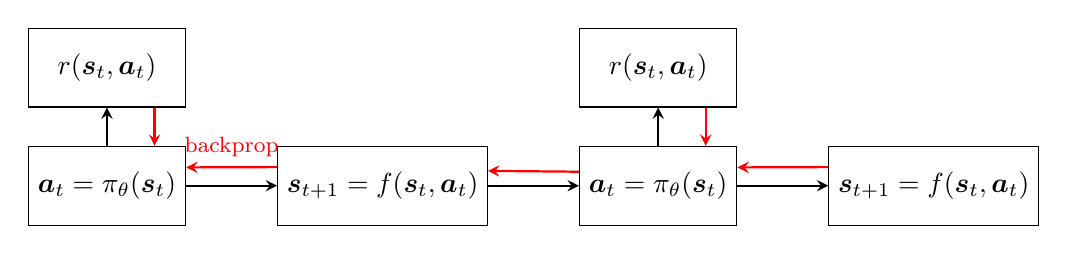
\begin{tikzpicture}[scale=1, transform shape, node distance=1.5cm]
		\node (action1) [rec] {$\bm{a}_{t} = \pi_\theta(\bm{s}_{t})$};
		\node (reward1) [rec, above of=action1] {$r (\bm{s}_{t}, \bm{a}_{t} )$};
		\draw [arrow] (action1) -- (reward1);
		\draw [arrow_red, xshift=0.5cm]  (reward1.320) -- (action1.40);
		\node (next_state1) [rec, right of=action1, xshift=2cm] {$\bm{s}_{t+1} = f (\bm{s}_{t}, \bm{a}_{t} ) $};
		\draw [arrow] (action1) -- (next_state1);
		\draw [arrow_red, xshift=0.5cm]  (next_state1.170) -- node[midway, above, color=red, font=\footnotesize] {backprop}  (action1.13);
		\node (action2) [rec, right of=next_state1, xshift=2cm] {$\bm{a}_{t} = \pi_\theta(\bm{s}_{t})$};
		\draw [arrow] (next_state1) -- (action2);
		\draw [arrow_red, xshift=0.5cm]  (action2.170) -- (next_state1.8);
		\node (reward2) [rec, above of=action2] {$r (\bm{s}_{t}, \bm{a}_{t} )$};
		\draw [arrow] (action2) -- (reward2);
		\draw [arrow_red, xshift=0.5cm]  (reward2.320) -- (action2.40);
		\node (next_state2) [rec, right of=action2, xshift=2cm] {$\bm{s}_{t+1} = f (\bm{s}_{t}, \bm{a}_{t} ) $};
		\draw [arrow] (action2) -- (next_state2);
		\draw [arrow_red, xshift=0.5cm]  (next_state2.170) -- (action2.13);
\end{tikzpicture}
\end{center}
\end{figure}
So we can just computer the derivative of the total reward w.r.t. policy parameters,
run backpropagation to find that derivative and just do gradient ascent on that derivative (in the diagram above
the red arrows are backprop arrows).
This can be easily done in Pytorch and TensorFlow.
It's easy to do for deterministic policies, but it's also possible to implement for stochastic policies.
But it is problematic.
That's because you'll get big gradients on the actions in the first timesteps and the actions on the last timestep towards the end,
due to the fact that earlier actions lead to bigger difference in the trajectories later on.
Thus the first-order methods are poorly conditioned.
There are similar parameter sensitivity probles as shooting methods. 
Also no dynamic programming is possible because the policy parameters couple all time steps.
Overall the problems are similar to those when training RNNs with very long time sequences (vanishing and exploding gradients).
However, unlike LSTMs, we can't just ``choose'' a simple dynamics to control the gradients --- nature chose our dynamics.
So all in all this is bad for model-based reinforcement learning.

\subsection{What's the solution?}
\subsubsection{First class of solutions}
Use derivative-free (model-free) RL algorithms with using the model not in the real world, but on the model to generate synthetic samples.
Altough it seems strange to use the model to train model-free algorithms, it works well in practise.
It's essentially model-based acceleration for model-free RL.
\subsubsection{Second class of solutions}
Use simpler policies than neural networks, ex. LQR with learned models (LQR-FLM (fitted local models)).
Then use those models to train local policies to solve simple(r) tasks and the combine the local policies
into a global policy via some supervised learning procedure.

\section{Model-free learning with a model}
Basically use the model-free algorithm to make use of the virtually infinite synthetic data you can get from your model.
This can be really good if, for example, you use policy gradients because the fact that you have many samples will lead to lower variance. 
The policy gradient
\begin{equation}
		\nabla_{\theta} J(\theta) \approx
		\frac{1}{N} \sum_{i=1}^{N} \sum_{t=1}^{T} \nabla_{\theta} \log \pi_\theta (\bm{a}_{i,t}| \bm{s}_{i,t}) \hat{Q}^\pi_{i,t}
\end{equation}
is also the gradient of the total reward with respect to policy parameters.
So it's also computing the derivative through the dynamics, it just doesn't require knowing the functional form of
the dynamics log probability for this.
Backprop (pathwise) gradient:
\begin{equation}
		\nabla_{\theta} J(\theta) =
		\frac{1}{N} \sum_{t=1}^{T} \frac{dr_t}{d\bm{s}_{t}} \prod_{t'=2}^{t} \frac{d\bm{s}_{t'}}{d\bm{a}_{t'-1}} \frac{d\bm{a}_{t'-1}}{d\bm{s}_{t'-1}}  
\end{equation}
Thus there 2 gradients represent the same quantity.
So policy gradient might be more stable (if enough samples are used) because it does not require multiplying many Jacobians.

\subsection{Dyna}
Let's first cover the original method from Sutton's paper.
It's an iterative online procedure.
\begin{enumerate}
		\item given state $s$, pick action $a$ using exploration policy
		\item observe $s'$ and $r$ to get transition $(s,a,s',r) $
		\item update model $\hat{p}(s'|s,a)$ and $\hat(s,a)$ using $(s,a,s')$
		\item Q-update: $Q(s,a) \leftarrow Q(s,a) + \alpha E_{s',r} \left[ r+ \max_{a'} Q(s',a') - Q(s,a) \right] $
		\item repeat $K$ times:
		\item sample $(s,a) \sim \mathcal{B}$ from buffer of past states and actions
		\item Q-update: $Q(s,a) \leftarrow Q(s,a) + \alpha E_{s',r} \left[ r+ \max_{a'} Q(s',a') - Q(s,a) \right] $. after $K $ repetitions go
				collect more samples
\end{enumerate}
The original version suggests you take an action from the dataset, but it makes more sense take actions from a new policy.
And this is how modern versions do this.

\subsubsection{General ``Dyna-style'' model-based RL recipe}
\begin{enumerate}
		\item collect some data, constisting of transitions $(s,a,s',r)$
		\item use that data to learn a model $\hat{p}(s'|s,a)$ (using whatever supervise learning technique), 
		and also learn the reward model $\hat{r}(s,a)$ if you don't know it
\item repeat $K$ times:
\item sample $s \sim \mathcal{B}$ from buffer
\item choose action $a$ (from $\mathcal{B}$ (bad part: closer to the dataset distribution), 
		from $\pi$ (bad part: incurs distributional shift in model) , or random (bad 'cos it's random)
\item simulate $s' \sim \hat{p}(s'|s,a)$ (and r = $\hat{r}(s,a)$ if needed)
\item train on $(s,a,s',r)$ with model-free RL (everything but MC policy gradients works well)
\item (optional) take $N$ more model-based steps
\end{enumerate}
The advantages are: that only short rollouts are required (as few as one step). 
This is good because distributional shift gets higher the longer the rollout is.
You get to see diverse states.
There are 3 algorithms which use this (sorted by age): 
\begin{itemize}
		\item model-based acceleration (MBA)
		\item model-based value expansion (MVE)
		\item model-based policy optimiation (MBPO)
\end{itemize}
Here's the model ML-y version of the algorithm:
\begin{enumerate}
		\item take some action $\bm{a}_{i}$ and observe $ \left( \bm{s}_{i}, \bm{a}_{i}, \bm{s}_{i}', r_i \right)   $ and add it to $ \mathcal{B}  $
		\item sample mini-batch $ \left\{  \bm{s}_{j}, \bm{a}_{j}, \bm{s}_{j}', r_j \right\}   $ uniformly
		\item use  $ \left\{  \bm{s}_{j}, \bm{a}_{j}, \bm{s}_{j}' \right\}   $ to update model $\hat{p} (\bm{s}_{}'|\bm{s}_{},\bm{a}_{})$
		\item sample $\left\{ \bm{s}_{j} \right\} $ from $ \mathcal{B}  $
		\item for each $\bm{s}_{j}$, perform model-based rollout with $\bm{a}_{} = \pi(\bm{s})$
		\item use all transtitions $ \left( \bm{s}_{}, \bm{a}_{}, \bm{s}_{}', r \right)   $ along rollout to update Q-function
\end{enumerate}

\subsection{Local models}
Super interesting actually, but will skip atm

\chapter{Exploration algorithms}
Skipped writing about bandits, but the point is that you can get provably correct (Bayesian based) strategies only in the simplest settings,
and even then stuff's intractable. But they do provide boudaries the effectiveness of much simpler strategies, which is useful for us.
Also, thankfully, the simpler strategies work quite well. We'll discuss some now.

\subsection{Optimistic exploration}
Keep track of average reward $\hat{\mu}_a$ for each action $a$.
For exploitation pick $a = \argmax \hat{\mu}_a$.
The optimistic estimate is $a = \argmax \hat{\mu}_a + C \sigma_a$,
where $C \sigma_a$ is some sort of variance estimate.
The idea is to try something until you are sure it's not great.
In the bandit case, try each arm until you're sure it's not great.
For example, do 
\begin{equation}
		a = \argmax \hat{\mu}_a + \sqrt{ \frac{2 \ln T}{N(a)} }
\end{equation}
where $N(a)$ is the number of times you picked that action.
With this algorithm, you get $\text{Reg}(T)$ to be $O(\log T)$, which is provably as good as any algorithm.
However, it's not the best in practise.

\subsection{Probability matching/posterior sampling}
Assume $ r(a_i) \sim p_{\theta_i} (r_i)  $. This defines POMDP with $ \bm{s}_{} = \left[ \theta_1, \dots, \theta_n \right]   $.
The belief state is $\hat{p}(\theta_1, \dots, \theta_n)$, i.e. this is a \textit{model} of our bandit.
The idea is to sample $ \theta_1, \dots, \theta_n  \sim \hat{p}(\theta_1, \dots, \theta_n)$. Pretend
the model $   \theta_1, \dots, \theta_n$ is correct and take the optimal action.
Then you update the model and repeat.
This is called posterior or Thompson sampling and it's kind greedy.
It's harder to analyze theoretically, but can work very well empirically.

\subsection{Information gain}
This is based on Bayesian experimental design.
Say we want to determine some latent variable $z$. Which action do we take?
Let $\mathcal{H}(\hat{p}(z))$ be the current entropy of our $z$ estimate.
Let $ \mathcal{H}(\hat{p}(z)|y)  $ be the entropy of our $z$ estimate after observation $y$ (e.g. $y$ can be $r(a)$).
The lower the entropy, the more precisely we know $z$.
Thus the information gain is:
\begin{equation}
		IG(z, y) = E_y \left[ \mathcal{H}(\hat{p}(z) - \mathcal{H}(\hat{p}(z)|y) \right] 
\end{equation}
This will then quantify how much we want to observe $y$.
It typically depends on an action, so we have $IG(z,y|a)$.
Hence we are estimating how much we learn about $z$ from action $a$, given our current belifs:
\begin{equation}
		IG(z, y|a) = E_y \left[ \mathcal{H}(\hat{p}(z) - \mathcal{H}(\hat{p}(z)|y)|a \right] 
\end{equation}

This is used in a Russo \& Van Roy paper ``Learning to optimize via information-directed sampling''.
The algorithm they use is the following one. Let $y=r_a$, $ z = \theta_a  $ (parameters of model $p(r_a)$).
Let $g(a) = IG(\theta_a, r_a|a)$  be the information gain of $a$. Further, let
$\Delta(a) = E \left[ r(a^\star) - r(a) \right] $ be the expected suboptimality of $a$.
Then choose $a$ according to $ \argmin_a \frac{\Delta (a)^2}{g(a)}   $.
Here $g(a)$ in the denominator tells to not bother with taking actions if you won't learn anything
and $\Delta (a)^2$ tells to not take actions that you're sure are suboptimal.

\subsection{General themes}
Upper confidence bound (UCB) or optimistic exploration :
\begin{equation}
		a = \argmax \hat{\mu}_a + \sqrt{ \frac{2\ln T}{N(a)}  }
\end{equation}
Thompson sampling:
\begin{gather}
		\theta_1, \dots, \theta_n \sim \hat{p} 	(\theta_1, \dots, \theta_n) \\
		a = \argmax_a E_{\theta_a} \left[ r(a) \right] 
\end{gather}
Information gain:
\begin{equation}
		IG(z,y|a)
\end{equation}
Most exploration strategies require some kind of uncertainty estimate (even if it's naive (like UCB)).
They usually assume some value to new information:
UCB assumes unknown = good (optimism), assuming that sample = truth (Thompson sampling) or
assuming that information gain = good (information gain).
These assumptions seem arbitrary, but in tractable bandit settings they are provably good.

The reason we care about bandits is because they are easier to analyze and understand and
we can use that to derive foundations for exploration methods and apply them in more complicated settings.
We didn't cover contextual bandits (bandits with state), optimal exploration in small MDPs,
Bayesian model-based reinforcement learning (similar to information gain) and probably approximately correct (PAC) exploration.
That goes more into the theory.

\section{Exploration in deep reinforcement learning}
We now carry over the exploration methods we talked about in the bandit case over to the DRL case.
How can we use UCB in RL?
Do count-based exploration:
use $N\left( \bm{s}_{}, \bm{a}_{} \right)$ or $N(\bm{s}_{})$ to add \textit{exploration bonus}.
Use $ r^+ (\bm{s}_{}, \bm{a}_{}) = r(\bm{s}_{}, \bm{a}_{}) + \mathcal{B} (N(\bm{s}_{}))  $,
where $\mathcal{B}(N(\bm{s}_{}))$ should decrease with $N(\bm{s}_{})$.
This is a simple addition to any RL algorithm. The drawback is the fact that you need to tune the bonus weight and how to do the counting.
How do you even do counting in complex MDPs? Consider Montezuma's revenge. 
You get a combinatorial explosion of states for de facto equivalent states (the skull moves, the guy moves a bit,
it's all the same but it's not the same exact state).
So we need so density model to patch these similar states together.
\subsection{Fitting generative models}
The idea is to fit a density model $ p_\theta(\bm{s}_{})  $ or $ p_\theta (\bm{s}_{}, \bm{a}_{})  $.
As mentioned, we don't want to have high $ p_\theta(\bm{s}_{})  $ for similar states.
Could we use it as a ``pseudocount''?
In small MPDs we had:
\begin{equation}
		P\left( \bm{s}_{} \right) = \frac{N(\bm{s}_{}) \leftarrow \text{ count of times in that state}}{n \leftarrow \text{ total states visited}} 
\end{equation}
and after seeing $ \bm{s}_{}  $again, we have:
\begin{equation}
		P'\left( \bm{s}_{} \right) = \frac{N(\bm{s}_{}) +1 }{n  +1 } 
\end{equation}
can we get $ p_\theta(\bm{s}_{})  $ and $ p_{\theta'}(\bm{s}_{})  $ to obey these equations?
The algorithm would go like this:
\begin{enumerate}
		\item fit model $ p_{\theta}(\bm{s}_{})  $ to all states $ \mathcal{D}  $seen so far
		\item take a step $i$ and observe $ \bm{s}_{i}  $
		\item fit new model $ p_{\theta'}(\bm{s}_{})  $ to $ \mathcal{D}  \cup \bm{s}_{i}$ 
		\item use $ p_{\theta}(\bm{s}_{i})  $ and $ p_{\theta'}(\bm{s}_{i})  $ to estimate $ \hat{N}(\bm{s}_{})  $
		\item set $ r^+_i = r_i + \mathcal{B}(\hat{N}(\bm{s}_{}))  $
\end{enumerate}
How do we $ \hat{ N}(\bm{s}_{})$?
Use:
\begin{gather}
		p_\theta(\bm{s}_{i}) = \frac{\hat{N}(\bm{s}_{i})}{\hat{n}} \\
		p_{\theta'}(\bm{s}_{i}) = \frac{\hat{N}(\bm{s}_{i})+1}{\hat{n}+1} 
\end{gather}

We have 2 equations and 2 unknowns, so:
\begin{gather}
		\hat{N}(\bm{s}_{i}) = \hat{n}p_{\theta}(\bm{s}_{i}) \\
		\hat{n} = \frac{1 - p_{\theta'}(\bm{s}_{i})}{p_{\theta'}(\bm{s}_{i}) - p_{\theta}(\bm{s}_{i})} p_{\theta}(\bm{s}_{i})
\end{gather}

\subsection{What kind of bonus to use?}
Also, what density to use?
There are a lot of functions in the literature, check slides, whatever.

\subsubsection{What kind of model to use?}
Don't really need to sample from it, doesn't really need to be normalized either (so no need for GANs or VAEs).
You just want the output densities. 
Some papers use CTS, stochastic neural networks, compression length, EX2 (whatever).
Then Sergey goes over papers which use these, don't really need those details here.

Here I skipped writting about lec13-part4..

\section{Posterior sampling in deep RL}
Let's refresh Thompson sampling so that we can make an analog in MDPs:
\begin{gather}
		\theta_1, \dots, \theta_n \sim \hat{p} (\theta_1, \dots, \theta_n) \\
		a = \argmax_a E_{\theta_a} \left[ r(a) \right] 
\end{gather}
In the bandit setting $ \hat{p}(\theta_1, \dots, \theta_n)  $ is the distribution over rewards.
The MDP analog is the Q-function as in DRL we choose an action as the argmax of the Q-function.
So for example we could do:
\begin{enumerate}
		\item sample Q-function $Q$ from $p(Q)$
		\item act according to $Q$ for one episode
		\item update $p(Q)$ and repeat from 1.
\end{enumerate}
Since Q-learning is off-policy, we don't care which Q-function was used to collect data.

How do we represent a distribution over function?
We could try using bootstrap ensembles.
So, given a dataset $\mathcal{D}$, resample with replacement $N$ times to get $\mathcal{D}_1, \dots, \mathcal{D}_N$.
Then train each model $f_{\theta_i}$ on $ \mathcal{D}_i  $.
To sample from $ p(\theta)  $, sample $ i \in [1, \dots, N]  $ and use $ f_{\theta_i}  $.
Training $N$ big neural nets is expensive, and we again solve this the same way we did it MBRL.

This works becuase a random Q-function is more likely to be consistent in what it's doing than
standard $\epsilon$-greedy exploration. But it's still not particularly good.

\section{Information gain in DRL}
It's $ IG(z,y|a)  $. But it's information about what?
Information about the reward $ r(\bm{s}_{}, \bm{a}_{})  $ is not very useful if the reward is sparse.
Information about state density $ p(\bm{s}_{})  $ would make sense because it tells us about changing state density (and thus tells about novelty).
We could do information about dynamics $ p(\bm{s}_{}'|\bm{s}_{}, \bm{a}_{})  $ and that would be a good proxy for \textit{learning} the MDP, but 
it would still be heuristic.
Regardless of what we're estimating, information gain's generally intractable to be used exactly.
So let's talk about the approximations we could make.
One thing is prediction gain: $ \log p_{\theta'}(\bm{s}_{}) - \log p_\theta(\bm{s}_{})  $.
Intuitively, if density changes a lot, the state would be novel. So we could use this in
a manner similar to pseudocounts.
We could do variational inference. This is because IG can be equivalently written as $ D_{KL} \left( p(z|y)||p(z) \right)   $.
We learn about \textit{transitions} $ p_\theta (s_{t+1}|s_t, a_t): z = \theta  $. $z$ is what we care about.
We try to find transitions $ y = \left( s_t, a_t, s_{t+1} \right)   $ which are most informative about $\theta$.
Then we want to maximize $ D_{KL} \left( p(\theta|h, s_t, a_t, s_{t+1})||p(\theta|h) \right)   $,
where $\theta$ are the model parameters for $ p_\theta (s_{t+1}|s_t, a_t)  $,
$h$ is the history of all prior transitions and $ \left( s_t, a_t, s_{t+1} \right)   $ is the newly
observed transition.
The intuition is that a transition is more informative if it causes belief over $\theta$ to change.
We can't get the true posterior of course.
But we can, for example, use variational inference to estimate $ q(\theta|\phi) \approx p(\theta|h)  $.
Then, given a new transition $ \left( s,a,s' \right)   $ we update $\phi$ to get $ \phi'  $.
This is called VIME. Specifically, we optimize the variational lower bound
$ D_{KL}(q(\theta|\phi)||p(h|\theta)p(\theta)  $ .
We represent $ q(\theta|\phi)  $ as a product of independent Gaussian parameter distributions with mean $ \phi  $,
i.e. we use $ p(\theta|\mathcal{D}) = \prod_{i}^{}p(\theta_i|\mathcal{D})   $,
where $ p(\theta_i|\mathcal{D}) = \mathcal{N}(\mu_i, \sigma_i)  $, where $\phi$ can be the mean, or 
the mean and the variance (if it's just the mean, the variance is constant).
The, given the new transition $ \left( s,a,s' \right)   $ we update $ \phi  $ to get $ \phi'  $,
i.e. we update the network means and variances.
We use $ D_{KL}(q(\theta|\phi')||q(\theta|\phi))  $ as approximate bonus.
The plus of all this is the appealing mathematical formalism, but the minus is that
the models are more complex and generally harder to use effectively.

\section{Exploration with model errors}
$ D_{KL}(q(\theta|\phi')||q(\theta|\phi))  $ can be seen as change in the network (mean) parameters $ \phi  $.
If we forget about IG, there are many other ways to measure this,
for example using an autoencoder to get a latent space representation and the using the autoencoder
loss as an exploration bonus.
Using errors and models as an exploration bonus is a heavily studied area even though it's
not always tied to information gain.

\section{Unsupervised exploration}
We'll use information theory for this.
The idea is to learn about the world without an explicit goal.
Let's set the notation first.
The distribution over states (or observations) is:
\begin{equation}
		p(\bm{x}_{})
\end{equation}
The entropy of $ p(\bm{x}_{})  $is:
\begin{equation}
		\mathcal{H}(p(\bm{x}_{})) = - E_{\bm{x}_{} \sim p(\bm{x}_{})} \left[ \log p(\bm{x}_{}) \right] 
\end{equation}
Intuitively, entropy is the width of the distribution.
Mutual information is defined as:
\begin{align}
		\mathcal{I}(\bm{x}_{};\bm{y}_{}) &= D_{KL}(p(\bm{x}_{}, \bm{y}_{})||p(\bm{x}_{})p(\bm{y}_{})) \\
										 &=
		E_{(\bm{x}_{}, \bm{y}_{}) \sim p(\bm{x}_{}, \bm{y}_{})}  \left[ \log \frac{p(\bm{x}_{},\bm{y}_{})}{p(\bm{x}_{})p(\bm{y}_{})}  \right] \\
 &= \mathcal{H}(p(\bm{y}_{})) - \mathcal{H}(p(\bm{y}_{}|\bm{x}_{}))
\end{align}

\subsection{Information theoretic quantities in RL}
The state \textit{marginal} distribution of policy $ \pi  $:
\begin{equation}
		\pi(\bm{s}_{})
\end{equation}
The state \textit{marginal} entropy of policy $ \pi  $ is:
\begin{equation}
		\mathcal{H}\pi(\bm{s}_{})
\end{equation}
It quantifies coverage that the policy gets.
This can come in, for example, the following setting.
``Empowerement'' is defined as the mutual information between the next state and the current action:
\begin{equation}
		\mathcal{I}(\bm{s}_{t+1}; \bm{a}_{t}) = 
		\mathcal{H}(\bm{s}_{t+1}) - \mathcal{H}(\bm{s}_{t+1}|\bm{a}_{t})
\end{equation}

\chapter{Unsupervised reinforcement learning (sketches)}
Let's say you have a generative model. Then
you can sample from it and make the sample be a goal.
Then use the data you gather to improve both the policy and the model.
A sketch of that algorithm would look something like this:
\begin{enumerate}
		\item propose goal: $ z_g \sim p(z), x_g \sim p_\theta (x_g|z_g)  $
		\item attempt to reach goal using $ \pi(a|x,x_g)  $, reach $ \bar{x}  $
		\item use data to update $ \pi  $
		\item use data to update $ p_\theta(x_g|z_g), q_\phi(z_g|x_g)  $
\end{enumerate}

But since the generative model is trained on the data it has seen,
it will generate data similar to what it has seen!
So this is bad for exploration.
To ameliorate this, you could replace the standard maximum likelihood estimation (MLE):
\begin{equation}
		\theta, \phi \leftarrow \argmax_{\theta, \phi} E \left[ \log p(\bar{x}) \right] 
\end{equation}
with a weighted MLE:
\begin{equation}
		\theta, \phi \leftarrow \argmax_{\theta, \phi} E \left[ w(\bar{x}) \log p(\bar{x}) \right] 
\end{equation}

The gerative model should be able to give us a density score:
\begin{equation}
		w(\bar{x}) = p_\theta(\bar{x})^\alpha
\end{equation}
where $ \alpha \in [-1,0>  $.
Then $ \mathcal{H}(p_\theta(x))  $ will increase!
In the limit we'll get a uniform distribution over valid states.
So we'll get nice diverse goals with this scheme.

But what's the objective of this scheme (what are we maximizing)?
Well, we'll maximizing $ \max \mathcal{H}(p(G))  $.
The RL is trying to train $ \pi(a|S,G)  $ to reach $ G  $.
This means that $ p(G|S)  $ becomes more deterministic.
Thus our policy is capable to deterministically reach it's goal,
i.e. the better the policy is, the easier it is to predict $G$ from $S$.
So we're doing:
\begin{equation}
		\max \mathcal{H}(p(G)) - \mathcal{H}(p(G|S)) = \max \mathcal{I}(S;G)
\end{equation}
In short, maximizing the mutual information between $ S  $ and $ G  $ leads to
good exploration $ \mathcal{H}(p(G))  $ and effective goal reaching $\mathcal{H}(p(G|S))  $

\subsection{Aside: exploration with intrinsic motivation}
Just doing some form of pseudocounting to incentivise exploration won't cut it.
Imagine the followign procedure:
\begin{enumerate}
		\item update $ \pi(\bm{a}_{}|\bm{s}_{})  $ to maximize $ E_\pi \left[ \tilde{r}(\bm{s}_{}) \right]   $
		\item update $ p_\pi(\bm{s}_{})  $ to fit the state marginal and repeat.
\end{enumerate}
If there's no reward at all, the density estimator will fit whatever the policy did,
the policy will do something else, and so on.
While (the state density estimator will be good,
The policy you'll end up with will be some arbitrary mess.
Let's construct the reward
\begin{equation}
		\tilde{r}(\bm{s}_{}) = \log p^\star (\bm{s}_{}) - \log p_\pi (\bm{s}_{})
\end{equation}
The RL algorithm is not aware that the reward depends on the policy.
So this won't perform marginal matching --- 
the policy will jump around the state space and that's all it'll do.
Let's sketch the algorithm out anyway, fixing it will be later then:
\begin{enumerate}
		\item learn $ \pi^k (\bm{a}_{}|\bm{s}_{})  $ to maximize $ E_\pi \left[ \tilde{r}^k(\bm{s}_{}) \right]   $
		\item update $ p_{\pi^k}(\bm{s}_{})  $ to fit the state marginal
\end{enumerate}
To fix this we should change 2. to
update $ p_{\pi^k}(\bm{s}_{})  $ to fit \textit{all states seen so far}.
Another change is to return a mixture policy $ \pi^\star (\bm{a}_{}|\bm{s}_{})  = \sum_{k}^{} \pi^k(\bm{a}_{}|\bm{s}_{}) $
instead of the latest policy.
This mixture is a mixture model of all the policies seen so far.
So you'll choose a random policy you've seen during learning.
We do this because we then do perform marginal matching.
To explain this we need a bit of game theory.
Namely,
\begin{equation}
		p_\pi(\bm{s}_{}) = p^\star (\bm{s}_{}) 
\end{equation}
is the Nash equilibrium of a two player game.
The players are the state density estimator $ p_{\pi^k}  $and the policy $\pi^k$.
The way to reach the algorithm is to start anywhere and always play best responce,
which for the density mathing is to actually fit the density an for the policy
it is to maximize $ \tilde{r}  $.
But just doing this won't yield the mixed Nash equilibrium --- the average over all
of the final results of the game will thought.
And that's why we're averaging the mixture.

\section{Learning diverse skills}
Let's say you have $n$ policies for $n$ skills.
Most generally you could have:
\begin{equation}
		\pi(\bm{a}_{}|\bm{s}_{},z)
\end{equation}
i.e. a policy conditioned on $z$ which denotes the task index.
However, reaching diverse \textbf{goals} is not the same as performing diverse \textbf{tasks}
and not all behaviors can be captured by \textbf{goal-reaching}.
The intuition is that different \textbf{skills} should visit different \textbf{state-space regions}.

\subsection{Diversity-promoting reward function}
\begin{equation}
		\pi(\bm{a}_{}|\bm{s}_{},z) = \argmax_\pi \sum_{z}^{} E_{\bm{s}_{} \sim \pi(\bm{s}_{}|z)} \left[ r(\bm{s}_{},z) \right] 
\end{equation}
With this you can reward states that are unlikely for other $ z' \neq z  $.
One way to do this is to have the reward function be a classifier which tries to see which $z$ you're doing
based on which state you're in, ex:
\begin{equation}
		r(\bm{s}_{}, z) = \log p(z|\bm{s}_{})
\end{equation}
There's a connection to mutual information:
\begin{equation}
		I(z, \bm{s}_{}) = H(z) - H(z|\bm{s}_{})
\end{equation}
which is again maximized here
because $H(z)$ is maximized by using a uniform prior and 
$H(z|s)$ is minimized by maximizing $\log p(z|\bm{s}_{})$.

\chapter{Generalisation gap}
RL methods do not generalize as well as supervised learning techniques.
Maybe we need more scaling and more variety in data?
The problem is we're doing fundametally online learning (be it on or off policy).
\subsubsection{What makes modern machine learning work}
Data.
So can we develop data-driven RL methods?
Enter off-policy reinforcement learning.
The idea is that some policy collected the data beforehand.
Would be cool if we could gather data once with some policy and then reuse it, otherwise we're stuck
with needed to generate our own data every time.

Let's formalize offline RL. First let's get some notation:
\begin{itemize}
		\item dataset: $ \mathcal{D} = \left\{ \left( \bm{s}_{i}, \bm{a}_{i}, \bm{s}_{i}', r_i \right)  \right\}   $
		\item states: $ \bm{s}_{} \sim d^{\pi \beta}(\bm{s}_{})  $
		\item actions $ \bm{a}_{} \sim \pi_\beta(\bm{a}_{}|\bm{s}_{})$
		\item next states: $ \bm{s}_{}' \sim p(\bm{s}_{}'|\bm{s}_{}, \bm{a}_{})$
		\item rewards: $r \leftarrow r(\bm{s}_{}, \bm{a}_{})$
\end{itemize}
and the RL objective is:
\begin{equation}
		\max_\pi \sum_{t=0}^{T} E_{\bm{s}_{t} \sim d^\pi(\bm{s}_{}), \bm{a}_{t} \sim \pi(\bm{a}_{}|\bm{s}_{})} \left[ \gamma^t r (\bm{s}_{t}, \bm{a}_{t} ) \right] 
\end{equation}

Let's talk about off-policy evaluation.
Given $ \mathcal{D} $, estimate $ J(\pi) = E_{\pi} \left( \sum_{t=1}^{T} r (\bm{s}_{t}, \bm{a}_{t} ) \right)  $.
Offine reinforcement learning, also called batch RL and sometimes fully off-policy RL.
Given $ \mathcal{D} $, learn the best possible policy $ \pi_\theta $.
This is not the best possible policy for the MDP, but the best policy given your dataset.

What should a good offline RL algorithm do?
\begin{enumerate}
		\item find the ``good stuff'' in a dataset with both good and bad behaviors
		\item generalize --- realize that good behavior in one place may also be good in another place
		\item do ``stiching'' --- combine parts of good behaviors into a superior behavior 
				(if one goes from A to B well and another from B to C, combine into optimal path from A to C)
\end{enumerate}

What do we expect offline RL methods to do?
Not do imitation learning! It should be provably better.
Instead, it should be able to extract order from chaos by stiching and generalizing.
Thus it should be able to achieve amazing performance even from poor data.

An example: have data of a robot that pick an object from a drawer and open a drawer.
Ask it to do both even if it has never seen that before and it should be able to do so.
This is superior to standard RL where the policy only works from known starting states.

\subsection{Why is offline RL hard?}
There's a fundametal problem of counterfactual queries.
Say a policy generates some action which wasn't in the dataset.
We have no way of knowing wether it's good or bad. In online RL,
the policy would try that action, see that it was bad, and never repeat it again.
But we'd like offline RL methods to somehow account for these unseen
``out-of-distribution'' actions, ideally in a safe way.
And we'd still like the generalization to happen!
So it's a complicated tradeoff.
In statistics this is called \textbf{distribution shift},
i.e. the problem of training under one distribution and need to perform under another distribution,
leading to bad performance.
For example, let's say you're doing supervised learning:
\begin{equation}
		\theta \leftarrow \argmin_\theta E_{\bm{x}_{} \sim p(\bm{x}_{}), y \sim p(y|\bm{x}_{})} 
		\left[ (f_\theta(\bm{x}_{}) - y)^2 \right] 
\end{equation}
where $y  $ is the ground truth we're regressing onto.
The examples come from $ p(\bm{x}_{}) $ and $y$s come from $ p(y|\bm{x}) $.
This is called empirical risk minimization (ERM)
 (the given equation is the actual risk).

 Question: given some $ \bm{x}_{}^\star $, is $ f_\theta(\bm{x}_{}^\star )$ correct?
 Well, if you didn't overfit,
 \begin{equation}
E_{\bm{x}_{} \sim p(\bm{x}_{}), y \sim p(y|\bm{x}_{})} 
		\left[ (f_\theta(\bm{x}_{}) - y)^2 \right]
\end{equation} 
is low.
But 
\begin{equation}
   	 E_{\bm{x}_{} \sim \bar{p}(\bm{x}_{}), y \sim p(y|\bm{x}_{})} 
   	\left[ (f_\theta(\bm{x}_{}) - y)^2 \right]
\end{equation} 
is not for general $ \bar{p}(\bm{x}) \neq p(\bm{x}_{}) $.
What if $ \bm{x}_{}^\star \sim p(\bm{x}_{}) $?
Not necessarily.
But shouldn't neural networks generalize and overcome this problem?
That could happen, but if
$ \bm{x}_{}^\star \leftarrow \argmax_{\bm{x}} f_\theta(\bm{x}_{}) $?
Well then we have a problem.
This is what happens with adversarial examples.

\subsection{Where does RL suffer from distributional shift?}
Let's look at Q-learning:
\begin{equation}
		Q (\bm{s}_{}, \bm{a}_{} ) \leftarrow
		r (\bm{s}_{}, \bm{a}_{} ) + \max_{\bm{a}_{}'} Q (\bm{s}_{}', \bm{a}_{}' )
\end{equation}
we could equivalently write this as:
\begin{equation}
		Q (\bm{s}_{}, \bm{a}_{} ) \leftarrow
		\underbrace{r (\bm{s}_{}, \bm{a}_{} ) + E_{\bm{a}_{}' \sim \pi_{\text{new}}} \left[    Q (\bm{s}_{}', \bm{a}_{}' )\right]}_{y (\bm{s}_{}, \bm{a}_{} )}
\end{equation}
So the objective is:
\begin{equation}
	\min_{Q} E_{(\bm{s}_{}, \bm{a}_{} )\sim \pi_{\beta}(\bm{s}_{}, \bm{a}_{} )}
	\left[ \left( Q (\bm{s}_{}, \bm{a}_{} ) - y (\bm{s}_{}, \bm{a}_{} ) \right)^{2}  \right] 
\end{equation}
where $ \pi_{\beta}  $ is the behavioral policy and
$ y (\bm{s}_{}, \bm{a}_{} ) $ is the target value.
We expect good accuracy when $ \pi_{\beta} (\bm{a}_{}|\bm{s}_{}) = \pi_{\text{new}} (\bm{a}_{}|\bm{s}_{})  $.
But that's not going to happen because we want $ \pi_{\text{new}}  $
to be better.
Even worse,
\begin{equation}
		\pi_{\text{new}} = \argmax_{\pi} E_{\bm{a}_{}\sim p(\bm{a}_{}|\bm{s}_{}) } \left[ Q (\bm{s}_{}, \bm{a}_{} ) \right] 
\end{equation}
so we exactly have distributional shift.
We are explicity finding adversarial examples when training $ \pi_{\text{new}}  $
Furthermore, the issues with generalization which are correct in the online
setting are not correct in the offline setting.
So existing challenges with sampling error and function approximation error in standar RL
become much more severe in offline RL.

\section{Batch RL via importance sampling}
The classic, pre-deep learning offline learning methods.
Let's do what we did when we derived off-policy policy gradients.
The RL objective is:
\begin{equation}
		\max_{\pi} \sum_{t=0}^{T} E_{\bm{s}_{t}\sim d^{\pi}, \bm{a}_{t}\sim \pi (\bm{a}_{}|\bm{s}_{})}
		\left[ \gamma^{t} r (\bm{s}_{t}, \bm{a}_{t} ) \right] 
\end{equation}
The policy gradient is:
\begin{align}
		\nabla_{\theta} J(\theta) &= E_{\tau \sim \pi_{\theta}(\tau)}
\left[ \sum_{t=0}^{T} \nabla_{\theta} \gamma^{t} \log \pi_{\theta} (\bm{a}_{t}| \bm{s}_{t} ) \hat{Q} (\bm{s}_{t}, \bm{a}_{t} ) \right]  \\
  &\approx \sum_{i=1}^{N} \sum_{t=0}^{T} \nabla_{\theta} \gamma^{t} \log \pi_{\theta} (\bm{a}_{t,i}| \bm{s}_{t,i} )
  \hat{Q} (\bm{s}_{t,i}, \bm{a}_{t,i} )
\end{align}
where we can't sample from $ \pi_{\theta}  $ because we only
have samples from $ \pi_{\beta}  $ so we do importance sampling:
\begin{equation}
\nabla_{\theta} J(\theta) \approx 
\frac{1}{N} \sum_{i=1}^{N} 
\underbrace{\frac{\pi_{\theta}(\tau_i)}{\pi_\beta(\tau_i)} }_{\text{importance weight}}
\sum_{t=0}^{T} 
\nabla_{\theta} \gamma^t \log \pi_\theta (\bm{a}_{t,i}| \bm{s}_{t,i} ) \hat{Q} (\bm{s}_{t,i}, \bm{a}_{t,i} )
\end{equation}
where the problem is that
\begin{equation}
		\frac{\pi_\theta(\tau)}{\pi_\beta(\tau)} =
		\frac{\cancel{p(\bm{s}_{1}) \prod_{t}^{} p(\bm{s}_{t+1}| \bm{s}_{t}, \bm{a}_{t})} \pi_\theta (\bm{a}_{t}| \bm{s}_{t} ) }
		{\cancel{p(\bm{s}_{1}) \prod_{t}^{} p(\bm{s}_{t+1}| \bm{s}_{t}, \bm{a}_{t})} \pi_\beta (\bm{a}_{t}| \bm{s}_{t} ) } 	
\end{equation}
is exponential in T (vanishing gradient problem)
so the weights are likely to degenerate as T becomes large.
We can't fix this the same way as in off-policy RL because now $\pi_{ \beta }$ and $\pi_{ \text{new} }$ are not similar!
Let's rewrite our gradient approximation.
\begin{equation}
\nabla_{ \theta } J (\theta) \approx \frac{1}{N} \sum_{i=1}^{N} \sum_{t=0}^{T} 
\left( \prod_{t'=0}^{t-1} \frac{\pi_{ \theta } (\bm{a}_{t',i}|\bm{s}_{t',i})}{\pi_{ \beta } (\bm{a}_{t',i}|\bm{s}_{t',i})}   \right) 
\nabla_{ \theta } \gamma^{ t }  \log \pi_{ \theta } (\bm{a}_{t,i}| \bm{s}_{t,i} )
\left( \prod_{t'=t}^{T} \frac{\pi_{ \theta } (\bm{a}_{t',i}| \bm{s}_{t',i} )}{\pi_{ \beta }(\bm{a}_{t',i}| \bm{s}_{t',i} )}   \right)
\hat{Q} (\bm{s}_{t,i}, \bm{a}_{t,i} )
\end{equation}
where $ \prod_{t'=0}^{t-1} \frac{\pi_{ \theta } (\bm{a}_{t',i}|\bm{s}_{t',i})}{\pi_{ \beta } (\bm{a}_{t',i}|\bm{s}_{t',i})}  $
acocunts for the difference in probability of landing in $ \bm{s}_{t,i}  $.
We have $ \bm{s}_{t}\sim d^{ \pi_{ \beta } }  (\bm{s}_{t})$, but we want
$ \bm{s}_{t}\sim d^{ \pi_{ \theta } }  \bm{s}_{t}$.
Also, $ \prod_{t'=t}^{T} \frac{\pi_{ \theta } (\bm{a}_{t',i}| \bm{s}_{t',i} )}{\pi_{ \beta }(\bm{a}_{t',i}| \bm{s}_{t',i} )}  $
accounts for having the incorrect $ \hat{Q} (\bm{s}_{t,i}, \bm{a}_{t,i} )  $.
The classic on-policy techniques disregard the first product and
take multiple gradient steps with this gradient before gathering more data
and again this is justified because the policies $ \pi_{ \theta }  $ and $ \pi_{ \beta }  $ are similar.

In fact, it turns out that to avoid exponentially exploding importane weights,
we \textbf{must} use value function estimation!
However, we'll still discuss the approaches which don't do this (Sergey I trust you).

Let's talk about the other problematic term.
One way to estimate $ \hat{Q} (\bm{s}_{t,i}, \bm{a}_{t,i} )  $ is to just sum up the future rewards:
\begin{equation}
\hat{Q} (\bm{s}_{t,i}, \bm{a}_{t,i} ) = E_{ \pi_{ \theta } } \left[ \sum_{t'=t}^{T} \gamma^{ t'-t }r_{ t' } \right]  
\approx \sum_{t'=t}^{T} \gamma^{ t'-t }r_{ t',i }
\end{equation}
and we'd get:
\begin{equation}
		\left( 
\prod_{t'=t}^{T} \frac{\pi_{ \theta }(\bm{a}_{t',i}| \bm{s}_{t',i} )}{\pi_{ \beta }(\bm{s}_{t',i}, \bm{a}_{t',i} )}  
		\right) 
		\hat{Q}(\bm{s}_{t,i}, \bm{a}_{t,i} )
		\approx
		\sum_{t'=t}^{T} \left( \prod_{t''=t}^{T}  \frac{\pi_{ \theta }(\bm{a}_{t'',i}| \bm{s}_{t'',i} )}{\pi_{ \beta }(\bm{s}_{t'',i}, \bm{a}_{t'',i} )} \right) 
\gamma^{ t'-t } r_{ t',i }
\end{equation}
One thing that can be done here is to break up the importance weights further.
Since action in the future don't affect the actions in the past, you can sum only the action
probabilites from $ t  $ to $ t'  $, getting:
\begin{equation}
		\sum_{t'=t}^{T} \left( \prod_{t''=t}^{t'}  \frac{\pi_{ \theta }(\bm{a}_{t'',i}| \bm{s}_{t'',i} )}{\pi_{ \beta }(\bm{s}_{t'',i}, \bm{a}_{t'',i} )} \right) 
\gamma^{ t'-t } r_{ t',i }
\end{equation}
This doesn't change the complexity, but it makes things a bit better.
Another idea worth discussing is the :
\subsection{The doubly robust estimator}
This is somewhat like a baseline for importance sampling.
\begin{equation}
\hat{V}^{\pi_\theta}(\bm{s}) \approx
\sum_{t'=t}^{T} \left( \prod_{t''=t}^{t'}  \frac{\pi_{ \theta }(\bm{a}_{t'',i}| \bm{s}_{t'',i} )}{\pi_{ \beta }(\bm{s}_{t'',i}, \bm{a}_{t'',i} )} \right) 
\gamma^{ t'-t } r_{ t',i }
\end{equation}
Let's drop the indeces and continue
\begin{align}
\hat{V}^{\pi_\theta}(\bm{s}_{ 0 }) &\approx
\sum_{t=0}^{T}
\left(   
\prod_{t'=0}^{t} \frac{\pi_{ \theta  }(\bm{s}_{t'}, \bm{a}_{t'} )}{\pi_{ \beta }(\bm{s}_{t'}, \bm{a}_{t'} )}  
\right) \gamma{t}r_{ t }  \\
&= 
\sum_{t=0}^{T} \left( \prod_{t'=0}^{T} \rho_{ t' }  \right) \gamma^{ t } r_{ t } \\
&=
\rho_{ 0 }r_{ 0 } + \rho_{ 0 }\gamma \rho_{ 1 }r_{ 1 } + \rho_{ 0 }\gamma \rho_{ 1 }\gamma \rho_{ 2 }r_{ 2 } + \dots \\
&=
\rho_{ 0 } (r_{ 0 } + \gamma (\rho_{ 1 } (r_{ 1 } + \gamma )\rho_{ 2 } (r_{ 2 } + \gamma)))) \\
&=
\bar{V}^{ T } \text{where } \bar{V}^{ T+1-t } = \rho_{ t } (r_{ t } + \gamma \bar{V}^{ T-t })
\end{align}

Let's first derive doubly robust estimation in the bandit case:
\begin{equation}
		V_{ DR } (s) = \hat{V} (s) + \rho (s,a) (r_{ s,a } - \hat{Q} (s,a))
\end{equation}
where $ \hat{V}  $ and $ \hat{Q}  $ are models of function approximators.
This is done to reduce the variance of the importance estimate,
just like the baseline did.
Now we'll try to do the same to $ \bar{V}  $:
\begin{equation}
		\bar{V}^{ T+1-t }_{ DR } = \hat{V} (\bm{s}_{t}) + \rho_{ t } (r_{ t } + \gamma \bar{V}_{ DR }^{ T-t } - \hat{Q}(\bm{s}_{t}, \bm{a}_{t} ))
\end{equation}
so this is the recursive version of the bandit case.

\subsection{Marginalized importance sampling}
The main idea here is to use not the product of action probabilities $ \prod_{t}^{} \frac{\pi_{ \theta }(\bm{s}_{t}, \bm{a}_{t} )}{\pi_{ \beta }(\bm{s}_{t}, \bm{a}_{t} )}    $ , but estimate importance
weights that are estimates of state probabilities or state-action probabilities 
$ w (\bm{s}_{}, \bm{a}_{} ) = \frac{d^{ \pi_{ \theta } } (\bm{s}_{}, \bm{a}_{} )}{d^{ \pi_{ \beta } }(\bm{s}_{}, \bm{a}_{} )}  $
If we can do this, we can estimate $ J (\theta) \approx \frac{1}{N}  \sum_{i}^{} w (\bm{s}_{i}, \bm{a}_{i} )r_{ i }  $.
Typically this is done for off-policy evaluation rather than policy learning.
How do we determine $ w (\bm{s}_{}, \bm{a}_{} )  $? Typically we set and then solve some kind of consistency condition.
That would be something like a Bellman equation, but for (state of state-action) importance weights.
For example,
\begin{equation}
		\begin{split}
d^{ \pi_{ \beta } } (\bm{s}_{}', \bm{a}_{} ') w (\bm{s}_{}', \bm{a}_{}' ) =
(1 -\gamma ) p_{ 0 } (\bm{s}_{}') \pi_{ \theta } (\bm{a}_{}'| \bm{s}_{} ') +\\
\gamma \sum_{\bm{s}_{}, \bm{a}_{}}^{} \pi_{ \theta } (\bm{a}_{}'| \bm{s}_{}' ) p (\bm{s}_{}'|\bm{s}_{}, \bm{a}_{}) d^{ \pi_{ \beta } }
(\bm{s}_{}, \bm{a}_{} ) w (\bm{s}_{}, \bm{a}_{} )
		\end{split}
\end{equation}
I won't explain this in any way because why would I (Sergey why did we go into this?).

\section{Batch RL via linear fitted value functions}
We'll talk about this because the analysis in the nonlinear function approximation case will be similar
and because the linear fitted value function will have closed-form solution which can give us a hint
on how to implement new more advanced methods.

I'm skipping lecture 15 part 3 and the entire lecture 16 'cos i really don't need offline RL rith now.
I'm also skipping lecture 17, which while it looks really interesting, i don't need right now (RL theory, bounds on things etc).
And i'm also skipping lecture 18 in the hope that i won't need variational inference to read the next 2 papers,
altough i'll certainly need this later.

\chapter{Reinforcement learning as an inference problem}
In which we look to something other than reinforcement learning and optimal control to
provide a reasonable model of human behavior.
We also try to derive optimal control, RL and planning as \textit{probabilistic inference}.

\section{Optimal control as a model of human behavior}
Let's assume a person does this:
\begin{align}
\bm{a}_{1}, \dots, \bm{a}_{T} &= \argmax_{\bm{a}_{1}, \dots, \bm{a}_{T}} \sum_{t=1}^{T} r (\bm{s}_{t}, \bm{a}_{t} ) \\
\bm{s}_{t+1} &= f (\bm{s}_{t}, \bm{a}_{t} ) \\
\pi &= \argmax_{\pi} E_{ \bm{s}_{t+1} \sim p (\bm{s}_{t+1} | \bm{s}_{t}, \bm{a}_{t}), \bm{a}_{t} \sim \pi (\bm{a}_{t}| \bm{s}_{t} ) } \left[ r (\bm{s}_{t}, \bm{a}_{t} ) \right] \\
\bm{a}_{t} &\sim \pi (\bm{a}_{t}| \bm{s}_{t} )
\end{align}
where optimizing $ r (\bm{s}_{t}, \bm{a}_{t} )  $ explains the data  (human behavior).
But what if the data is not optimal? 
Often, humans and monkeys don't care about perfection, especially when perfection does not make
much of a difference.
Some mistakes matter more than other and behavior is stochastic, but good behavior is still most likely.
In fact, we can prove that in all fully observable settings, a deterministic policy will be optimal.

Now we'll derive probabilistic policies tho and they'll look more like behaviors we observe in animals.
\begin{equation}
		\underbrace{p (\bm{s}_{1:T}, \bm{a}_{1:T})}_{ \tau } = ?
\end{equation}
We'll introduce binary variables which tell us whether the behavior we're observing is optimal or not.
The Markov chain which is our model then looks like:
\begin{figure}[htpb]
\begin{center}
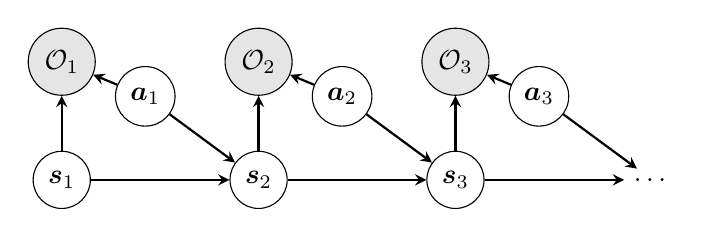
\begin{tikzpicture}[scale=1, transform shape, node distance=1.5cm]
		\node (s1) [mcs] {$\bm{s}_{1} $};
		\node (o1) [mcsb, above of=s1] {$\mathcal{O}_{ 1 }$};
		\draw [arrow] (s1) -- (o1);
		\node (a1) [mcs, above right of=s1] { $ \bm{a}_{1}  $};
		\draw [arrow] (a1) -- (o1);
		\node (s2) [mcs, right of=s1, xshift=1cm] { $ \bm{s}_{2}  $};
		\node (o2) [mcsb, above of=s2] {$\mathcal{O}_{ 2 }$};
		\draw [arrow] (s1) -- (s2);
		\draw [arrow] (a1) -- (s2);
		\draw [arrow] (s2) -- (o2);
		\node (a2) [mcs, above right of=s2] { $ \bm{a}_{2}  $};
		\draw [arrow] (a2) -- (o2);
		\node (s3) [mcs, right of=s2, xshift=1cm] { $ \bm{s}_{3}  $};
		\draw [arrow] (a2) -- (s3);
		\draw [arrow] (s2) -- (s3);
		\node (o3) [mcsb, above of=s3] {$\mathcal{O}_{ 3 }$};
		\node (a3) [mcs, above right of=s3] { $ \bm{a}_{3}  $};
		\draw [arrow] (s3) -- (o3);
		\draw [arrow] (a3) -- (o3);
		\node (s4) [right of=s3, xshift=1cm] {$\dots$};
		\draw [arrow] (s3) -- (s4);
		\draw [arrow] (a3) -- (s4);
\end{tikzpicture}
\end{center}
\end{figure}

Then the inference problem we're trying to solve is
\begin{equation}
		p (\tau | \mathcal{O}_{ 1:T })
\end{equation}
and we'll choose the following form for the distribution:
\begin{equation}
		p (\mathcal{O}| \bm{s}_{t}, \bm{a}_{t}) = \exp (r (\bm{s}_{t}, \bm{a}_{t} ))
\end{equation}
for this we'll need all the rewards to be negative, which is no problem because optimal 
behavior is invariant to additive change (unless rewards are unbounded, but we don't deal with that anyway).
With this we have:
\begin{align}
p (\tau| \mathcal{O}_{ 1:T }) &= \frac{p (\tau, \mathcal{O}_{ 1:T })}{p (\mathcal{O}_{ 1:T })} \\
&\propto p (\tau) \prod_{t}^{} \exp (r(\bm{s}_{t}, \bm{a}_{t} ))\\ 
&= p (\tau) \exp \left( \sum_{t}^{} r (\bm{s}_{t}, \bm{a}_{t} ) \right)  
\end{align}
The maximum reward trajectory will be most likely and the other rewards will be exponentially less likely.
This looks like monkeys reaching bananas on a screen (running example for realistic animal behavior).

So the cool thing is we can model suboptimal behavior (important for inverse RL).
We can apply inference algorithms to solve control and planning problems.
This provides an explanation for why stochastic behavior might be preferred (useful for exploration and transfer learning).

How do we do inference in this model?

\section{Control as inference}
We are interested in the following 3 inference problems:
\begin{enumerate}
		\item compute backward messages $ \beta_{ t } (\bm{s}_{t}, \bm{a}_{t} ) = p (\mathcal{O}_{ 1:T }| \bm{s}_{t}, \bm{a}_{t}) $,
				which are the probability of optimality on the rest of the trajectory following $ (\bm{s}_{t}, \bm{a}_{t} )  $
		\item compute policy $ p (\bm{a}_{t} | \bm{s}_{t}, \mathcal{O}_{ 1:T })   $,
				given the previous state and the probability that the entire trajectory is optimal (the forward RL problem)
		\item compute forward messages $ \alpha_{ t } (\bm{s}_{t}) = p (\bm{s}_{t}|\mathcal{O}_{ 1:t-1 })  $, which
				will be important for inverse RL
\end{enumerate}

\subsection{Backward messages}
Backward messages are in a way the most important ones because we can obtain the optimal policy through them.
\begin{align}
\beta_{ t } (\bm{s}_{t}, \bm{a}_{t} ) &= p (\mathcal{O}_{ 1:T }|\bm{s}_{t}, \bm{a}_{t})\\
&= \int_{}^{} p (\mathcal{O}_{ 1:T }, \bm{s}_{t} | \bm{s}_{t}, \bm{a}_{t}) d\bm{s}_{t+1}\\
&= \int_{}^{} p (\mathcal{O}_{ t+1:T }| \bm{s}_{t+1}) 
\underbrace{p (\bm{s}_{t+1}| \bm{s}_{t}, \bm{a}_{t}) }_{ \text{model dynamics} }
\underbrace{p (\mathcal{O}_{ t }| \bm{s}_{t}, \bm{a}_{t}) d\bm{s}_{t+1}}_{ \text{this we know already} }
\end{align}
where we first insert the next state and intergrate over it.
Then we factorize this in order to get a recursive expression for $ \beta (\bm{s}_{t}, \bm{a}_{t} )  $, using
a relation with $ \beta (\bm{s}_{t+1}, \bm{a}_{t+1} )  $.
Then we use the fact that future optimality variables $ \mathcal{O}_{ t+1:T }  $
are independent from the past when conditioned on $ \bm{s}_{t+1}  $.
\begin{align}
p (\mathcal{O}_{ t+1:T }|\bm{s}_{t+1}) &= \int_{}^{} 
\underbrace{p (\mathcal{O}_{ t+1:T }| \bm{s}_{t+1}, \bm{a}_{t+1}) }_{ \beta_{ t } (\bm{s}_{t+1}, \bm{a}_{t+1} ) }
\underbrace{p (\bm{a}_{t+1}| \bm{s}_{t+1} ) }_{ \text{which actions are likely \textit{a priori}} }
d \bm{a}_{t+1}
\end{align}
We'll assume $ p (\bm{a}_{t+1}| \bm{s}_{t+1} )  $ is uniform for now
because we don't know anything about this.
This makes the expression a constant and so we can cancel it.
We're left with the algorithm:

for $ t = T -1  $ to $ 1  $:
\begin{align}
\beta_{ t } (\bm{s}_{t}, \bm{a}_{t} ) &= p (\mathcal{O}_{ t } | \bm{s}_{t}, \bm{a}_{t}) 
E_{ \bm{s}_{t+1} \sim p (\bm{s}_{t+1} | \bm{s}_{t}, \bm{a}_{t}) } \left[ \beta_{ t+1 } (\bm{s}_{t+1}) \right] \\
\beta_{ t } (\bm{s}_{t}) &=
E_{ \bm{a}_{t} \sim p (\bm{a}_{t}| \bm{s}_{t} ) } \left[ \beta_{ t } (\bm{s}_{t}, \bm{a}_{t} ) \right] 
\end{align}
thus with this we can calculate the backward message from the end to the beggining.

Let's introduce some definitions to help us understand this algorithm.
\begin{gather}
		\text{let } V_{ t } (\bm{s}_{t}) = \log \beta_{ t } ( \bm{s}_{t})\\
		\text{let } Q_{ t } (\bm{s}_{t}, \bm{a}_{t} ) = \log \beta_{ t } (\bm{s}_{t}, \bm{a}_{t} ) \\
		V_{ t } (\bm{s}_{t}) = \log \int_{}^{} \exp (Q_{ t }(\bm{s}_{t}, \bm{a}_{t} )) d \bm{a}_{t}
\end{gather}
Here $ V_{ t } (\bm{s}_{t})  $ is something like a soft relation of the $ \max  $ operator.
\begin{gather}
		V_{ t } (\bm{s}_{t}) \to \max_{\bm{a}_{t}} Q_{ t } (\bm{s}_{t}, \bm{a}_{t} ) \text{ as } Q_{ t }(\bm{s}_{t}, \bm{a}_{t} ) \text{ gets bigger}
\end{gather}
Let's do the other expression in log space as well:
\begin{gather}
		Q_{ t } (\bm{s}_{t}, \bm{a}_{t} ) = r (\bm{s}_{t}, \bm{a}_{t} ) + 
		\log E \left[ \exp (v_{ t+1 }) (\bm{s}_{t+1}) \right] 
\end{gather}
which like the Bellman backup.
It is in fact equal to the Bellman update in the case when the next state is a deterministic function
of the currect state and action (then the expected value has only 1 non-zero element in the sum).
The deterministic transition is:
\begin{equation}
		Q_{ t } (\bm{s}_{t}, \bm{a}_{t} ) = r (\bm{s}_{t}, \bm{a}_{t} ) + V_{ t+1 } (\bm{s}_{t+1})
\end{equation}
So our stochastic Bellman update is an ``optimistic transition'' because it does not distinquish
between getting high values due to taking correct action and just being lucky.
This will be discussed later.
For now let's just note that the deterministic case is like a Bellman update,
but with a kind of softmax instead of a max.

Let's summarize the backward pass.
$ \beta_{ t } (\bm{s}_{t}, \bm{a}_{t} ) = p (\mathcal{O}_{ t:T }| \bm{s}_{t}, \bm{a}_{t}) $ is the probability that we can be optimal at steps $ t  $
through $ T  $, given that we take action $ \bm{a}_{t}  $ in state $ \bm{s}_{t}  $.
This is computed recursively from $ t=T  $ to $ t=1  $.
The $ \log  $ of $ \beta_{ t }  $ is ``Q-function-like'' and we use it with the $ V_{ t } (\bm{s}_{t})  $ and $ q_{ t } (\bm{s}_{t}, \bm{a}_{t} )  $ we defined above.

\subsection{But what the if the action prior is not uniform?}
Then  (why is there no d in these interals??)
\begin{align}
		V (\bm{s}_{t}) &= \log 
		\int_{}^{} \exp (Q (\bm{s}_{t}, \bm{a}_{t} ) + \log p (\bm{a}_{t}| \bm{s}_{t} ) ) \bm{a}_{t}\\
		Q (\bm{s}_{t}, \bm{a}_{t} ) &= r (\bm{s}_{t}, \bm{a}_{t} ) + \log E \left[ \exp (V (\bm{s}_{t+1})) \right] 
\end{align}
Let 
\begin{equation}
		\tilde{Q} (\bm{s}_{t}, \bm{a}_{t} ) = r (\bm{s}_{t}, \bm{a}_{t} ) + \log p (\bm{a}_{t}| \bm{s}_{t} ) + \log E \left[ \exp (V (\bm{s}_{t+1})) \right] 
\end{equation}
and now we get
\begin{equation}
		V (\bm{s}_{t}) = \log \int_{}^{} \exp (\tilde{Q} (\bm{s}_{t}, \bm{a}_{t} )) \bm{a}_{t}
		\iff 
		V (\bm{s}_{t}) = \log \int_{}^{} \exp (Q (\bm{s}_{t}, \bm{a}_{t} ) + \log p (\bm{a}_{t}| \bm{s}_{t} ) ) \bm{a}_{t}
\end{equation}
This make it apparent that if we add $ \log p (\bm{a}_{t}| \bm{s}_{t} )  $ to the reward,
and then do the rest as if the action prior was uniform,
we'll recover the right answer as if we properly accounted for the nonuniform action prior.
Because we can always construct a reward function which accounts for the action prior, we don't 
need to care about it.

\section{Policy computation}
Now we want to compute the policy $ p (\bm{a}_{t}| \bm{s}_{t}, \mathcal{O}_{ 1:T } )  $ .
Again, past optimality variables are conditionally independent given the state:
\begin{align}
p (\bm{a}_{t}| \bm{s}_{t}, \mathcal{O}_{ 1:T } ) &= \pi (\bm{a}_{t}| \bm{s}_{t} ) \\
&= p (\bm{a}_{t}| \bm{s}_{t}, \mathcal{O}_{ t:T } ) \\
&= \frac{p (\bm{a}_{t}| \bm{s}_{t}, \mathcal{O}_{ t:T } )}{p (\bm{s}_{t}| \mathcal{O}_{ t:T })} \\
&= \frac{p (\bm{a}_{t}| \bm{s}_{t}, \mathcal{O}_{ t:T } )/ \cancel{p (\mathcal{O}_{ t:T })}}{p (\mathcal{O}_{ t:T }|\bm{s}_{t}) p (\bm{s}_{t}) / \cancel{p (\mathcal{O}_{ t:T }) } }\\
&= \frac{p (\mathcal{O}_{ t:T }|\bm{a}_{t}, \bm{s}_{t})}{p (\mathcal{O}_{ t:T }|\bm{s}_{t})}  \frac{p (\bm{a}_{t}| \bm{s}_{t} )}{p (\bm{s}_{t})} \\
&= \frac{\beta_{ t }(\bm{s}_{t}, \bm{a}_{t} )}{\beta_{ t } (\bm{s}_{t})} \cancel{p (\bm{a}_{t}| \bm{s}_{t} ) }
\end{align}
in the $ 3^{ \text{rd} }  $ row we just use probability identities and in the $ 4^{ \text{th} }  $ we use Bayes' rule.

Let's now express all this in $ \log  $ space.

for $ t = T -1  $ to $ 1  $:
\begin{align}
Q_{ t } (\bm{s}_{t}, \bm{a}_{t} ) &= r (\bm{s}_{t}, \bm{a}_{t} ) + \log E \left[ \exp (V_{ t+1 } (\bm{s}_{t+1})) \right] \\
V_{ t } (\bm{s}_{t}) &= \log \int_{}^{} \exp (Q_{ t } (\bm{s}_{t}, \bm{a}_{t} )) \bm{a}_{t}
\end{align}
and we have:
\begin{gather}
\pi (\bm{a}_{t}| \bm{s}_{t} ) = \frac{\beta_{ t }(\bm{s}_{t}, \bm{a}_{t} )}{\beta_{ t } (\bm{s}_{t})} \\
V_{ t } (\bm{s}_{t}) = \log \beta_{ t } ( \bm{s}_{t}) \\
Q_{ t } (\bm{s}_{t}, \bm{a}_{t} )= \log \beta_{ t } (\bm{s}_{t}, \bm{a}_{t} ) \\
\pi (\bm{a}_{t}| \bm{s}_{t} ) = \exp (Q_{ t }(\bm{s}_{t}, \bm{a}_{t} )) - V_{ t } (\bm{s}_{t}) = \exp (A_{ t }(\bm{s}_{t}, \bm{a}_{t} ))
\end{gather}
and here we can add temperature to get:
\begin{equation}
		\pi (\bm{a}_{t}| \bm{s}_{t} ) = \exp (\frac{1}{\alpha} Q_{ t }(\bm{s}_{t}, \bm{a}_{t} ) - \frac{1}{\alpha} V_{ t } (\bm{s}_{t}) ) = \exp (\frac{1}{\alpha} A_{ t }(\bm{s}_{t}, \bm{a}_{t} ))
\end{equation}
The natural interpretation is that better actions are more probable.
This gets us random tie-breaking (solving the case where to action are equally worth randomly).
It's analogous to Boltzmann exploration and it approaches the greedy policy as the temperature decreases.

\section{Forward messages}
We'll apply the already familiar procedure from deriving backward messages.
\begin{align}
\alpha_{ t } (\bm{s}_{t}) &= p (\bm{s}_{t}| \mathcal{O}_{ 1:t-1 }) \\
&= \int_{}^{} p (\bm{s}_{t}, \bm{s}_{t-1}, \bm{a}_{t-1}| \mathcal{O}_{ 1:t-1 }) d\bm{s}_{t-1} d\bm{a}_{t-1} \\
&= \int_{}^{} p (\bm{s}_{t}, \bm{s}_{t-1}, \bm{a}_{t-1}, \cancel{ \mathcal{O}_{ 1:t-1 }}) 
p(\bm{a}_{t-1}| \bm{a}_{t-1}, \mathcal{O}_{ 1:t-1 }) p (\bm{s}_{t-1}| \mathcal{O}_{ 1:t-1 })
d\bm{s}_{t-1} d\bm{a}_{t-1} \\
&= \int p (\bm{s}_{t}| \bm{s}_{t-1}, \bm{a}_{t-1}) p (\bm{a}_{t-1}| \bm{s}_{t-1}, \mathcal{O}_{ t-1 })
p (\bm{s}_{t-1}| \mathcal{O}_{ 1:t-1 })
d\bm{s}_{t-1} d\bm{a}_{t-1} \\
\end{align}
and
\begin{equation}
p (\bm{a}_{t-1}| \bm{s}_{t-1}, \mathcal{O}_{ t-1 })p (\bm{s}_{t-1}| \mathcal{O}_{ 1:t-1 }) =
\frac{p (\mathcal{O}_{ t-1 }|\bm{s}_{t-1}, \bm{a}_{t-1})p (\bm{a}_{t-1}| \bm{s}_{t-1} )}{\cancel{p (\mathcal{O}_{ t-1 }|\bm{s}_{t-1})}} 
\frac{\cancel{p (\mathcal{O}_{ t-1 }| \bm{s}_{t-1})} p (\bm{s}_{t-1}| \mathcal{O}_{ 1:t-2 })}{p (\mathcal{O}_{ t-1 }| \mathcal{O}_{ 1:t-2 })} 
\end{equation}
What if we want $ p (\bm{s}_{t}| \mathcal{O}_{ 1:T })  $
Now that we have both forward and backward messages, we can redive this:
\begin{align}
p (\bm{}_{t}| \mathcal{O}_{ 1:T }) &=
\frac{p (\bm{s}_{t}, \mathcal{O}_{ 1:T })}{p (\mathcal{O}_{ 1:T })} \\
&= \frac{p (\mathcal{O}_{ t:T }|\bm{s}_{t}) p (\bm{s}_{t}, \mathcal{O}_{ 1:t-1 })}{p (\mathcal{O}_{ 1:T })} \\
&\propto \beta_{ t } 
\underbrace{(\bm{s}_{t}) p (\bm{s}_{t}| \mathcal{O}_{ 1:t-1 }) }_{ \alpha_{ t } (\bm{s}_{t}) }
p (\mathcal{O}_{ 1:t-1 }) \\
&\propto \beta_{ t } (\bm{s}_{t}) \alpha_{ t } (\bm{s}_{t})
\end{align}

\section{Control as variational inference}
In complex high-dimensional or continuous state-spaces, or setting where the dynamics are
not know, we need to do approximate inference.
While doing this we'll also solve the optimism problem.
To repeat, we had the backward messages algorithm

from $ t = T -1  $ to 1:
\begin{align}
		\beta_{ t } (\bm{s}_{t}, \bm{a}_{t} ) &= p (\mathcal{O}_{ t } | \bm{s}_{t}, \bm{a}_{t}) 
		E_{ \bm{s}_{t+1} \sim p (\bm{s}_{t+1}| \bm{s}_{t}, \bm{a}_{t}) } \left[ \beta_{ t+1 } (\bm{s}_{t+1}) \right] \\
		\beta_{ t } (\bm{s}_{t}) = E_{ \bm{a}_{t} \sim p (\bm{a}_{t}| \bm{s}_{t} ) } \left[ \beta_{ t }(\bm{s}_{t}, \bm{a}_{t} ) \right] 
\end{align}
which in log space is:
\begin{align}
		V_{ t } (\bm{s}_{t}) &= \log \beta_{ t } (\bm{s}_{t}) \\
		Q_{ t } (\bm{s}_{t}, \bm{a}_{t} ) &= \log \beta_{ t }(\bm{s}_{t}, \bm{a}_{t} )
\end{align}
which means we have:
\begin{equation}
		Q_{ t }(\bm{s}_{t}, \bm{a}_{t} ) = r(\bm{s}_{t}, \bm{a}_{t} ) + 
		\underbrace{\log E \left[ \exp (V_{ t+1 } (\bm{s}_{t+1})) \right] }_{ \text{``optimistic transition''} }
\end{equation}
and this means that the value function estimate will be dominated by lucky samples.
Why? Because the inference problem is
\begin{equation}
		p (\bm{s}_{1:T}, \bm{a}_{1:T}| \mathcal{O}_{ 1:T })
\end{equation}
and by marginalizing and conditioning we get the policy:
\begin{equation}
		\label{eq:policy_inference}
		p (\bm{a}_{t}| \bm{s}_{t}, \mathcal{O}_{ 1:T })
\end{equation}
The question is ``given that you obtained high reward, what was your action probability?''
If you got 1M\$, you probably played the loterry and won. That doesn't mean that playin loterry is a good idea.
This stems from 
\begin{equation}
		\label{eq:transition_probability_inference}
		p (\bm{s}_{t+1}| \bm{s}_{t}, \mathcal{O}_{ 1:T }) \neq p (\bm{s}_{t+1}| \bm{s}_{t}, \bm{a}_{t} )
\end{equation}
So the question we posed was actually ``given that you obtained high reward, what was your transition probability?'' and
we don't actually care about this, that should remain fixed.
Hence, we want \ref{eq:policy_inference} and not \ref{eq:transition_probability_inference}
and the best question to ask is
``given that you obtained high reward, what was your action probability, \textit{given that your transition probability did not change}?''
Can we find another distribution $ q (\bm{s}_{1:T}, \bm{a}_{1:T})  $ that is close to $ p (\bm{s}_{1:T}, \bm{a}_{1:T}|\mathcal{O}_{ 1:T })  $,
but has the dynamics $ p (\bm{s}_{t+1}|\bm{s}_{t}, \bm{a}_{t})  $?

Let $ \bm{x}_{} = \mathcal{O}_{ 1:T }  $ and $ \bm{z}_{} = (\bm{s}_{1:T}, \bm{a}_{1:T})  $. Find
$ q(\bm{z}_{})  $ to approximate $ p (\bm{z}_{}|\bm{x}_{})  $.
That's variational infernce! Let's try that then.

Let
\begin{equation}
		q (\bm{s}_{1:T}, \bm{a}_{1:T}) = p (\bm{s}_{1}) \prod_{t}^{} p (\bm{s}_{t+1}| \bm{s}_{t}, \bm{a}_{t}) q(\bm{a}_{t}| \bm{s}_{t} )
\end{equation}
We had the following graph for $ p (\bm{s}_{1:T}, \bm{a}_{1:T}|\mathcal{O}_{ 1:T })  $ :
\begin{figure}[htpb]
		\caption{$ p (\bm{s}_{1:T}, \bm{a}_{1:T}|\mathcal{O}_{ 1:T })  $}
\begin{center}
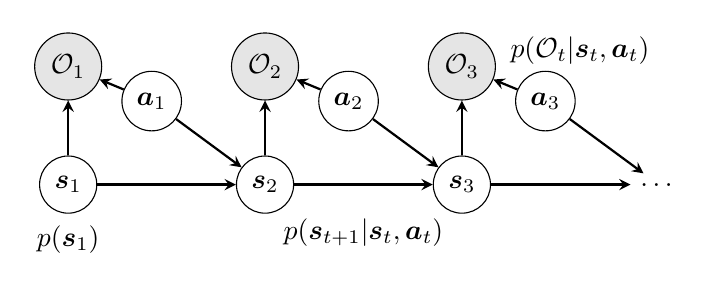
\begin{tikzpicture}[scale=1, transform shape, node distance=1.5cm]
		\node (s1) [mcs] {$\bm{s}_{1} $};
		\node (descs1) [below of=s1, yshift=0.8cm] { $ p (\bm{s}_{1})  $ };
		\node (o1) [mcsb, above of=s1] {$\mathcal{O}_{ 1 }$};
		\draw [arrow] (s1) -- (o1);
		\node (a1) [mcs, above right of=s1] { $ \bm{a}_{1}  $};
		\draw [arrow] (a1) -- (o1);
		\node (s2) [mcs, right of=s1, xshift=1cm] { $ \bm{s}_{2}  $};
		\node (o2) [mcsb, above of=s2] {$\mathcal{O}_{ 2 }$};
		\draw [arrow] (s1) -- (s2);
		\draw [arrow] (a1) -- (s2);
		\draw [arrow] (s2) -- (o2);
		\node (a2) [mcs, above right of=s2] { $ \bm{a}_{2}  $};
		\draw [arrow] (a2) -- (o2);
		\node (s3) [mcs, right of=s2, xshift=1cm] { $ \bm{s}_{3}  $};
		\draw [arrow] (a2) -- (s3);
		\draw [arrow] (s2) -- node [midway, below, yshift=-0.3cm] {$p (\bm{s}_{t+1}|\bm{s}_{t}, \bm{a}_{t})  $ }  (s3);
		\node (o3) [mcsb, above of=s3] {$\mathcal{O}_{ 3 }$};
		\node (desco3) [right of=o3, yshift=0.2cm] { $ p (\mathcal{O}_{ t }|\bm{s}_{t}, \bm{a}_{t})  $ };
		\node (a3) [mcs, above right of=s3] { $ \bm{a}_{3}  $};
		\draw [arrow] (s3) -- (o3);
		\draw [arrow] (a3) -- (o3);
		\node (s4) [right of=s3, xshift=1cm] {$\dots$};
		\draw [arrow] (s3) -- (s4);
		\draw [arrow] (a3) -- (s4);
\end{tikzpicture}
\end{center}
\end{figure}

and now the graph of our approximate version $ q (\bm{s}_{1:T}, \bm{a}_{1:T})  $ looks like:

\begin{figure}[htpb]
		\caption{$ q (\bm{s}_{1:T}, \bm{a}_{1:T})  $}
\begin{center}
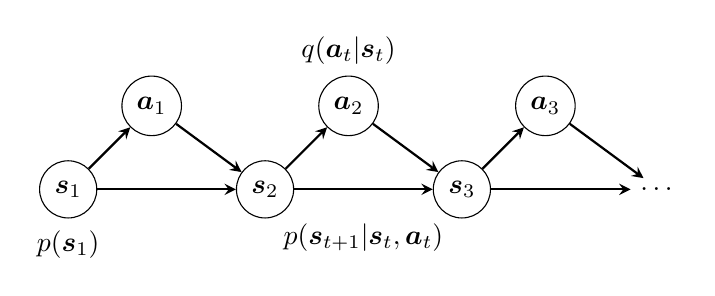
\begin{tikzpicture}[scale=1, transform shape, node distance=1.5cm]
		\node (s1) [mcs] {$\bm{s}_{1} $};
		\node (descs1) [below of=s1, yshift=0.8cm] { $ p (\bm{s}_{1})  $ };
		\node (a1) [mcs, above right of=s1] { $ \bm{a}_{1}  $};
		\node (s2) [mcs, right of=s1, xshift=1cm] { $ \bm{s}_{2}  $};
		\draw [arrow] (s1) -- (s2);
		\draw [arrow] (s1) -- (a1);
		\draw [arrow] (a1) -- (s2);
		\node (a2) [mcs, above right of=s2] { $ \bm{a}_{2}  $};
		\draw [arrow] (s2) -- (a2);
		\node (desca2) [above of=a2, yshift=-0.8cm] { $ q(\bm{a}_{t}| \bm{s}_{t} )  $};
		\node (s3) [mcs, right of=s2, xshift=1cm] { $ \bm{s}_{3}  $};
		\draw [arrow] (a2) -- (s3);
		\draw [arrow] (s2) -- node [midway, below, yshift=-0.3cm] {$p (\bm{s}_{t+1}|\bm{s}_{t}, \bm{a}_{t})  $ }  (s3);
		\node (a3) [mcs, above right of=s3] { $ \bm{a}_{3}  $};
		\draw [arrow] (s3) -- (a3);
		\node (s4) [right of=s3, xshift=1cm] {$\dots$};
		\draw [arrow] (s3) -- (s4);
		\draw [arrow] (a3) -- (s4);
\end{tikzpicture}
\end{center}
\end{figure}
Let's tie this back variational inference.
Let $ \bm{x}_{} = \mathcal{O}_{ 1:T }  $ and $ \bm{z}_{} = (\bm{s}_{1:T}, \bm{a}_{1:T} )  $.
Now we want to write $ p (\bm{z}_{}|\bm{x}_{})  $ and $ q (\bm{z}_{})  $

\subsection{Variational lower bound}
\begin{align}
		\log p (\bm{x}_{}) &\geq E_{ \bm{z}_{} \sim q (\bm{x}_{}) } \left[  \log p (\bm{x}_{}, \bm{z}_{}) - 
\underbrace{\log q (\bm{z}_{})}_{ \text{entropy } \mathcal{H}(q) } \right] 
\end{align}
let (just substituting the new definitions)
\begin{equation}
q (\bm{s}_{1:T}, \bm{a}_{1:T} ) = p (\bm{s}_{1}) \prod_{t}^{} p (\bm{s}_{t+1}|\bm{s}_{t}, \bm{a}_{t}) q(\bm{a}_{t}| \bm{s}_{t} )
\end{equation}
and now we can write the log probability of evidence:
(align + plus split left the broken env, 
but at least youcan see the eqs, i can't be bothered atm)
\begin{align}
		\log p (\mathcal{O}_{ 1:T }) &\geq 
		E_{ (\bm{s}_{1:T}, \bm{a}_{1:T} ) \sim q }
		[ 
				\cancel{\log p (\bm{s}_{1})} + \cancel{ \sum_{t=1}^{T} \log p (\bm{s}_{t+1}|\bm{s}_{t}, \bm{a}_{t})} \nonumber \\
									 &+ 
		\sum_{t=1}^{T} \log p (\mathcal{O}_{ t }| \bm{s}_{t}, \bm{a}_{t}) - 
		\cancel{\log p (\bm{s}_{1})} \nonumber \\ &- 
\cancel{\sum_{t=1}^{T} \log p (\bm{s}_{t+1}|\bm{s}_{t}, \bm{a}_{t}) }
- \sum_{t=1}^{T} \log q (\bm{a}_{t}| \bm{s}_{t} )
] \nonumber \\
&= E_{  (\bm{s}_{1:T}, \bm{a}_{1:T} ) \sim q  } \left[ \sum_{t}^{} r(\bm{s}_{t}, \bm{a}_{t} ) - \log q(\bm{a}_{t}| \bm{s}_{t} ) \right] \\
&= \sum_{t}^{} E_{ (\bm{s}_{t}, \bm{a}_{t} ) \sim q } \left[ r(\bm{s}_{t}, \bm{a}_{t} ) + \mathcal{H} (q (\bm{a}_{t}| \bm{s}_{t} )) \right] 
\end{align}
and from this we can see that we got the RL objective plus the additional entropy terms
which model the slighly suboptimal behavior.

\subsection{Optimizing the variational lower bound}
Let's restate the relevant equations. Here's our q:
\begin{equation}
q (\bm{s}_{1:T}, \bm{a}_{1:T} ) = p (\bm{s}_{1}) \prod_{t}^{} p (\bm{s}_{t+1}|\bm{s}_{t}, \bm{a}_{t}) q (\bm{a}_{t}| \bm{s}_{t} )
\end{equation}
and
the bound:
\begin{equation}
		\log p (\mathcal{O}_{ 1:T }) \geq
		\sum_{t}^{} E_{ (\bm{s}_{t}, \bm{a}_{t} )\sim q} 
		\left[ r(\bm{s}_{t}, \bm{a}_{t} ) + \mathcal{H} (q(\bm{a}_{t}| \bm{s}_{t} )) \right] 
\end{equation}
We could employ the dynamic programming approach:
\begin{align}
		q(\bm{a}_{T}| \bm{s}_{T} ) 
		&= \argmax_{} E_{ \bm{s}_{T} \sim q (\bm{s}_{T}) } \left[ 
E_{ \bm{a}_{T}\sim q(\bm{a}_{T}| \bm{s}_{T} ) } \left[ r (\bm{s}_{T}, \bm{a}_{T} ) \right] 
+ \mathcal{H} (q(\bm{a}_{T}| \bm{s}_{T} ))
\right] \\
&= \argmax_{} E_{ \bm{s}_{T} \sim q (\bm{s}_{T}) } \left[ 
E_{ \bm{a}_{T}\sim q(\bm{a}_{T}| \bm{s}_{T} ) } \left[ r (\bm{s}_{T}, \bm{a}_{T} ) 
- \log (q(\bm{a}_{T}| \bm{s}_{T} ))
\right] \right] 
\end{align}
It can be shown that anytime you have an optimization objective of form
of the expected value under a distribution of some quantity - the log
probability of that distribution,
the solution is always the exponential of that quantity.
So we get that $ q(\bm{a}_{T}| \bm{s}_{T} )  $ is optimized when
\begin{equation}
		q(\bm{a}_{T}| \bm{s}_{T} ) \propto \exp (r(\bm{s}_{T}, \bm{a}_{T} ))
\end{equation}
and in particular we get
\begin{equation}
		q(\bm{a}_{T}| \bm{s}_{T} ) =
		\frac{\exp (r(\bm{s}_{T}, \bm{a}_{T} ))}{\int \exp (r(\bm{s}_{T}, \bm{a}_{} ))d\bm{a}_{}} = 
		\exp (Q(\bm{s}_{T}, \bm{a}_{T} ) - V (\bm{s}_{T}))
\end{equation}
\begin{equation}
		V (\bm{s}_{T}) = \log \int \exp (Q(\bm{s}_{T}, \bm{a}_{T} ))d \bm{a}_{T}
\end{equation}
If we substitu in the expression for $ Q  $ we get:
\begin{equation}
E_{ \bm{s}_{T}\sim q (\bm{s}_{T}) }
\left[ 
E_{ \bm{a}_{T} \sim q(\bm{a}_{T}| \bm{s}_{T} ) }
\left[ 
r(\bm{s}_{T}, \bm{a}_{T} ) - \log q(\bm{a}_{T}| \bm{s}_{T} )
\right] 
\right] 
=
E_{ \bm{s}_{T}\sim q (\bm{s}_{T}) } \left[ 
E_{ \bm{a}_{T} \sim q(\bm{a}_{T}| \bm{s}_{T} ) } \left[ V (\bm{s}_{T}) \right] 
\right] 
\end{equation}
and now we can proceed with the recursive case:
\begin{equation}
\begin{split}
q(\bm{a}_{t}| \bm{s}_{t} ) =
\argmax_{}
E_{ \bm{s}_{t}\sim q (\bm{s}_{t}) }
\left[ 
E_{ \bm{a}_{t} \sim q(\bm{a}_{t}| \bm{s}_{t} ) }
\left[ 
r(\bm{s}_{t}, \bm{a}_{t} ) - \log q(\bm{a}_{t}| \bm{s}_{t} ) 
+ E_{ \bm{s}_{t+1}\sim p (\bm{s}_{t+1}|\bm{s}_{t}, \bm{a}_{t}) }
\left[ V (\bm{s}_{t+1}) \right] 
\right] 
+ \mathcal{H} (q(\bm{a}_{t}| \bm{s}_{t} ))
\right] 
\end{split}
\end{equation}
we can use the regular (\textit{not} optimistic) Bellman backup
\begin{equation}
		Q_{ t }(\bm{s}_{t}, \bm{a}_{t} ) = r(\bm{s}_{t}, \bm{a}_{t} ) + E \left[ V_{ t+1 } (\bm{s}_{t+1}) \right] 
\end{equation}
and now continue:
\begin{align}
q(\bm{a}_{t}| \bm{s}_{t} ) &= \dots \\
&= \argmax_{} E_{ \bm{s}_{t} \sim q (\bm{s}_{t}) } \left[ 
E_{ \bm{a}_{t} \sim q(\bm{a}_{t}| \bm{s}_{t} ) } \left[ 
Q(\bm{s}_{t}, \bm{a}_{t} ) + \mathcal{H} (q(\bm{a}_{t}| \bm{s}_{t} ))
\right] 
\right] \\
&= \argmax_{} E_{ \bm{s}_{t} \sim q (\bm{s}_{t}) } \left[ 
E_{ \bm{a}_{t} \sim q(\bm{a}_{t}| \bm{s}_{t} ) } \left[ 
Q(\bm{s}_{t}, \bm{a}_{t} ) - \log (q(\bm{a}_{t}| \bm{s}_{t} ))
\right] 
\right] \\
& \text{optimized when } q(\bm{a}_{t}| \bm{s}_{t} ) \propto \exp (Q(\bm{s}_{t}, \bm{a}_{t} ))\\
& \text{the normalizer is } V_{ t } (\bm{s}_{t}) = \log \int \exp (Q_{ t }(\bm{s}_{t}, \bm{a}_{t} )) d\bm{a}_{t}\\
& \text{and we get } \exp (Q (\bm{s}_{t}, \bm{a}_{t} ) - V (\bm{s}_{t}))
\end{align}
we can formalize the recursive solution as a backward pass.
If you'll want more on this check out Levine 2018
reinforcement learning and control as probabilistic inferece: tutorial and review (downloaded and ready in master's folder).
You can also add discount or explicit temperature to this.

\section{Algorithms for RL as inference}
\subsection{Q-learning with soft optimality}
The stardard Q-learning looks like this:
\begin{align}
\text{standard Q-learning: }& \phi \leftarrow \phi \alpha \nabla_{ \phi } Q_{ \phi } (\bm{s}_{}, \bm{a}_{} )
\left( r (\bm{s}_{}, \bm{a}_{} ) + \gamma V (\bm{s}_{}') - Q_{ \phi } (\bm{s}_{}, \bm{a}_{} ) \right)  \\
\text{target value: } & V (\bm{s}_{}') = \max_{\bm{a}_{}'} Q_{ \phi } (\bm{s}_{}', \bm{a}_{} ')
\end{align}
We could instead use soft optimality and have:
\begin{align}
\text{soft Q-learning: }& \phi \leftarrow \phi \alpha \nabla_{ \phi } Q_{ \phi } (\bm{s}_{}, \bm{a}_{} )
\left( r (\bm{s}_{}, \bm{a}_{} ) + \gamma V (\bm{s}_{}') - Q_{ \phi } (\bm{s}_{}, \bm{a}_{} ) \right)  \\
\text{target value: }& V (\bm{s}_{}') =\text{soft } \max_{\bm{a}_{}'} Q_{ \phi } (\bm{s}_{}', \bm{a}_{} ') = \log \int \exp (Q_{ \phi }(\bm{s}_{}', \bm{a}_{}' )) d\bm{a}_{}'\\
\text{policy: } & \exp (Q_{ \phi }(\bm{s}_{}, \bm{a}_{} ) - V (\bm{s}_{})) = \exp (A(\bm{s}_{}, \bm{a}_{} ))
\end{align}
and the resulting Q-learning with soft optimality algorithm looks like:
\begin{enumerate}
		\item take some action $\bm{a}_i$,  observe $\left( \bm{s}_i, \bm{a}_i, \bm{s}_i', r_i \right)$ and add it to $\mathcal{R}$
		\item sample a mini-batch  $\left( \bm{s}_j, \bm{a}_j, \bm{s}_j', r_j \right)$  from $\mathcal{R}$ uniformly
		\item compute $y_j = r_j + \gamma \text{soft} \max_{\bm{a}_j'} Q_{\phi'} (\bm{s}_{j}', \bm{a}_{j}')$ using \textit{target} network $Q_{\phi'}$
		\item $  \phi \leftarrow \phi  - \alpha \sum_{j}^{}  \frac{d Q_\phi}{d\phi} (\bm{s}_{j}, \bm{a}_{j}) \left( Q_\phi(\bm{s}_{i}, \bm{a}_{i}) - 
				y_j 	\right) $ 
		\item update $\phi'$: copy $\phi$ every $N$ steps, or Polyak average $ \phi' \leftarrow \tau \phi' + (1 - \tau) \phi  $
\end{enumerate}
So pretty much the same as standard Q-learning, except for the softmax.

\subsection{Policy gradient with soft optimality}
\begin{equation}
		\pi (\bm{a}_{}| \bm{s}_{} ) = \exp \left( Q_{ \phi } (\bm{s}_{}, \bm{a}_{} ) - V (\bm{s}_{}) \right) 
\end{equation}
optimizes
\begin{equation}
\sum_{t}^{} E_{ \pi (\bm{s}_{t}, \bm{a}_{t} ) } \left[ r(\bm{s}_{t}, \bm{a}_{t} ) \right] + 
E_{ \pi (\bm{s}_{t}) } \left[  \mathcal{H} (\pi(\bm{a}_{t}| \bm{s}_{t} ))
\right] 
\end{equation}
where $ \mathcal{H} (\pi(\bm{a}_{t}| \bm{s}_{t} ))  $ is the policy entropy and that's the only new thing.
The intuition is that the policy $ \pi(\bm{a}_{}| \bm{s}_{} )  \propto \exp (Q_{ \phi }(\bm{s}_{}, \bm{a}_{} ))$ 
when $ \pi   $ minimizes $ D_{ KL } (\pi (\bm{a}_{}| \bm{s}_{} ) || \frac{1}{Z} \exp (Q(\bm{s}_{}, \bm{a}_{} ))  ) $  
This is often referred to as ``entropy regularized'' policy gradient and it combats
premature entropy collapse (when policy becomes deterministic too early).

\subsection{Policy gradient vs Q-learning}
\begin{equation}
		J (\theta) = \sum_{t}^{} E_{ \pi (\bm{s}_{t}, \bm{a}_{t} ) } \left[ r (\bm{s}_{t}, \bm{a}_{t} ) \right] +
		\underbrace{E_{ \pi (\bm{s}_{t}) } \left[ \mathcal{H} (\pi (\bm{a}_{t}| \bm{s}_{t} )) \right] }_{ E_{ \pi (\bm{a}_{t}| \bm{s}_{t} ) } \left[ - \log \pi (\bm{a}_{t}| \bm{s}_{t} ) \right]  }
		= \sum_{t}^{} E_{ \pi (\bm{s}_{t}, \bm{a}_{t} ) } \left[ r (\bm{s}_{t}, \bm{a}_{t} ) - \log \pi(\bm{a}_{t}| \bm{s}_{t} ) \right] 
\end{equation}
and the gradient w.r.t $ \theta  $ is:
\begin{flalign}
&		\nabla_{ \theta } \left[ \sum_{t}^{} E_{ \pi (\bm{s}_{t}, \bm{a}_{t} ) } \left[ r(\bm{s}_{t}, \bm{a}_{t} ) - \log \pi (\bm{a}_{t}| \bm{s}_{t} ) \right]  \right] & \nonumber \\
&\approx \frac{1}{N} \sum_{i}^{} \sum_{t}^{} \nabla_{ \theta } \log \pi (\bm{a}_{t}| \bm{s}_{t} ) 
\left(
\underbrace{ r (\bm{s}_{t}, \bm{a}_{t} ) + \left( \sum_{t'=t+1}^{T} r (\bm{s}_{t'}, \bm{a}_{t'} ) - \log \pi (\bm{a}_{t'}| \bm{s}_{t'} ) \right) }_{ \approx Q (\bm{s}_{t+1}, \bm{a}_{t+1} ) }
- \log \pi (\bm{a}_{t}| \bm{s}_{t} ) -1 \right) &
\end{flalign}
But since the $ -1  $ doesn't make a difference when taking the gradient,
you can just remove it and so it turns out that if you want to entropy regularize
the policy, you just need to $ - \log \pi (\bm{a}_{t}| \bm{s}_{t} )  $ to the expression you're taking a gradient of.
If we use $ \log \pi (\bm{a}_{t}| \bm{s}_{t} ) = Q (\bm{s}_{t}, \bm{a}_{t} ) - V (\bm{s}_{t}) $
we can futher reduce the expression into
\begin{equation}
\approx \frac{1}{N} \sum_{i}^{} \sum_{t}^{} \left(   \nabla_{ \theta } Q (\bm{a}_{t}| \bm{s}_{t} ) - \nabla_{ \theta } V (\bm{s}_{t})  \right) 
\left( r (\bm{s}_{t}, \bm{a}_{t} ) + Q (\bm{s}_{t+1}, \bm{a}_{t+1} ) - Q (\bm{s}_{t}, \bm{a}_{t} ) + \cancel{V (\bm{s}_{t})} \right) 
\end{equation}
where we again remove a baseline term.
Q-learning grad descent under softmax is:
\begin{equation}
- \frac{1}{N} \sum_{i}^{} \sum_{t}^{}\nabla_{ \theta } Q (\bm{a}_{t}| \bm{s}_{t} ) \left( 
r(\bm{s}_{t}, \bm{a}_{t} ) + 
\underbrace{\text{soft} \max_{\bm{a}_{t+1}} Q (\bm{s}_{t+1}, \bm{a}_{t+1} ) }_{ \text{off-policy correction} }
- Q (\bm{s}_{t}, \bm{a}_{t} )
\right)  
\end{equation}
so these 2 are quite similar under the soft optimality framework.
\subsection{Benefits of soft optimality}
\begin{itemize}
		\item imrove exploration and prevent entropy collapse
		\item easier to specialize (fineture) policies for more specific tasks
		\item principled approach to break ties
		\item better robustness (due to wider coverage of states)
		\item can reduce to hard optimality as reward magnitude increases, or if you put in temperature and drive it to 0
		\item good model for modeling human behavior
\end{itemize}

\subsection{Example methods}
Some papers using these methods, skippable.
Includes SAC.

\chapter{Inverse reinforcement learning}
So far we always assumed that a reward function was provided (and it was in fact hand-engineered).
But what if we could \textit{learn}  the reward function from observing an expert, and then use reinforcement learning?
We'll utilize the approximate optimality model from last time, but now we'll learn the reward.
We defined optimality in the deterministic case:
\begin{align}
		\bm{a}_{1}, \dots, \bm{a}_{T} &= \argmax_{\bm{a}_{1}, \dots, \bm{a}_{T}} \sum_{t=1}^{T} r(\bm{s}_{t}, \bm{a}_{t} ) \\
		\bm{s}_{t+1} &= f(\bm{s}_{t}, \bm{a}_{t} )
\end{align}
and in the stochastic case:
\begin{align}
		\pi &= \argmax_{\pi} E_{ \bm{s}_{t+1} \sim p (\bm{s}_{t+1}| \bm{s}_{t}, \bm{a}_{t} ), \bm{a}_{t} \sim \pi (\bm{a}_{t}| \bm{s}_{t} ) } \left[ r (\bm{s}_{t}, \bm{a}_{t} ) \right] 	\\
		\bm{a}_{t} \sim \pi (\bm{a}_{t}| \bm{s}_{t} )
\end{align}

\subsection{Why should we worry about learning rewards?}
\subsubsection{Imitation learning perspective}
Why not do imitation learning? Well, humans don't do it this way.
Humans try to understand what others do --- we copy the \textit{intent} of the expert.
This might result in very different actions.

\subsubsection{The RL perspective}
What is the reward for a car going down the highway? It's probably much easier
to have a professional driver demonstrate good driver than to hand-engineer reward function.

\subsubsection{Inverse RL}
By itself, this is an \textbf{underspecified} problem --- many reward function can explain the \textbf{same} behavior.
Take a gridworld example. A sample trajectory can does not tell you what the reward was. Was it going to that square, 
all squares in some area, etc.

\begin{table}[htpb]
		\centering
		\begin{tabular}{c | c}
				\textbf{``forward RL''} & \textbf{inverse RL} \\
				\hline
				given: &  given: \\
				states $ \bm{s}_{} \in \mathcal{S}  $, actions $ \bm{a}_{} \in \mathcal{A}  $ &
				states $ \bm{s}_{} \in \mathcal{S}  $, actions $ \bm{a}_{} \in \mathcal{A}  $ \\
				(sometimes) transitions $ p (\bm{s}_{}'|\bm{s}_{}, \bm{a}_{} )  $ &
				(sometimes) transitions $ p (\bm{s}_{}'|\bm{s}_{}, \bm{a}_{} )  $\\
				reward function $ r \bm{s}_{}, \bm{a}_{}   $ &
				samples $ \left\{ \tau_{ i } \right\}   $ sampled from $ \pi^{ \star } (\tau)  $ \\
				learn $ \pi^{ \star } (\bm{a}_{}| \bm{s}_{} )  $&
				learn $ \pi_{ \psi } (\bm{s}_{}, \bm{a}_{} )  $ ($\psi$ are the reward params)\\
				\hline
		\end{tabular}
\end{table}

\subsection{Feature matching IRL}
The pre-neural net stuff.
Linear reward functions were used:
\begin{equation}
		r_{ \psi } (\bm{s}_{}, \bm{a}_{} ) =
		\sum_{i}^{} \psi_{ i } f_{ i } (\bm{s}_{}, \bm{a}_{} ) = \psi^{ T } \bm{f}_{} (\bm{s}_{}, \bm{a}_{} )
\end{equation}
if features $ \bm{f}_{}  $ are important, what if we match their expectations?
So let $ \pi^{ r_{ \psi } }  $ be optimal policy for $ r_{ \psi }  $.
Pick $ \psi  $ s.t. $   
E_{ \pi^{ r_{ \psi } } } \left[ \bm{f}_{} (\bm{s}_{}, \bm{a}_{} )  \right] 
= E_{ \pi^{ \star } } \left[ \bm{f}_{} (\bm{s}_{}, \bm{a}_{} ) \right] $,
where $ E_{ \pi^{ r_{ \psi } } } \left[ \bm{f}_{} (\bm{s}_{}, \bm{a}_{} )  \right]  $ is the state-action marginal under $ \pi^{ r_{ \psi } }  $ 
and  $ E_{ \pi^{ \star } } \left[ \bm{f}_{} (\bm{s}_{}, \bm{a}_{} ) \right]   $ is the unknown optimal policy approximated using expert samples.
Well, this is still ambiguous because multiple different $ \psi_{ i }  $
could result in the same policy.
One thing people thought of is
\begin{equation}
		\max_{\psi, m} m \text{ such that } \psi^{ T } E_{ \pi^{ \star } } \left[ \bm{f}_{}(\bm{s}_{}, \bm{a}_{} ) \right] 
		\geq \max_{\pi \in \Pi} \psi^{ T } E_{ \pi } \left[ \bm{f}_{}(\bm{s}_{}, \bm{a}_{} ) \right]  +m
\end{equation}
this is a heuristic, but it's reasonable. Basically it says to pick the reward for which the expert is the best.
But we need to somehow ``weight'' $ \pi^{ \star }  $ and $ \pi  $ by similarity.
This stuff is from support vector machines (SVMs).
I'll casually skip how to do this with SVMs.
The problems with this are the following:
\begin{itemize}
		\item maximizing the margin is a bit arbitrary
		\item it does not provide a clear model of expert suboptimality 
		\item it results in a messy constrained optimization problem --- not great for deep learning
\end{itemize}

In our graphical model with optimality probabilities $ p (\mathcal{O}| \bm{s}_{t}, \bm{a}_{t} ) = \exp (r (\bm{s}_{t}, \bm{a}_{t} ))  $,
we calculated the probability of a trajectory, given that the actor acts optimally and that gave us
that the optimal trajectory was the most likely and that the suboptimal trajectories were less likely:
\begin{align}
		p (\tau|\mathcal{O}_{ 1:T }) &= \frac{p (\tau, \mathcal{O}_{ 1:T })}{p (\mathcal{O}_{ 1:T })}  \\
&\propto p (\tau) \prod_{t}^{} \exp (r (\bm{s}_{t}, \bm{a}_{t} )) = p (\tau) \exp \left( \sum_{t}^{} r (\bm{s}_{t}, \bm{a}_{t} ) \right)  
\end{align}

But now we'll use this model to learn reward functions.

\subsection{Learning the optimality variable}

\begin{figure}[htpb]
		\caption{$ p (\bm{s}_{1:T}, \bm{a}_{1:T}|\mathcal{O}_{ 1:T })  $}
\begin{center}
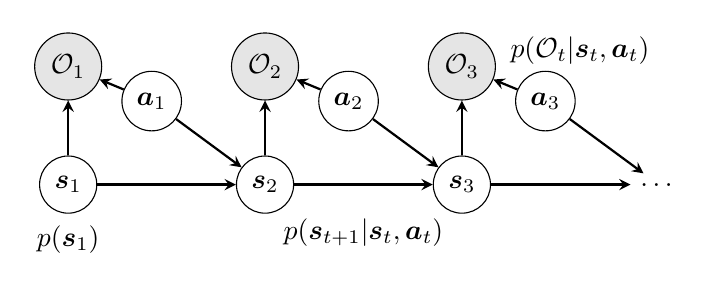
\begin{tikzpicture}[scale=1, transform shape, node distance=1.5cm]
		\node (s1) [mcs] {$\bm{s}_{1} $};
		\node (descs1) [below of=s1, yshift=0.8cm] { $ p (\bm{s}_{1})  $ };
		\node (o1) [mcsb, above of=s1] {$\mathcal{O}_{ 1 }$};
		\draw [arrow] (s1) -- (o1);
		\node (a1) [mcs, above right of=s1] { $ \bm{a}_{1}  $};
		\draw [arrow] (a1) -- (o1);
		\node (s2) [mcs, right of=s1, xshift=1cm] { $ \bm{s}_{2}  $};
		\node (o2) [mcsb, above of=s2] {$\mathcal{O}_{ 2 }$};
		\draw [arrow] (s1) -- (s2);
		\draw [arrow] (a1) -- (s2);
		\draw [arrow] (s2) -- (o2);
		\node (a2) [mcs, above right of=s2] { $ \bm{a}_{2}  $};
		\draw [arrow] (a2) -- (o2);
		\node (s3) [mcs, right of=s2, xshift=1cm] { $ \bm{s}_{3}  $};
		\draw [arrow] (a2) -- (s3);
		\draw [arrow] (s2) -- node [midway, below, yshift=-0.3cm] {$p (\bm{s}_{t+1}|\bm{s}_{t}, \bm{a}_{t})  $ }  (s3);
		\node (o3) [mcsb, above of=s3] {$\mathcal{O}_{ 3 }$};
		\node (desco3) [right of=o3, yshift=0.2cm] { $ p (\mathcal{O}_{ t }|\bm{s}_{t}, \bm{a}_{t})  $ };
		\node (a3) [mcs, above right of=s3] { $ \bm{a}_{3}  $};
		\draw [arrow] (s3) -- (o3);
		\draw [arrow] (a3) -- (o3);
		\node (s4) [right of=s3, xshift=1cm] {$\dots$};
		\draw [arrow] (s3) -- (s4);
		\draw [arrow] (a3) -- (s4);
\end{tikzpicture}
\end{center}
\end{figure}

\begin{equation}
		p (\mathcal{O}_{ t }| \bm{s}_{t}, \bm{a}_{t} , \psi) = \exp (r_{ \psi }(\bm{s}_{t}, \bm{a}_{t} ))
\end{equation}
From before we have
\begin{equation}
		p (\tau|\mathcal{O}_{ 1:T },\psi )
		\propto 
		\underbrace{\cancel{p (\tau)} }_{ \text{can ignore 'cos independent of } \psi}
		\exp \left( \sum_{t}^{} r_{ \psi } (\bm{s}_{t}, \bm{a}_{t} ) \right) 
\end{equation}
In the inverse RL setting we're given samples $ \left\{ \tau_{ i } \right\}   $ from $ \pi^{ \star } (\tau)  $
and we can do maximum likelihood learning on that:
\begin{equation}
		\max_{\psi} \frac{1}{N}  \sum_{i=1}^{N} \log p (\tau_{ i }|\mathcal{O}_{ 1:T }, \psi)
		= 
		\max_{\psi} \frac{1}{N}  \sum_{i=1}^{N} r_{ \psi } (\tau_{ i } ) -\log Z
\end{equation}
where we plugged in our $ p (\tau|\mathcal{O}_{ 1:T },\psi)  $ expression in.
The log normalized $ \log Z  $, also know as the partition function
is making RL difficult.

\subsubsection{The IRL partition function}
We're looking at:
\begin{equation}
		\max_{\psi} \frac{1}{N} \sum_{i=1}^{N} r_{ \psi } (\tau_{ i }) -\log Z
\end{equation}
where $ Z  $ is
\begin{equation}
		Z = \int p (\tau) \exp (r_{ \psi } (\tau)) d\tau
\end{equation}
The $ Z  $ will prove to be intractable to compute.
We could try to plug this in and take the derivative and we'd get the following
\begin{equation}
\nabla_{ \psi } \mathcal{L} = 
\frac{1}{N}  \sum_{i=1}^{N} \nabla_{ \psi } r_{ \psi } (\tau_{ i })
- 
\underbrace{\frac{1}{Z} \int p (\tau) \exp (r_{ \psi (\tau) }) }_{ p (\tau| \mathcal{O}_{ 1:T }, \psi) }
\nabla_{ \psi } r_{ \psi } (\tau) d\tau
\end{equation}
and so we can equivalently write the gradient in terms of expectations:
\begin{equation}
\nabla_{ \psi } \mathcal{L} = 
\underbrace{E_{ \tau \sim \pi^{ \star } (\tau) } \left[ \nabla_{ \psi } r_{ \psi } (\tau_{ i })\right] }_{ \text{estimate with expert samples} }
- 
\underbrace{E_{ \tau \sim p (\tau|\mathcal{O}_{ 1:T }, \psi) } \left[ \nabla_{ \psi } r_{ \psi } (\tau) \right] }_{ \text{soft optimal policy under current reward} }
\end{equation}
and this has the following nice interpretation:
the gradient of maximum likelihood of $ \psi  $
is the difference between the expected value of the gradient obtained through optimal policy $ \pi^{ \star }  $
and the expected value of the gradient under the current reward (which isdependent on $ \psi  $).
And it since these are expectations, they can be sampled and we can create an algorithm out of this.
Let's talk about how we can perform the estimation of the policy under current reward.

\subsubsection{Estimating the expectation}
Let's make the second expectation a bit more explicit:
\begin{align}
E_{ \tau \sim p (\tau|\mathcal{O}_{ 1:T }, \psi) } \left[ \nabla_{ \psi } r_{ \psi } (\tau) \right] &=
E_{ \tau \sim p (\tau|\mathcal{O}_{ 1:T }, \psi) }
\left[ \nabla_{ \psi } \sum_{t=1}^{T} r_{ \psi } (\bm{s}_{t}, \bm{a}_{t} ) \right] \\
&= \sum_{t=1}^{T} 
E\underbrace{_{ (\bm{s}_{t}, \bm{a}_{t} ) \sim p (\bm{s}_{t}, \bm{a}_{t} | \mathcal{O}_{ 1:T }, \psi) }}_{ 
p (\bm{a}_{t}|\bm{s}_{t}, \mathcal{O}_{ 1:T },\psi) p (\bm{s}_{t}|\mathcal{O}_{ 1:T } , \psi)}
\left[ \nabla_{ \psi }r_{ \psi } (\bm{s}_{t}, \bm{a}_{t} ) \right] 
\end{align}
and we've seen that 
\begin{equation}
	p (\bm{a}_{t}|\bm{s}_{t}, \mathcal{O}_{ 1:T },\psi)
	= \frac{\beta (\bm{s}_{t}, \bm{a}_{t} )}{\beta (\bm{s}_{t})} 
\end{equation}
and 
\begin{equation}
		p (\bm{s}_{t}|\mathcal{O}_{ 1:T } , \psi) \propto \alpha (\bm{s}_{t}) \beta (\bm{s}_{t}) 
\end{equation}
and we also know that
\begin{equation}
		 (\bm{s}_{t}, \bm{a}_{t} ) \sim p (\bm{s}_{t}, \bm{a}_{t} | \mathcal{O}_{ 1:T }, \psi) 
		 \propto \beta (\bm{s}_{t}, \bm{a}_{t} ) \alpha (\bm{s}_{t})
\end{equation}
This last thing has to be normalized over states and actions, but not over trajectories,
so it's more tractable.
Let's introduce simplifying notation:
\begin{equation}
	\mu_{ t } (\bm{s}_{t}, \bm{a}_{t} )\propto \beta (\bm{s}_{t}, \bm{a}_{t} ) \alpha (\bm{s}_{t})	
\end{equation}
Now we can get:
\begin{align}
E_{ \tau \sim p (\tau|\mathcal{O}_{ 1:T }, \psi) } \left[ \nabla_{ \psi } r_{ \psi } (\tau) \right] &=
\sum_{t=1}^{T} \int \int \mu_{ t } (\bm{s}_{t}, \bm{a}_{t} ) \nabla_{ \psi }r_{ \psi } (\bm{s}_{t}, \bm{a}_{t} ) d\bm{s}_{t}d\bm{a}_{t} \\
&= \sum_{t=1}^{T} \vec{\mu}_{ t }^{ T }\nabla_{ \psi }\vec{r}_{ \psi }
\end{align}
While this won't work for large state-action spaces, it's feasible for small discrete ones.
The $ \vec{\mu}_{ t }$ is the state-action visitation probability for each $ (\bm{s}_{t}, \bm{a}_{t} )  $.

\subsubsection{The MaxEnt IRL algorithm}
\begin{enumerate}
		\item given $ \psi  $, compute backward message $ \beta (\bm{s}_{t}, \bm{a}_{t} )  $
		\item given $ \psi  $, compute forward message $ \alpha (\bm{s}_{t})  $
		\item compute $ \mu_{ t }(\bm{s}_{t}, \bm{a}_{t} ) \propto \beta (\bm{s}_{t}, \bm{a}_{t} ) \alpha (\bm{s}_{t})$
		\item evaluate $ \nabla_{ \psi } \mathcal{L} = \frac{1}{N} \sum_{i=1}^{N} \sum_{t=1}^{T} \nabla_{ \psi }r_{ \psi } (\bm{s}_{i,t}, \bm{a}_{i,t} )
				- \sum_{t=1}^{T} \int \int \mu_{ t }(\bm{s}_{t}, \bm{a}_{t} )\nabla_{ \psi }r_{ \psi }(\bm{s}_{t}, \bm{a}_{t} )d\bm{s}_{t}d\bm{a}_{t}$
		\item $ \psi \leftarrow \psi + \eta \nabla_{ \psi } \mathcal{L}  $ and repeat until convergence
\end{enumerate}

This is called MaxEnt because in the case where
$ r_{ \psi }(\bm{s}_{t}, \bm{a}_{t} ) = \psi^{ T } \bm{f}_{}(\bm{s}_{t}, \bm{a}_{t} )  $,
we can show that it optimizes
\begin{equation}
	\max_{\psi} \mathcal{H} (\pi^{ r_{ \psi } }) \text{ such that } E_{ \pi^{ r_{ \psi } } } \left[ \bm{f}_{} \right] = E_{ \pi^{ \star } } \left[ \bm{f}_{} \right] 	
\end{equation}
so it's a kind of statistic reification of the Occam's razor.

\section{Approximations to higher dimensions}





























































\end{document}
